%This is the third chapter of the dissertation

%The following command starts your chapter. If you want different titles used in your ToC and at the top of the page throughout the chapter, you can specify those values here. Since Columbia doesn't want extra information in the headers and footers, the "Top of Page Title" value won't actually appear.

\pagestyle{cu}
\graphicspath{{./Chapter3/Figures/}}
\chapter[The XENON1T Dark Matter Search][The XENON1T Dark Matter Search]{The XENON1T Dark Matter Search}

% https://arxiv.org/pdf/1801.07231.pdf for electron emission from wires


XENON1T is the third generation experiment of the XENON collaboration.  With a fiducial mass of more than 1000 kg it is the first
liquid xenon dark matter (DM) detector to reach the ton-scale era of DM detection.  Its large target mass and low radioactive background
make it the most sensitive detector to spin-independent WIMPs with $m_{\chi} > 6\ \mathrm{GeV / c^2}$.

This chapter presents the run-combined analysis of Science Run 0 (SR0) and Science Run 1 (SR1) - the first two XENON1T dark matter
runs.  It begins with a description of the XENON1T experiment (\secref{sec:xenon1t_detector}), followed by discussions on detector
characterization (\secref{sec:det_char}) and backgrounds
(\secref{sec:backgrounds}).  The electronic and nuclear recoil band fittings are
then detailed (\secref{sec:er_nr_calibrations}) and finally dark matter search results (\secref{sec:dark_matter_results}) are
presented.  The original SR0-only analysis (\citeref{Aprile2017f}) is referred to as ``First Results'' and is cited for comparison.

\section{The XENON1T Detector}
\label{sec:xenon1t_detector}




\subsection{PMTs}
\label{subsec:xenon1t_pmts}
A total of 248 Hamamatsu R11410-21 PMTs are installed in XENON1T.  The 127 PMTs in the top array are positioned radially to
optimize the resolution of position reconstruction in $r$ (\secref{subsec:det_char_position_reconstruction}).  The 121 PMTs in the bottom
array
are packed as densely as possible to maximize light collection.  The most important characteristic of a PMT is its quantum efficiency
(QE), or the ratio of photoelectrons (electrons produced in the photocathode) divided by number of incident photons.  The R11410 window is
76.2 mm in diameter and the photocathode yields an average quantum efficiency for 178 nm of 34.5\% with 2.8\%
standard deviation (\citeref{Aprile2017b, Barrow2017}).

PMTs with the highest QEs are placed in the bottom array while those with the lowest are stationed along the circumference of the
top.  The difference in arrangement is strategic.  Due to liquid xenon's relatively large dielectric constant (1.95) photons
originating inside the liquid are likely to
reflect off the surface and be redirected towards the bottom of the TPC.  For low-energy events - the relevant range for WIMP DM
searches - nuclear recoils may only emit a small number ($\lesssim 100$) of photons, many of which never reach the PMTs.  Positioning
those with the highest quantum efficiency in the region most likely to see scintillation from an S1 captures more events and improves our
sensitivity.  S2s produce enough scintillation to be observed by both arrays.  Therefore the QE of the top PMTs is comparatively
unimportant, and could even be advantageous for large S2s that saturate the phototubes, though these events are outside the region of
interest for spin-independent WIMP dark matter.  The layout of the PMTs with their respective QE is shown
in \figref{fig:xenon1t_pmt_qe}.  The assembled PMT arrays are shown in \figref{fig:xenon1t_pmt_array}.

\begin{figure}
\centering
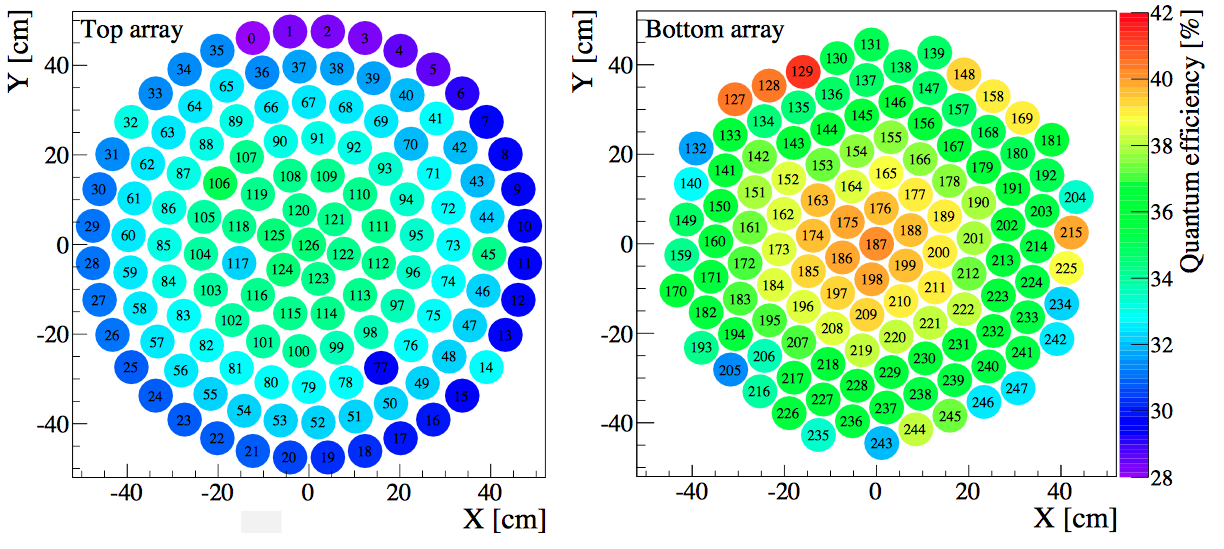
\includegraphics[width=\textwidth]{PMTQuantumEfficiency}
\caption{Quantum efficiency of top (left) and bottom (right) PMT arrays.  PMTs with the highest QE are placed in the center of the bottom
array to maximize light collection while those with the lowest are placed in the outermost region of the top.  Image credit:
\citeref{Aprile2017b}.}
\label{fig:xenon1t_pmt_qe}
\end{figure}

A photoelectron (PE) is a photon ejected by an incident photon on the photocathode.  It is guided by a focusing electrode disk to the
first of $N$ dynodes.  A voltage is applied to the photocathode and dynodes,
with each successive one (starting from the photocathode) lower than the previous.  Upon hitting the first dynode the photoelectron will
free some electrons in the first stage of an electron avalanche.  The electron avalanche will pass from dynode to dynode, rapidly
growing with each until it reaches the anode and is directed to the data acquisition.

\begin{figure}
    \centering
    \begin{subfigure}[t]{0.5\textwidth}
        \centering
        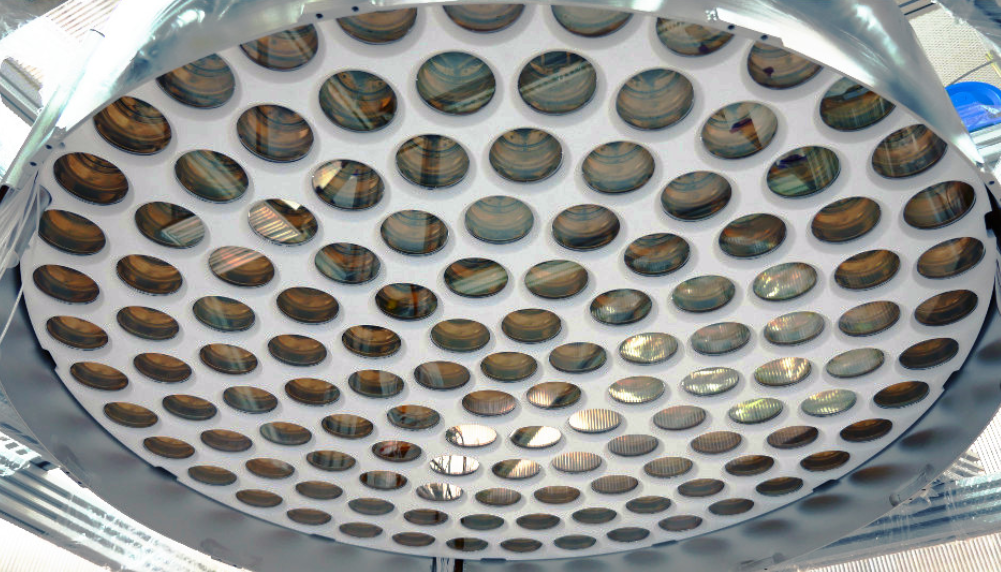
\includegraphics[height=4cm]{PMTTopArray}
    \end{subfigure}%
    \begin{subfigure}[t]{0.5\textwidth}
        \centering
        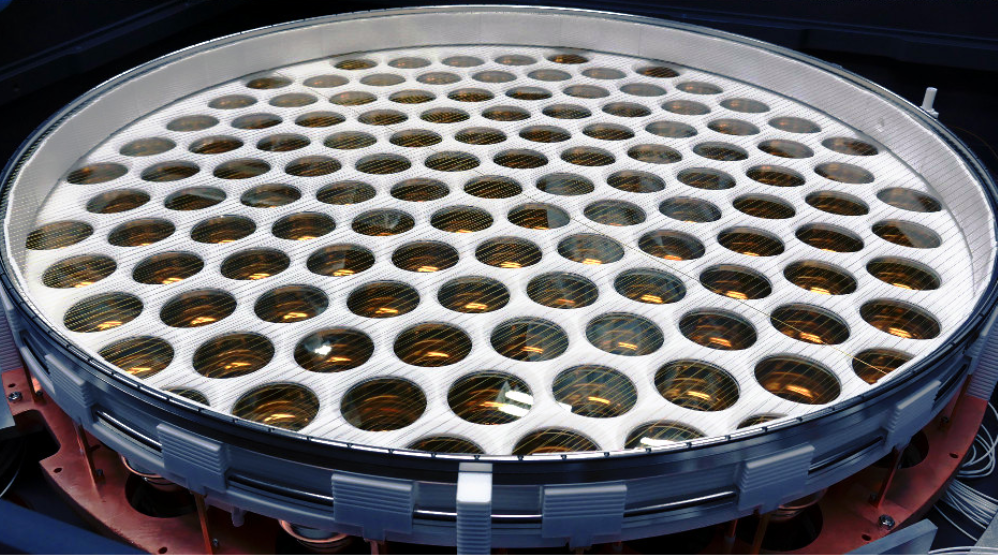
\includegraphics[height=4cm]{PMTBottomArray}
    \end{subfigure}
    \caption{Top (left) and bottom (right) PMT arrays.  Top PMTs are installed inside the diving bell above the anode and screening
    mesh in a radial distribution
    to minimize uncertainty in radial position reconstruction.  Bottom PMTs are packed tightly below the anode and a second screening mesh
    to optimize light collection.  The screening meshes reduce interference between the anode (cathode) and top (bottom) PMT electric
    fields.  Image credit: \citeref{Aprile2017b}.}
	\label{fig:xenon1t_pmt_array}
\end{figure}

\begin{figure}
\centering
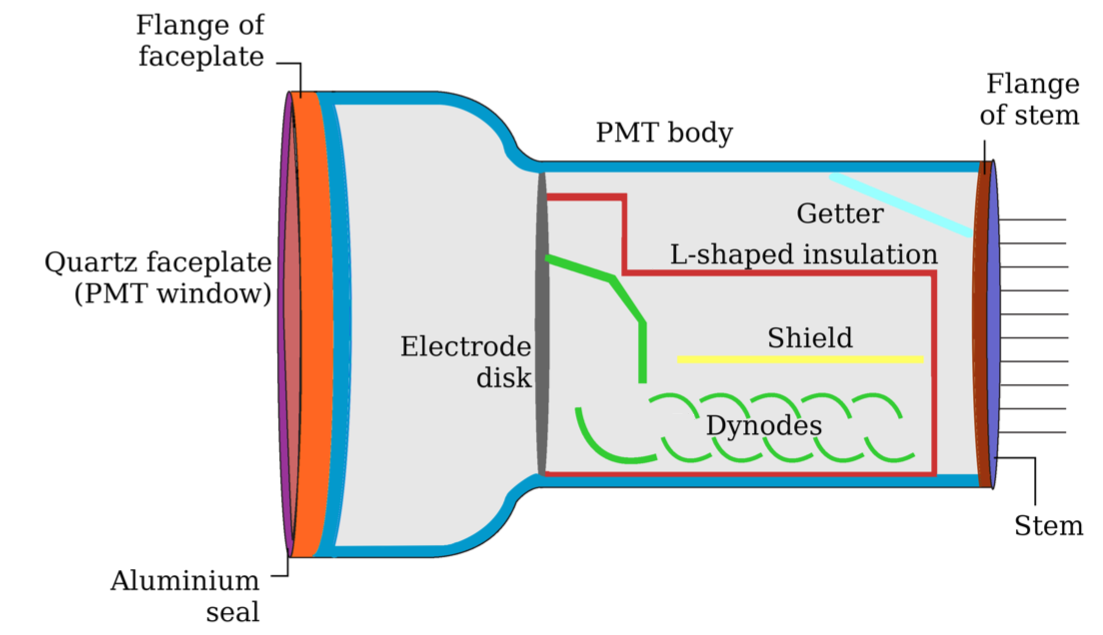
\includegraphics[width=0.8\textwidth]{PMTSchematic}
\caption{Schematic of the Hamamatsu R11410-21 PMT.  Image credit: \citeref{Aprile2015}.}
\label{fig:xenon1t_hamamatsu_pmt}
\end{figure}

The R11410-21 has 12 dynodes following a focusing electrode disk.  The first dynode is the largest and extends to the electrode disk to
maximize the probability of capturing photoelectrons.  A schematic can be be seen in \figref{fig:xenon1t_hamamatsu_pmt}.  The electrode,
dynodes, and shield are stainless steel and are insulated with L-shaped quartz plates.  Due to quartz's transparency to vacuum
ultraviolet (VUV) photons the window is also made of quartz.  Deposited on it is a low-temperature bialkali
photocathode.  The window is fixed with an aluminum seal to the faceplate flange, which along with the stem flange is constructed from
Kovar.  The body of the PMT is approximately 115 mm long and 35\% of the total mass.  It is constructed from Kovar alloy, most of which
has a very low \ce{^{60}Co} concentration.  Finally, to insulate the connections to each dynode the stem is ceramic.

Because radioactivity limits the fiducial volume and increases the event rate, making accidental coincidence and outlier events more
likely, XENON and Hamamatsu worked together to develop a highly radio-pure PMT.  The original R11410 version used ceramic as a dynode
insulator, standard Kovar alloy, and
purity aluminum for the seal.  Upgrading to quartz for the insulator, low-cobalt Kovar alloy, and high purity aluminum helped alleviate
this to an extent.  For the R11410-21 nearly all the \ce{^{137}Cs} and \ce{^{60}Co} comes from the Kovar alloy, though the \ce{^{137}Cs}
content is negligible and the \ce{^{60}Co} is 3-10 times lower than older models.  The decay rates of the remaining screened isotopes,
\ce{^{238}U},
\ce{^{228}Th}, \ce{^{228}Ra}, \ce{^{226}Ra}, and \ce{^{40}K}, are dominated by the ceramic stem (\citeref{Aprile2015}).  Unfortunately a
material that is more radio-pure and can insulate the dynode connections has not been found.  Sapphire was used in an iteration but
ultimately showed the reduction in background was minimal.

The number of signals per second without a light source is known as the dark count rate.  At ambient temperatures they
are primarily caused by thermal electrons and scale with PMT voltage.  This becomes subdominant at
cryogenic temperatures to electron field emission and radioactivity (internal and external) as well as cosmic rays.  Higher dark count
rates make accidental coincidence - when a lone-S1 and lone-S2 imitate a real event (\secref{subsec:backgrounds_ac}) - more likely.  The
fake additional background is dangerous because it can place false events in the signal region.  Because the rate is dependent on the
value above which events are recorded, known as the threshold, it can be tuned.  However, because
for DM searches we would like as low of a threshold as possible, choosing PMTs with low dark count rates is essential.

Another problematic feature is photon emission from the phototube itself, where light is created inside the PMT and escapes through the
window.  It has been observed to mainly occur in one of two ways.  The first is through a discharge of intense light that can last for
several seconds.  This ``flash" is easily bright enough to be observable to itself and by PMTs facing its
window.  However, the intensity can be so strong that it can take anywhere from several minutes to several hours for them to
recover.  Because they seem to happen spontaneously and are not well understood it is impossible to predict when a flash will occur.

The second process is an (often continuous) stream of light.  Known as ``micro light emission" it is considerably harder to
identify.  Doing so requires facing two phototubes towards one another and measuring the dark count rate of each with and without the
other
on.  The level of emission increases with temperature and bias voltage.  Keeping PMTs at cryogenic temperatures reduces
the frequency, and voltages can be lowered to help further.  Still, if micro light emission continues the PMT cannot be used as it risks
introducing fraudulent light into signals from events observed by other PMTs.

Directly following the pulse of a PMT hit a secondary pulse may occur.  Known as afterpulses, they can occur within tens of nanoseconds to
$\lesssim 5\ \mathrm{\mu s}$.  This can make them difficult or impossible to resolve from true pulses - especially S2s - that can have
widths of several
microseconds.  Because they are an inevitable side effect of PMTs it is important to carefully characterize them.

There are three mechanisms known to cause afterpulses.  The first is elastic scattering of the photoelectron with the first dynode,
freeing electrons that quickly return to the dynode, producing a second, smaller electron avalanche.  This
creates afterpulses in the range of a few to tens of nanoseconds.  A second kind is thought to come
from dark noise and single electrons but is not well understood.  It has a relatively uniform distribution in delay time up to several
microseconds.  Both of these afterpulses have relatively small areas of $\lesssim 2\ \mathrm{PE}$.

The third mechanism is a photoelectron may occasionally ionize residual gas inside the PMT along its trajectory to the first dynode.  The
ion then drifts
to the photocathode, where it expels additional electrons.  The number of newly ejected electrons (area of afterpulse) depends
on the ion and position where it was ionized.  The responsible ion can be determined by calculating the time between the true pulse and
afterpulse.  For the R11410-21 PMT this gives

\begin{equation}
\delta t_{\mathrm{ap}} = \frac{\pi}{4} \sqrt{\frac{2 m}{q V_{0}}} L
\end{equation}

\noindent where $\delta t_{\mathrm{ap}}$ is the afterpulse delay time, $m$ and $q$ are the ion's mass and charge, and $V_{0}$ and $L$ are
the potential
difference and length between the photocathode and first dynode (see \citeref{Barrow2017} for details).  Note that $\delta t_{\mathrm{ap}}$
does not depend on where the ionization occurred.  Therefore, if we know the time between the true and afterpulse the ion - or more
specifically
charge to mass ratio - can be determined.  $\delta t_{\mathrm{ap}}$ ranges from several hundred nanoseconds to several
microseconds and are shown in \figref{fig:xenon1t_pmts_ap}.  The prominent ions are highlighted.  The afterpulse delay time makes it
unlikely to couple with S1s but will do so for S2s.

\begin{figure}
\centering
\includegraphics[width=\textwidth]{afterpulse_spectrum_pmt_21}
\caption{Afterpulses for a PMT from XENON1T.  \ce{He^+}, \ce{CH_4^+}, \ce{N_2^+}, \ce{Ar^+}, and single- and double-ionized
xenon are present and marked by red lines.  The large fraction of Xe suggests a leak may be present, but to confirm should be monitored
over time to look for an increase in \ce{Xe^+} and \ce{Xe^{++}}.  If this is the case afterpulsing may hit a critical value at which point
the PMT can no longer dependably operate.  The second mechanism that can produce afterpulses in the text is visible as the roughly uniform
distribution at ${\sim}0.5\ \mathrm{PE}$.}
\label{fig:xenon1t_pmts_ap}
\end{figure}

Because it is not possible to eliminate all residual gas every PMT suffers from some ionization-based afterpulsing, as shown in
\figref{fig:xenon1t_pmts_ap} for one of the highest afterpulse PMTs.  A better vacuum
corresponds to fewer afterpulses and a ``healthier'' PMT.  If the concentration of gas in the PMT vacuum were to increase
it would
escalate the afterpulse rate.  Therefore if the Xe peaks grow over time the PMT likely has a leak and should
be replaced if possible, as continued worsening of the vacuum will lead to deterioration and eventually inability to operate the
PMT.  For XENON1T there are enough PMTs that replacement is not necessary.  All PMTs were tested before
installation.  73 were rejected and replaced: 12 due to high dark count rates, 53 for light emission, and 8 for
afterpulsing.

The transit time (TT) is the time between the photoelectron emission and the arrival of the electron avalanche at the anode.  Changes in
the photoelectron's initial position as well as emitted velocity and angle produce variation in the TT, which is characterized by the
transit time spread (TTS).  Because generally many PMTs observe an event the TTS quantifies how close together there signals should
be.  Thus
smaller TTSs lead to a smaller integration window, decreasing accidental coincidence.  The TTS for R11410-21 PMTs was measured, giving
a mean of $9.1 \pm 1.3\ \mathrm{ns}$ - or nearly the same as the digitizer rate.

The probability of double photoelectron emission (DPE) in a number of PMTs including the R11410 is between 0.18-0.24 - much higher
than previously thought (\citeref{Faham2015}).  For The R11410 in particular the probability was measured to be
$p_{\mathrm{dpe}} = 0.225 \pm 0.01$.  Any $p_{\mathrm{dpe}} > 0$ affects a number of elements in a DM
search.  In the past the expected value was low enough that it was not a major concern - however, at high values it cannot be
ignored.  First it may be useful to define a second quantity closely
related to but not the same as the QE.  Following \citeref{Faham2015} the QE will be denoted as $\eta_{\mathrm{\mu}}$ and the fraction of
incident photons that produce one or more photoelectrons denoted $\eta_{\mathrm{p}}$.  Then they are related by

\begin{equation}
\eta_{\mathrm{\mu}} = (1 + p_{\mathrm{dpe}}) \eta_{\mathrm{p}}
\label{eq:xenon1t_pmts_dpe}
\end{equation}

\noindent so using the measured QE alone is incorrect.  For one, it is common to require a PMT coincidence for an event to
be considered good - that is, $n$ PMTs must see a signal of a certain size within a predetermined time window.  Using
$\eta_{\mathrm{\mu}}$ will
\textit{overestimate} the likelihood of this happening, and $\eta_{\mathrm{p}}$ should instead be used.  Additionally, when the PMT
response is easily over threshold DPEs produce to incorrect resolution and yields unless accounted for.  Details on how to appropriately
account for $p_{\mathrm{dpe}}$ are in the electronic and nuclear recoil band fitting
(\secref{subsubsec:er_nr_calibrations_parameter_determ_det_phys}).

The two PMT arrays are supported by oxygen-free high thermal conductivity (OFHC) copper, with holes in which the PMTs are placed
(\figref{fig:xenon1t_pmt_array}).  The
copper is covered with polytetrafluoroethylene (PTFE) panels on the TPC-facing side.  Screening meshes are situated between the bottom
array and cathode as well as the anode and top array.  Each can be biased to minimize electrical interference between the
phototubes and the drift or extraction fields.  While \citeref{Baudis2013} showed normal operation of R11410 PMTs at
$\geq 11\ \mathrm{kV\ cm^{-1}}$ the anticipated cathode voltage was $10 \mdash 100\ \mathrm{kV\ cm^{-1}}$.  Installing the screening
meshes decreased stress on the phototubes and is expected to extend their life.

An additional six Hamamatsu R8520 PMTs reside in LXe outside the TPC near the top electrode for studying calibrations.  This model has
been used in a number of LXe TPCs including the PMT arrays in XENON100, and an electronic recoil measurement at
Columbia (\citeref{Goetzke2017}, \citeref{Aprile2012a}).




\subsection{TPC}
\label{subsec:xenon1t_tpc}
The XENON1T time projection chamber is a cylinder 96.9 cm in height and 95.8 cm in diamater and encloses a target mass of 2.0 tons.  A
(\figref{fig:xenon1t_tpc_tpc}).  The interior of the wall consists of 24 PTFE panels that were treated with diamond tools to
maximize VUV reflectivity, which increases the light collection efficiency.  Each interlocks with adjacent panels to achieve
light-tightness and the system is designed so that despite
the high thermal expansion coefficient the radius does not contract when lowered to $-96^{\circ}\mathrm{C}$.  Outside the PTFE are 74
field shaping rings made of low-radioactivity OFHC copper, each with a cross section of ${\sim} 10 \times 5\ \mathrm{mm^{2}}$.  They are
supported by 18 PTFE pillars stationed around the circumference.  Two redundant
chains connect adjoining rings via $5\ \mathrm{G \Omega}$ resistors and a $25\ \mathrm{G \Omega}$ resistor between the bottom ring and
cathode (\citeref{Aprile2017b}).

\begin{figure}
\centering
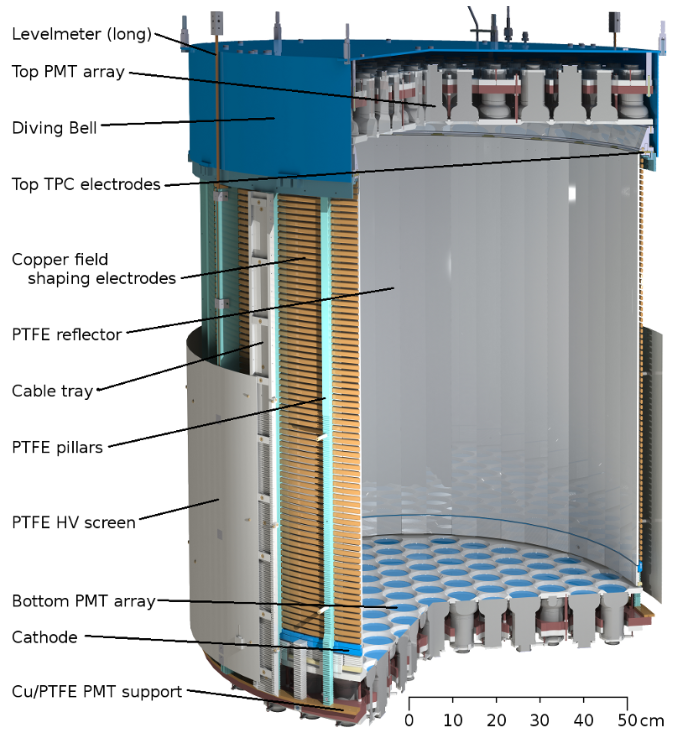
\includegraphics[width=0.8\textwidth]{XENON1TTPC}
\caption{Schematic of the TPC.}
\label{fig:xenon1t_tpc_tpc}
\end{figure}

There are five TPC electrodes that control the electric fields: the cathode, gate, anode, and top and bottom screening meshes.  They have
wired diameters of $\mathcal{O}(100)\ \mathrm{\mu m}$ and were designed to maximize light collection.  The cathode is connected to a
PNC150000-1 NEG high voltage supply and pre-filling tests successfully reached voltages beyond $-100\ \mathrm{kV}$.  48
mm below the cathode is the bottom screening mesh (mentioned in \secref{subsec:xenon1t_pmts}).  The mesh is 12 mm above the bottom PMT
array and can be biased to reduce unwanted effects from the PMT and cathode electric fields.  The cathode and bottom screening mesh
consist of
parallel wires and are gold-plated stainless steel to increase the workfunction.  The gate rests just below the
liquid-gas interface and defines $z = 0\ \mathrm{cm}$.  The anode is
situated 5 mm above the gate and is connected to a CAEN A1526P unit.  The last electrode is the top screening mesh 58 mm above
the anode and 11 mm below the top PMT array, and serves the same function is the same as the bottom mesh.  The top three electrodes are
made of stainless steel and are hex-etched.  Details for each electrode can be seen in
\tabref{tab:xenon1t_tpc_electrodes}.  \figref{fig:xenon1t_tpc_efield} shows the simulated electric field for the settings during the first
science run, Science Run 0.

\bgroup
\def\arraystretch{1.2}
\begin{table}
\centering
\resizebox{\textwidth}{!}{
\begin{tabular}{cccccc}
\hline
\hline
Electrode & Type & Diamater & Material & Transparency & Position \\
\hline
Top screening & hex meshed & $178\ \mathrm{\mu m}$ & stainless steel & 96.5\% & 63 mm \\
Anode & hex meshed & $178\ \mathrm{\mu m}$ & stainless steel & 89.8\% & 5 mm \\
Gate & hex meshed & $127\ \mathrm{\mu m}$ & stainless steel & 92.7\% & 0 mm \\
Cathode & parallel wires & $216\ \mathrm{\mu m}$ & gold-plated stainless steel & 97.2\% & -969 mm \\
Bottom screening & parallel wires & $216\ \mathrm{\mu m}$ & gold-plated stainless steel & 97.2\% & -1017 mm \\
\hline
\hline
\end{tabular}
}
\caption{Properties for TPC electrodes.  The cathode and bottom screening mesh have high transparency to optimize S1 light collection and
are gold-plated to decrease the risk of photoionization.}
\label{tab:xenon1t_tpc_electrodes}
\end{table}

\egroup

\begin{figure}
\centering
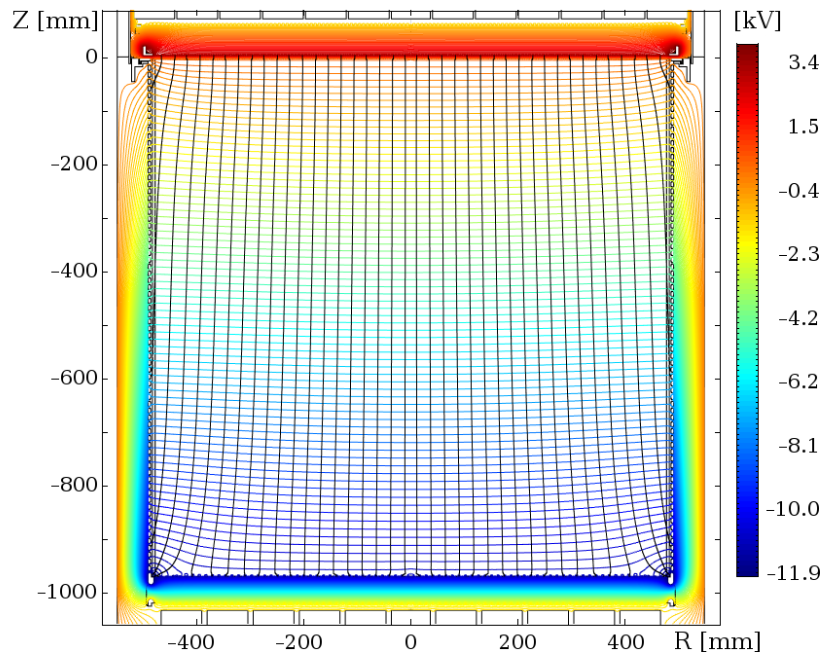
\includegraphics[width=0.8\textwidth]{ElectricField}
\caption{Finite element (COMSOL Multiphysics) simulation for the E-field inside and around the TPC.  Field and equipotential lines are
shown.  The voltages for the cathode, gate, and anode are $-12$, 0, and 4 kV, respectively - the settings for Science Run 0.  The field
is mostly uniform throughout the detector, which helps minimize biases that come from recombination, impurity attachment, etc.  Image
credit: \citeref{Aprile2017b}.}
\label{fig:xenon1t_tpc_efield}
\end{figure}

Four parallel-plate capacitors measure the liquid level.  They have a range of 10 mm with $30\ \mathrm{\mu m}$ precision and can be used
for measuring tilts or raising (lowering) the TPC.  The liquid level's height is adjustable through a gas-exhaust tube and maintained
with a ``diving bell" where controlled gas flow from purification pressurizes the GXe inside the TPC.  Two cylindrical levelmeters
with a 1360 mm range extend from the bottom PMT array to above the diving bell and are used during filling and recovery.  Placed around
the field cage are cable trays that power and transfer signals from the PMTs and temperature sensors.  They are made of PTFE and the
cables are held in place by PTFE spacers (\textbf{check if spacers is right word}).



\subsection{Cryogenic System}
\label{subsec:xenon1t_cryo}
The TPC is situated in the center of the water Cherenkov detector (\secref{subsec:xenon1t_water_shield}) and encompassed by the inner
cryostat.  Because the cryostat is in direct contract with xenon it is made of stainless steel and electropolished to reduce radon
emanation (\secref{subsubsec:backgrounds_electronic_radon}).  It is 1,960 mm tall by 1,100 mm diamater and is metal-sealed
using a Helicoflex seal.  Surrounding it is the 2,490 mm tall by 1,620 mm diamater outer cryostat separated by vacuum.  It is also
constructed from stainless steel but
because there is no contact with xenon electropolishing is unncessary.  The two are thermally isolated by Torlon polyamide-imide spacers
and vacuum.  Heat loss is further mitigated to ${\sim} 75\ \mathrm{W}$ by aluminized mylar foil wrapped around the inner
vessel.  Materials were screened prior to construction for
radioactivity.

A 10 m high stainless steel support structure was built inside the water tank.  Attached are three M20 rods that suspend the
cryostat.  They can be adjusted independently to customize the inclination of the LXe level with respect to the
TPC.  A chain secures the bottom of the outer vessel to the water tank floor to counteract buoyancy forces when the cryostat is empty.  A
double-walled pipe with inner and outer diameters 254 and 406 mm, respectively, connects with purification (\secref{subsec:xenon1t_pur}),
cooling,
pressurization for the diving bell, and emergency recovery, and carries the PMT and auxiliary cables.  A separate pipe connects the
cathode with the outside.  A schematic of the cryostat is shown in \figref{fig:xenon1t_cryo_cryostat_diagram}.

\begin{figure}
\centering
\includegraphics[width=0.8\textwidth]{cryo_diagram}
\caption{Diagram of the cryostat.  Image credit: \citeref{Aprile2017c}.}
\label{fig:xenon1t_cryo_cryostat_diagram}
\end{figure}

A total of 3.5 tons of xenon is stored in the cryostat.  In addition to the 2.0 t of LXe inside the TPC, 1.5 t is between the
TPC and inner vessel.  The mass of the GXe is ${\sim} 20 \mdash 30\ \mathrm{kg}$.  The nominal LXe temperature is
$T_{0} = -96^{\circ}\ \mathrm{C}$.  Gas near the top of
the cryogenic system is liquified by pulse-tube refrigerators (PTRs) into a funnel and flows down to the TPC through a pipe to be
deposited in the inner vessel beneath the TPC.  Because
the PTRs are higher than the TPC the flow is guided by gravity.  \figref{fig:xenon1t_cryogenics_schematic} shows the layout of the
cryogenic
system.  The cryogenic system extends from the TPC into a service building outside the water tank through a long tube known as the
neck.  The two PTRs occupy independent
cooling towers and can each deliver $250\ \mathrm{W}$ of cooling power.  With the xenon
having a total thermal load of ${\sim} 150\ \mathrm{W}$ only one needs to be active at any time.  The cooling towers
are located in the service building.  Each PTR connects to a copper coldfinger
inside the inner cryostat so they can be removed without exposing the xenon to air.  A proportional-integral-derivative (PID) controller
monitors and adjusts the temperature of a resistive heater on the coldfinger to maintain stable pressure.

A third cooling tower (also in the service building) uses liquid nitrogen ($\mathrm{LN_2}$) and is used in an emergency, if both PTRs are
being serviced, or the
heat load becomes too great from e.g. loss of power or insulation vacuum.  The $\mathrm{LN_2}$ flows from a $10 \mathrm{m^3}$ tank that
is also used by ReStoX (\secref{subsec:xenon1t_restox}).  The cooling power can regulated by adjusting the $\mathrm{LN_2}$ evaporation
rate.  In the event the PTRs
lose power the $\mathrm{LN_2}$ cooling tower must react immediately to prevent rising pressure that can damage PMTs and other
components.  Sensors and controllers monitoring such a power loss are connected to uninterruptible power supplies (UPSs) to ensure a
successful transition and operation of $\mathrm{LN_2}$.

\begin{figure}
\centering
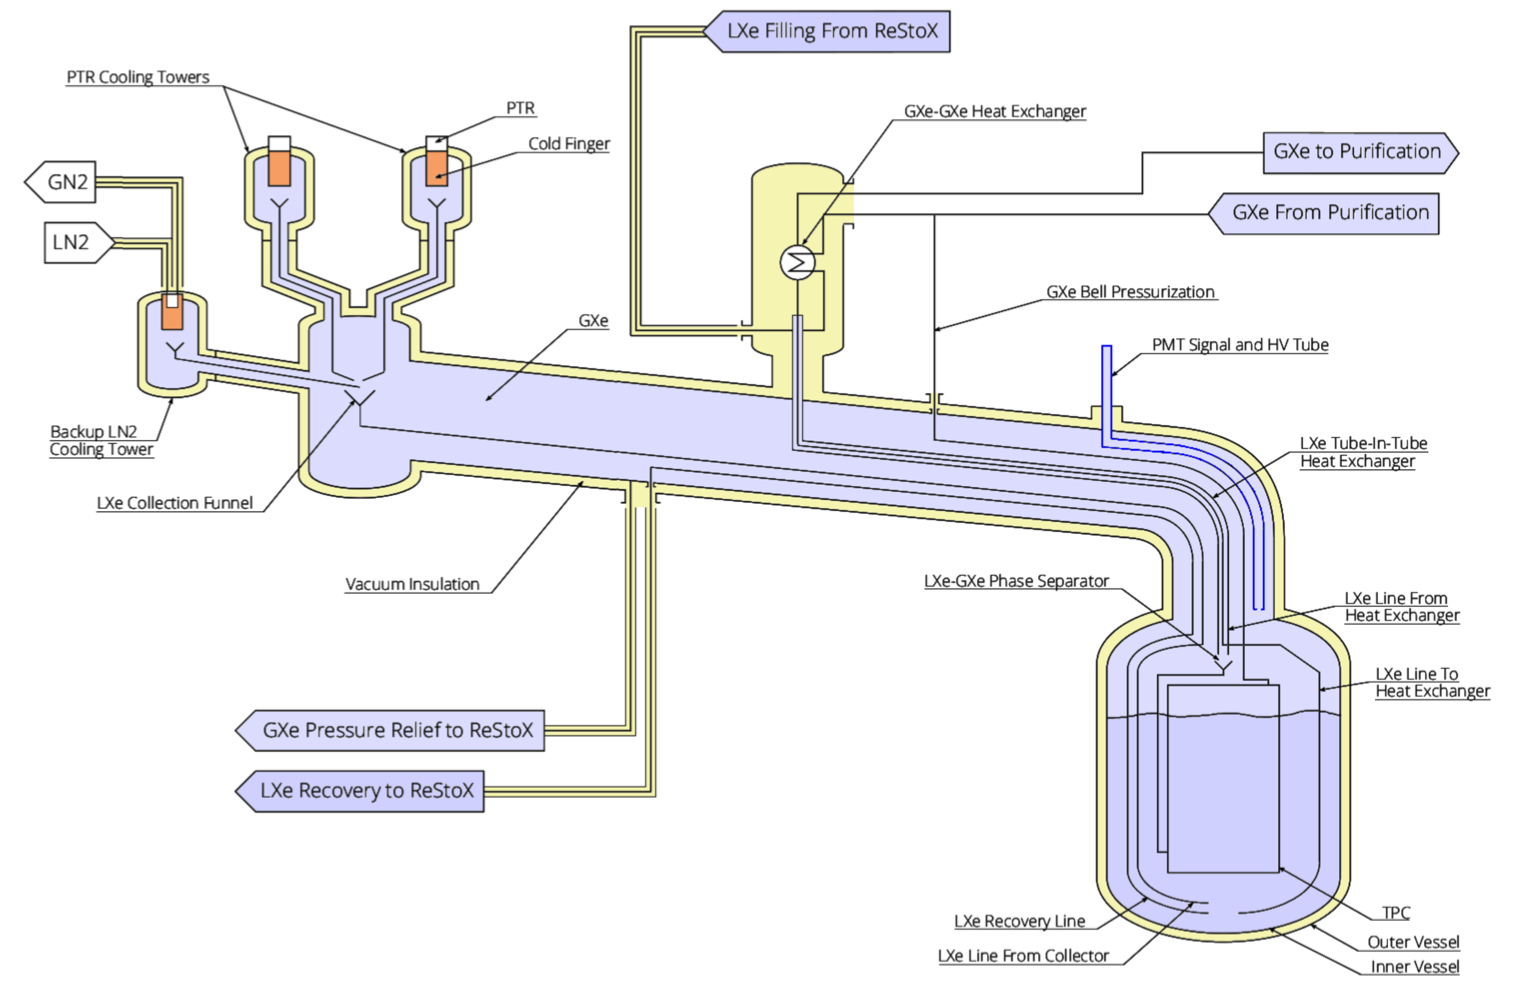
\includegraphics[width=\textwidth]{CryostatSchematic}
\caption{Layout of the cryogenic system.  Three cooling towers - two with PTRs and one backup $\mathrm{LN_2}$ - liquify GXe that returns
to the TPC.  LXe is carried from the bottom of the cryostat to the purification system (\secref{subsec:xenon1t_pur}) through a heat
exchanger system, while
returning xenon flows into the bottom of the TPC with excess gas diffusing into the GXe.  A portion of purified GXe is extracted
before the heat exchanger and used to maintain pressure inside the diving bell.  Connections with ReStoX (\secref{subsec:xenon1t_restox})
are also shown.  Image credit: \citeref{Aprile2017b}.}
\label{fig:xenon1t_cryogenics_schematic}
\end{figure}

Connections to purification and ReStoX are shown in \figref{fig:xenon1t_cryogenics_schematic}.  LXe from the beneath the TPC is removed
for purification.  It passes
through a two-phase heat exchanger system, whose purpose is to guide the exchange of thermal energy between GXe returning to the TPC
and LXe leaving.  The returning xenon is cooled before it reaches the TPC, and likewise removed xenon is heated before
the purification.  The first step of the system is the ``tube-in-tube" component where two concentric tubes carrying LXe (GXe) away from
(towards)
the TPC.  The second component is a plate heat exchanger and is closer to the purification system (i.e. returning xenon passes through
before tube-in-tube).  The system is extremely efficient and significantly reduces the required cooling power that would be necessary
without it.

The heat exchange
efficiency $\epsilon$ is the fraction of heat necessary for temperature change and vaporization that stays outside of the system.  A
higher
efficiency means better thermal energy transfer between the GXe and LXe and decreases the heat load on the system.  This is
because instead of GXe entering the cryostat at roughly
room temperature, it returns at approximately that of LXe with much of it having liquified, putting less stress on the
PTRs.  An essential ingredient of the heat transfer is the latent heat, which comprises ${\sim} 80\%$ of the total exchange.  The
difference in vaporization temperature of the outgoing xenon and condensation temperature of incoming xenon is

\begin{equation}
\Delta T_{\mathrm{ph}} = T_{\mathrm{gl}} (P_{\mathrm{i}}) - T_{\mathrm{gl}} (P_{\mathrm{o}})
\label{eq:xenon1t_cryo_latent}
\end{equation}

\noindent where $T_{\mathrm{gl}} (P)$ is the pressure-dependent temperature of the gas-liquid phase transition, and $P_{\mathrm{i}}$ and
$P_{\mathrm{o}}$
are the pressures of the incoming and outgoing xenon, respectively.  Because the conditions of the dynamical gas flow
(\secref{subsec:xenon1t_pur}) cause $P_{\mathrm{i}} > P_{\mathrm{o}}$, $\Delta T_{\mathrm{ph}} > 0$, making it effective at heat transfer
(\citeref{Aprile2012b}).  A study with the Demonstrator - the
experiment used to for research and development for XENON1T (\secref{subsec:electron_lifetime_model_demonstrator}) - showed a heat
exchange efficiency for
two heat exchangers in series of $\geq 96\%$ (\citeref{Aprile2012b}).  Following the parallel-plate exchanger a heater provides additional
thermal energy to the xenon moving towards the purification system.  The different systems that handle the xenon can be seen in
\figref{fig:xenon1t_cryo_overview}.

\begin{figure}
\centering
\includegraphics[width=\textwidth]{cryo_overview}
\caption{The various systems that handle xenon in the experiment: cryostat, cryogenics, purification, cryogenic distillation column,
ReStoX, bottle racks, and gas analytics station.  The water shield flange defines the region between the service building and the water
Cherenkov detector.  Image credit: \citeref{Aprile2017b}.}
\label{fig:xenon1t_cryo_overview}
\end{figure}



\subsection{Purification}
\label{subsec:xenon1t_pur}
LXe contamination presents number of problems.  As mentioned in \secref{subsec:tpcs_working_principle} electronegative
impurities (e.g. O$_2$, H$_2$O, N$_2$O, etc.) will attach to drifting $e^-$, reducing the number that reach
the liquid surface and thus the S2.

Impurities will also attenuate scintillation, which pushes our energy threshold up as fainter signals become harder to detect.  This is
described by

\begin{equation}
I(x) = I_0 e^{-x / \lambda_{\mathrm{att}}}
\label{eq:xenon1t_pur_atten}
\end{equation}

\noindent where $I_0$ is initial number of photons, $I(x)$ is the number after traveling a distance $x$, and $\lambda_{\mathrm{att}}$ is
the
attenuation length.  $\lambda_{\mathrm{att}}$ is dependent on the absorption and scatter lengths, $\lambda_{\mathrm{abs}}$ and
$\lambda_{\mathrm{scat}}$.  The absorption length describes the true loss of photons while the scatter refers to photons that elastically
scatter without energy loss.  This is covered in greater detail in \secref{subsec:importance_procedure_effects_photons}.

Electronegative impurities come primarily from outgassing of detector materials.  They are measured in O$_2$-equivalent - that is, the
analogous concentration of oxygen if it
were the only contaminant.  For LXe experiments the necessary concentration is 1 part per billion (ppb) or less.

In addition
to the GXe from the TPC (after passing through heat exchanger and heater as described in \secref{subsec:xenon1t_cryo}), connections are
made between
each of the cooling towers and the purification system.  Because impurities are lighter than xenon they are anticipated to have a larger
presence in the gas.  While the GXe impurity concentration has no direct effect on \electron loss, impurities will migrate between the
LXe and GXe.  Purifying the GXe should largely reduce the impurities that pass into the liquid.

Xenon from ReStoX  (\secref{subsec:xenon1t_restox}) and bottles are also connected to the purification system.  A separate heat exchanger
sits between ReStoX and purification.  In
addition to cleaning the Xe as it is transfered from ReStoX to the cryostat, the purification system connects ReStoX to the Kr
distillation column (\secref{subsec:xenon1t_kr_dist}).  The column returns the xenon after distillation to purification.  All systems that
feed into the purification system do so before the getters and are available as outputs as well.  A small tube between the purification
and cryostat before the heat exchanger siphons GXe to pressurize the bell to maintain the liquid level, and is regulated by a flow
controller.  The numerous connections makes the purification system a hub for transferring xenon between systems.

\begin{figure}
\centering
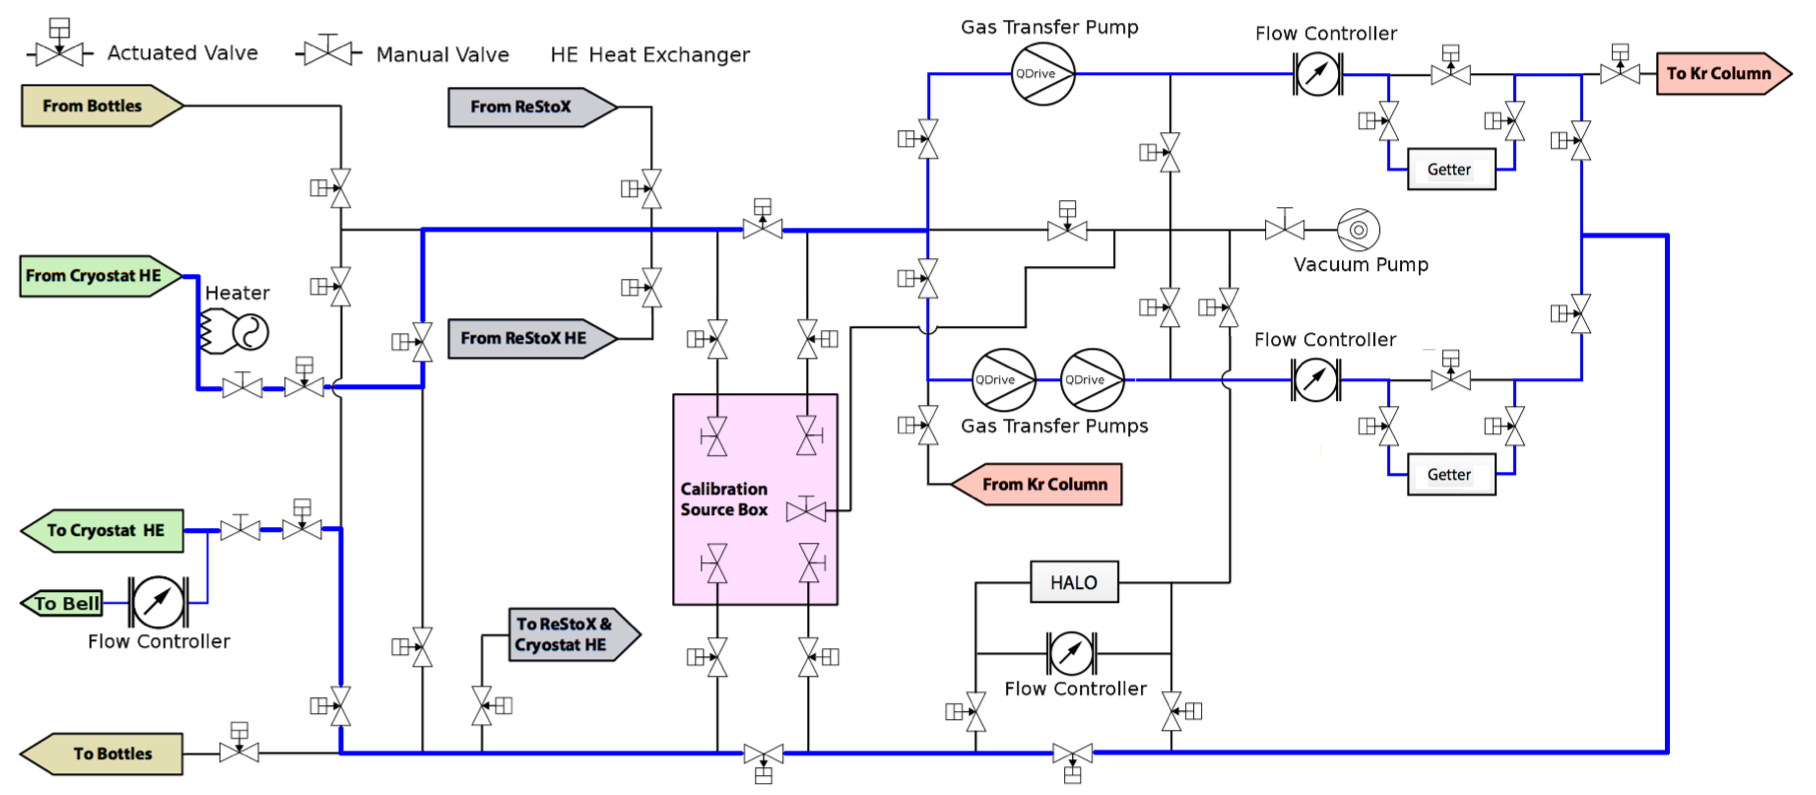
\includegraphics[width=\textwidth]{PurificationLayout}
\caption{Layout of the purification system.  The standard flow path during normal operations is highlighted in blue.  Image credit:
\citeref{Aprile2017b}.}
\label{fig:xenon1t_pur_schematic}
\end{figure}

The purification system consists of two redundant purification loops, each of which can operate independently of the other.  The flow
is driven by CHART QDrives, with one in one loop and two in the other.  They were chosen for their high-capacity and hermetically sealed
pump volume, the latter of which was not true with KNF pumps that were used in XENON100 (\textbf{check this}).  This is important because
exposure to air could cause a significant drop in purity, and has occurred in the past with KNFs.  They are
magnetically-resonant and operate via a compression space with oscillating externally-driven pistons.  Motors, valves, and pistons are
not lubricated, making it an excellent choice for high-purity.  Unfortunately QDrives emanate \ce{^{222}Rn} and can require frequent
maintenance if operated at too great a voltage (for larger flow).  For the former, \ce{Rn} emanation measurements were made prior to
installation and the pumps with the lowest concentrations were selected.  For the latter they are operated at safe conditions and since
the beginning of Science Run 0
no issues have arisen.  The limiting factor on circulation speed is not a result of the pumps but the pressure difference
from 1/2" outer diameter (OD) tubes leading to the system.  After Science Run 1 replacement 1" OD pipes were installed
(\secref{subsec:electron_lifetime_model_ops}).  One QDrive is installed in one loop and two in the other.

The flow of the GXe is maintained by two MKA 1579A mass-flow controllers - one on either branch.  The assumption before the experiment
went
online was these would limit the speed when necessary, but because we did not achieve our goal these have minimal impact.  Still, they can
be used for further restriction.  The xenon then passes through SAES PS4-MT50-R high-temperature rare-gas purifiers, or getters.  They
use heated ($400^{\circ}\mathrm{C}$) zirconium to form unbreakable bonds with carbide, nitride, and oxide, lowering the impurity content
to $< 1\ \mathrm{ppb}$ (\citeref{Aprile2017b}).  A bypass valve allows the xenon to pass un-purified in the event that the it does not
need to be cleaned.

A Tiger Optics HALO+ H$_2$O monitor measures the water content in the purified GXe to track the purification efficiency.  It can measure
concentrations down to 400 ppt.  As with the getters, it can be bypassed.  The Xe is then forwarded to the cryostat, bell, ReStoX, or
bottles (Kr column occurs after the purification loops before the HALO).

The components of the system are electropolished and able to be baked up to ${\sim} 120^{\circ}\mathrm{C}$ for decreased outgassing
(\secref{subsubsec:electron_lifetime_model_outgassing_sources}).  The purification system has a number of valves that allow the versatility described in this section.  The majority are
pneumatic and can
be operated remotely with the slow control system (\secref{subsec:xenon1t_detector_slow_control}).  The remainder are manual valves
situated in select locations: to and from the cryostat,
inside the calibration box, and before the vacuum pump, which can be used to evacuate individual sections or the entire system.  These are
in place as a precaution against accidental openings of the actuated valves.


\subsection{ReStoX}
\label{subsec:xenon1t_restox}
The Recovery and Storage system for XENON1T (ReStoX) stores xenon not in use by other systems.  It is located on the ground floor of the
service building.  With a volume of 4.95 m$^{3}$
(diameter of 2.1 m), wall thickness of 28 mm, and ability to withstand pressures of up to 73 bar, it can support 7.6 tons of
xenon
as a gas, liquid, or super-critical fluid.  It is made from stainless steel and insulated via vacuum from an outer sphere, where
thermal conductance is extremely low due to with superinsulation and limited contact to an external heat load of
${\sim}50\ \mathrm{W}$.  To limit
impurity contamination while the Xe is in ReStoX the vessel and valves are metal sealed and electropolished.

The xenon is cooled by 16 lines welded to the inner vessel's outer surface that carry LN$_2$ that from the 10 m$^3$ dewar adjacent to the
service building.  To prevent over-cooling 16 stainless steel fins inside increase heat
exchanging.  A condenser and heater in the middle are used when the xenon is stored as a liquid, which is normally the case.  The heater
ensures solid xenon does not obstruct pipes so Xe can be transfered freely with other systems.  The total cooling power of
$> 3\ \mathrm{kW}$ is spread over 4.3 m$^2$ of copper (\citeref{Aprile2017b}).

\begin{figure}
\centering
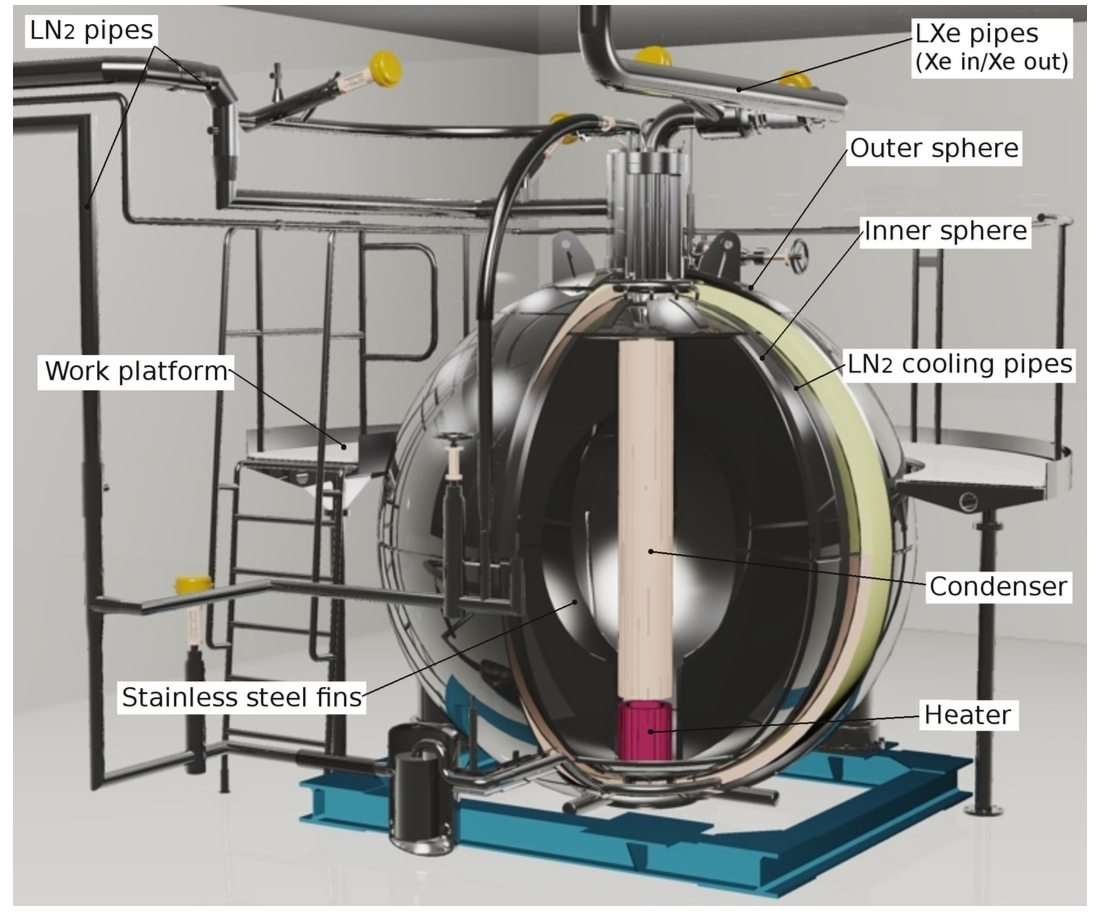
\includegraphics[width=0.8\textwidth]{ReStoX}
\caption{ReStoX with major components labeled.  Image credit: \citeref{Aprile2017b}.}
\label{fig:xenon1t_restox_pic}
\end{figure}

Previous LXe experiments would fill detectors by condensing the GXe from storage.  Similarly, recovery was done by allowing the LXe
in the cryostat to evaporate.  While this was feasible for detectors with $\mathcal{O}(100)\ \mathrm{kg}$ of xenon, doing so
(\textbf{maybe it is just for filling, check}) for XENON1T would require approximately two months, and fast recovery in the event of an
emergency would not be possible.  This is solved through the purification system, which as mentioned in \secref{subsec:xenon1t_pur} can
pump xenon between systems and significantly expedite the process (\textbf{check with someone about how xenon is recovered}).



\subsection{Krypton Distillation}
\label{subsec:xenon1t_kr_dist}
Commercial high-purity xenon generally has \ce{Kr} concentrations between 1 ppm to 10 ppb.  This is not clean enough for LXe dark matter
detectors so additional distillation is necessary.  The reason for restricting the
krypton content is \ce{^{85}Kr}, which has a half-life of 10.76 years and undergoes \betadecay with an end-point energy of 687 keV.  With
an expected fraction $\mathrm{^{85}Kr / ^{nat}Kr = 2 \times 10^{-11}}$ the required \ce{^{nat}Kr}/Xe concentration for its background to be
less than radon was expected to be $< 200\ \mathrm{ppq}$.  Details of the \ce{^{85}Kr} background can be found in
\secref{sec:backgrounds}.

To achieve this purity we use a Kr distillation column, seen in \figref{fig:xeno1t_kr_dist_column}.  The column has a total
height of 5.5 m and is kept in an insulation vessel at $10^{-5}\ \mathrm{mbar}$ to minimize thermal losses (\citeref{Aprile2016b}).  GXe
enters through a heat exchanger and is
liquified by the input condenser, which uses a cryo-cooler (Leybold CP-50) at $-98^{\circ}\mathrm{C}$ and maximal power
of 100 W.  Next it moves to the package tube, built with 2.8 m of structured stainless steel package material (Sulzer EX) 45 cm in
diamater that has feeding ports for both liquid and gaseous xenon.  At the top of the tube is a second cryo-cooler (Leybold CP-140T)
at $-98^{\circ}\mathrm{C}$ and capable of 200 W.  Liquified xenon will fall to the bottom, where it is stored and heated by a
reboiler with up to 300 W.  The Kr, with a lower atomic mass will drift towards the top of the column but will not liquify as its
boiling point is lower than $-98^{\circ}\mathrm{C}$.  Siphoning gas at the top removes Kr at a much higher concentration than
present in the inlet GXe.  The more pure Xe at the bottom is extracted where it passes through the heat exchanged before returning to the
purification system or ReStoX (\textbf{check this}).

\begin{figure}
\centering
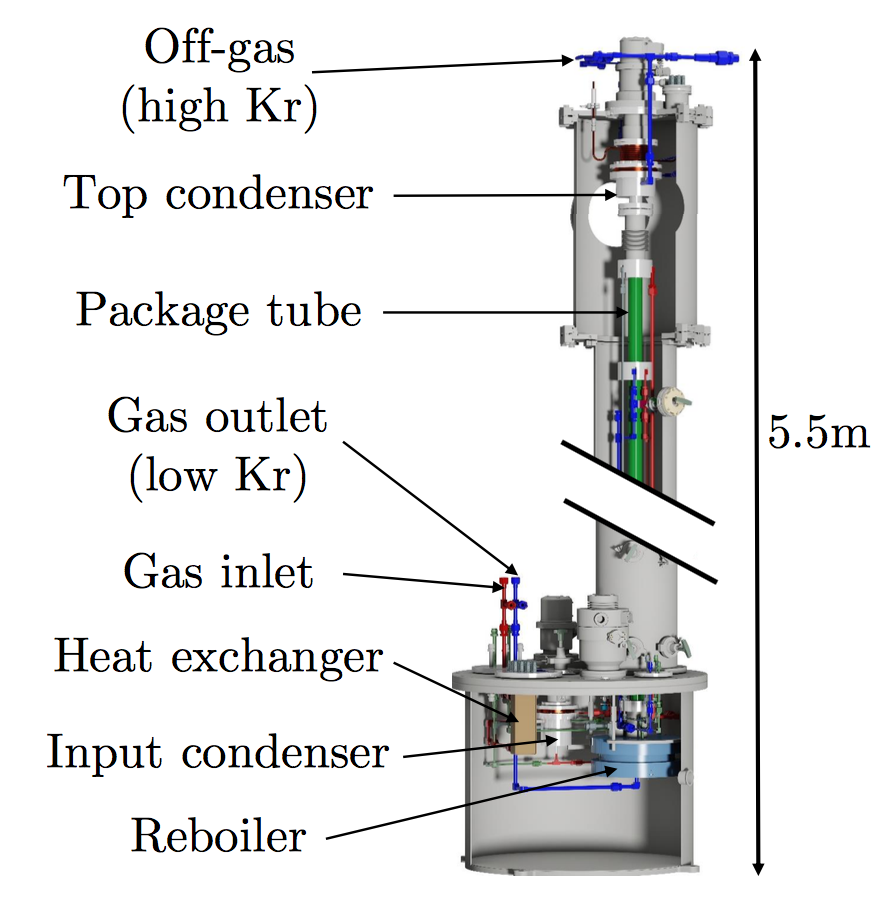
\includegraphics[width=0.6\textwidth]{KrColumn}
\caption{Image credit: \citeref{Aprile2017b}.}
\label{fig:xeno1t_kr_dist_column}
\end{figure}

Once installed at LNGS the reduction of \ce{^{nat}Kr}/Xe was found to be $6.4_{-1.4}^{+1.9} \times 10^{5}$
(\citeref{Aprile2016b}).  Inlet flows have been shown to be stable up to 18 slpm, but running all ReStoX xenon through distillation on the
way to the cryostat during filling would take ${\sim}3$ weeks.  For this reason an online removal system was used, where the xenon was
distilled during
science run data taking.  For over 70 days 7\% of xenon passing through the purification system was diverted to the column and a total
of 0.07\% was
removed.  An initial \ce{^{nat}Kr}/Xe concentration of 60 ppb was decreased to $360 \pm 60\ \mathrm{ppq}$, the lowest ever realized in a
LXe dark matter experiment.  Measurements of \ce{^{nat}Kr}/Xe are done using a rare gas mass spectrometer (RGMS) that uses cryogenic gas
chromotography to separate the Kr from Xe, followed by a mass spectrometer for Kr measurement (\citeref{Lindemann2014}).

The second most worrisome low-energy background comes from the \ce{^{222}Rn} decay chain.  While the distillation column was oirginally
built and intended for Kr,
it was shown to work in a single stage distillation (\citeref{Bruenner2017}) and subsequently XENON100
(\citeref{Aprile2017d}).  It operates using the reverse principle, i.e. radon-enriched xenon coalesces near the bottom of the column and
is extracted and stored in bottles, while the more pure xenon at the top is returned to the purification system.



\subsection{Water Shield}
\label{subsec:xenon1t_water_shield}
Limiting radiation from outside the experiment is essential to a dark matter search.  An active water Cherenkov detector encompasses the
cryostat, spanning 9.6 m in diamater and 10.2 m high.  It is filled with deionized water, which can fill the Cherenkov detector at up to
$2.2\ \mathrm{m^{3}\ h^{-1}}$.  The tank shields the cryostat from neutrons and \gammarays that originate underground (from e.g. rocks),
decreasing the number of events that reach the TPC by orders of magnitude.

84 Hamamatsu R5912ASSY PMTs are placed in five rings along the inner wall of the water tank, 2.5 m apart in height.  The lowest
($z = 0\ \mathrm{m}$) and highest ($z = 10\ \mathrm{m}$) rings each contains 24 PMTs, while the three between them have 12 each.  The
quantum efficiency for each PMT is ${\sim}30\%$ between 300-600 nm.  To increase the chance of photon detection the inner wall is coated
with foil (3M DF2000MA) that has
nearly 100\% reflectivity at $> 400\ \mathrm{nm}$, (\citeref{2017Geis}).  However, ${\sim}90\%$ of light is absorbed for
$<370\ \mathrm{nm}$ and 3-7.5\% from $250 \leq \lambda \leq 370\ \mathrm{nm}$ is wavelength shifted to more favorable values for the PMTs.

The purpose of the PMTs is to identify muons and muon-induced neutrons by detecting showers initiating
outside the water tank.  Using the difference in arrival times to each PMT the path of the particle can be reconstructed as shown in
\figref{fig:xenon1t_water_shield_photo}.  If an event in the TPC coincides with one in the water tank it is excluded.  For this reason
the system is referred to as the muon veto (MV).  The flux of muons at LNGS is $3.31 \pm 0.03 \times 10^{-8}\ \mathrm{cm^2\ s^{-1}}$ with
average energy ${\sim}270\ \mathrm{GeV}$ (\citeref{Aprile2017b}).

\begin{figure}
\centering
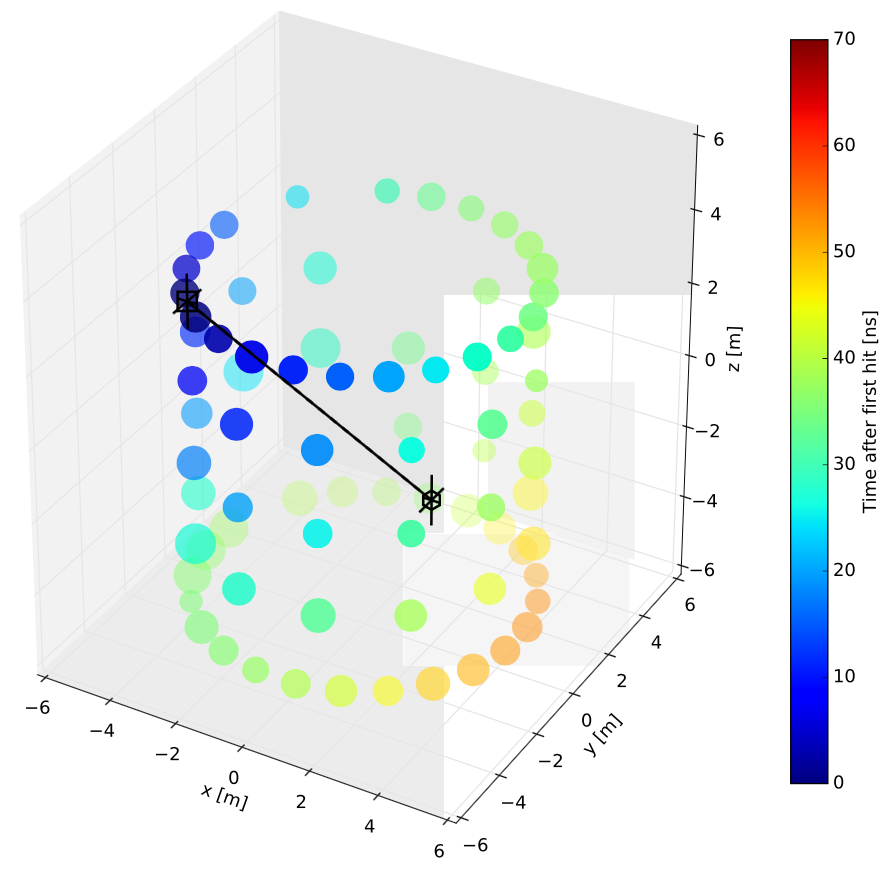
\includegraphics[width=\textwidth]{MuonVetoEvent}
\caption{Arrival time of light to muon veto PMTs helps reconstruct the muon trajectory (black line).}
\label{fig:xenon1t_water_shield_photo}
\end{figure}

\begin{figure}
\centering
\includegraphics[width=\textwidth]{InsideWaterTank}
\caption{Photo from inside the water tank during commissioning.  The muon veto PMTs can be seen around the perimeter covered in black bags
to shield them from the
light.  The neck of the cryogenics system extends through the hole in the back from the service building to the cryostat, with the
inner vessel wrapped in mylar visible beneath.}
\label{fig:xenon1t_water_shield_interior}
\end{figure}



\subsection{Calibrations}
\label{subsec:xenon1t_calibrations}
Calibrations are used for a host of purposes including understanding energy resolution, light collection efficiency, electron lifetime,
electronic and nuclear recoil bands, and many more.  Depending on the source they can be performed inside the TPC (internal)
or outside (external).  The different calibrations and the purposes they serve are discussed here; additional details and results are in
\secref{sec:det_char}.

\begin{figure}
\centering
\includegraphics[width=\textwidth]{panoramic_xenon1t}
\caption{The XENON1T experiment with the water tank (left) and service building (right).  A depiction of inside the water tank
hangs on the outside.  ReStoX (first floor), DAQ (second), and the cryogenic system (third) are visible in the service building.}
\label{fig:xenon1t_panoramic}
\end{figure}

\subsubsection{Internal}
\label{subsubsec:xenon1t_calibrations_internal}
Internal calibrations allow us to describe how our detector observes events throughout the entire TPC.  This is preferable to external
calibrations (\secref{subsubsec:xenon1t_calibrations_external}), where events are more focused in the section of the TPC near the
wall.  The calibration source box is installed in the
purification system (pink region in
\figref{fig:xenon1t_pur_schematic}) and contains valves opening to the GXe both before and after the
getters.  This is clearer in \figref{fig:xenon1t_pur_cal_box_schematic}, which shows a detailed schematic of the source box including
locations of $\mathrm{^{83m}Kr}$, \ce{^{220}Rn}, and \ce{CH_3T}, valves and filters, and connections to the purification system and
cryostat.  When the valves are opened,
the source will flow into the GXe stream and cryostat.  Therefore only sources that do not introduce
electronegative impurities are used.  The source will quickly diffuse in the xenon to become uniformly distributed,
allowing a number of detector characteristics and properties throughout the entire TPC to be studied.

$\mathrm{^{83m}Kr}$ has monoenergetic decays of 32.2 ($t_{1/2} = 1.83\ \mathrm{h}$) and 9.4 keV
($t_{1/2} = 154.4\ \mathrm{ns}$).  The short
half-lifes and its final decay product \ce{^{83}Kr} being stable and a noble gas make it a great choice to measure the light collection
efficiency (LCE), the electron lifetime, and many other important features.

\radoncal is used to calibrate the electronic recoil (ER) band as its progeny \ce{^{212}Pb} is a $\beta$-emitter with endpoint energy
569.91 keV.  There are other $\alpha$- and $\beta$-emissions throughout the chain that can be used for additional studies,
including measuring the electron lifetime with the \ce{^{212}Bi} $\alpha$-decay.  The longest half-life in the chain is
\ce{^{212}Pb} with $t_{1/2} = 10.6\ \mathrm{h}$ (next longest is \ce{^{212}Bi} with $t_{1/2} = 1.00\ \mathrm{h}$) so dark matter data
can resume within several days.

\begin{figure}
\centering
\includegraphics[width=0.8\textwidth]{calibration_source_box}
\caption{Layout of the calibration source box in the purification system.  Locations of \ce{^{220}Rn}, $^{83\mathrm{m}}\mathrm{Kr}$, and
\ce{CH_3T} are marked by dotted rectangles.  Filters are installed to catch debris.  Connections to and from the cryostat (turquoise)
and pumps and getters (red) are shown.  The vacuum pump (yellow) is used to evacuate the chamber before use.}
\label{fig:xenon1t_pur_cal_box_schematic}
\end{figure}

Tritiated methane ($\mathrm{C H_3 T}$) is a very attractive candidate because of it's low-energy $\beta$-emission.  With a 18.6 keV
endpoint energy, it is an ideal candidate for calibrating the low-energy ($\mathrm{cS1} < 60\ \mathrm{PE}$) ER band
and measuring
the light and charge yields in an important region.  This was originally done by LUX (\citeref{LUX2016}) and
subsequently performed with XENON100 (\citeref{Aprile2018}).  However, with a half-life of $t_{1/2} = 12.3\ \mathrm{y}$ it must be
removed completely by the getters because introducing a new background in the dark matter region of interest would be disastrous.  There
is a worry that
$\mathrm{C H_3 T}$ adheres to the cryostat, prohibiting complete removal.  For this reason a $\mathrm{C H_3 T}$ calibration has not
yet been conducted in XENON1T.

PMT gains are calibrated using blue LEDs at low light levels.  Unlike other sources this calibration is done using fiberoptic cables that
are
carried from the data acquisition (\secref{subsec:xenon1t_daq}) into the TPC.  They are fixed at various heights and angles to optimize
PMT calibrations and flash at periodic intervals.  They are used to measure the single photoelectron (SPE) spectrum
(\figref{fig:xenon1t_pmt_spe}) and PMT afterpulsing (\figref{fig:xenon1t_pmts_ap}).

\begin{figure}
\centering
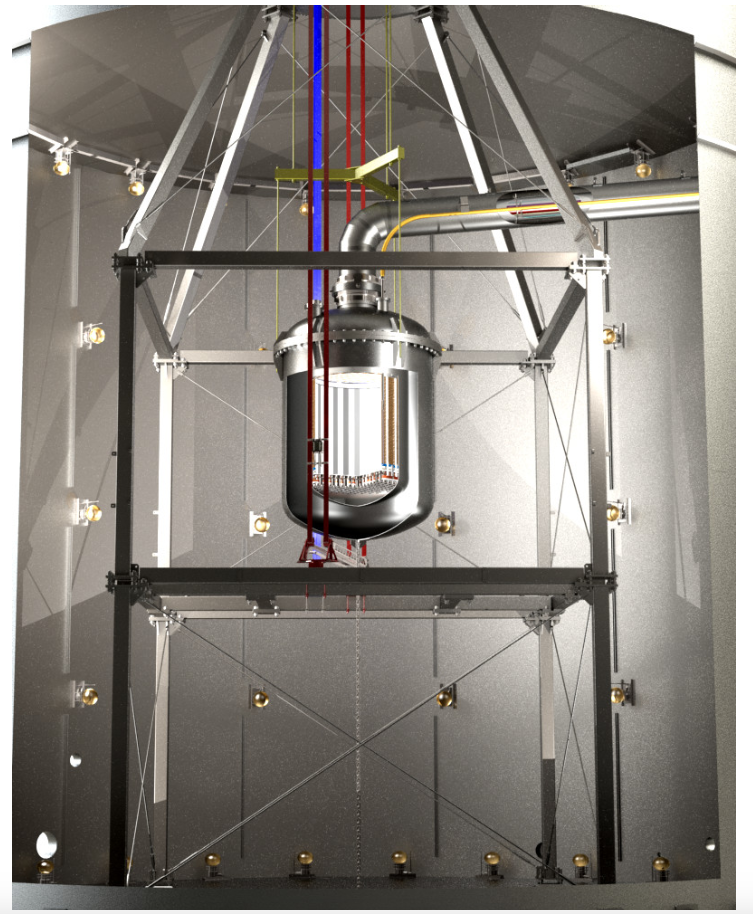
\includegraphics[width=\textwidth]{WaterTankInside}
\caption{Interior of the water tank.  The belts highlighted in blue, maroon, and red, and the portion of the U-belt that extends
underneath the cryostat is visible.  Six wires - three extending from the roof to the cross and three from the cross to the
cryostat - adjust the liquid level and are marked in dark yellow.  The connection from the service building to the cathode is shown in
bright yellow.  The chain fixes the cryostat to the floor of the water tank to counter buoyancy forces.  The large metal structure is the
skeleton from the below-ground clean room used while installing the TPC.  PMTs for the muon veto are attached to the water tank.}
\label{fig:water_tank_inside}
\end{figure}



\subsubsection{External}
\label{subsubsec:xenon1t_calibrations_external}
External calibrations are performed with the source outside the cryostat.  In XENON100 this was done by inserting a source inside the
protective lead
shielding; however, the size of the water tank in XENON1T requires the installation of two ``I-belts"
along the height of the detector and one ``U-belt" that also extends underneath, as shown in
\figref{fig:xenon1t_calibrations_belts}.  They
allow the sources to be lowered from the roof of the tank and positioned at different locations along the axis of the
belts.

\begin{figure}
\centering
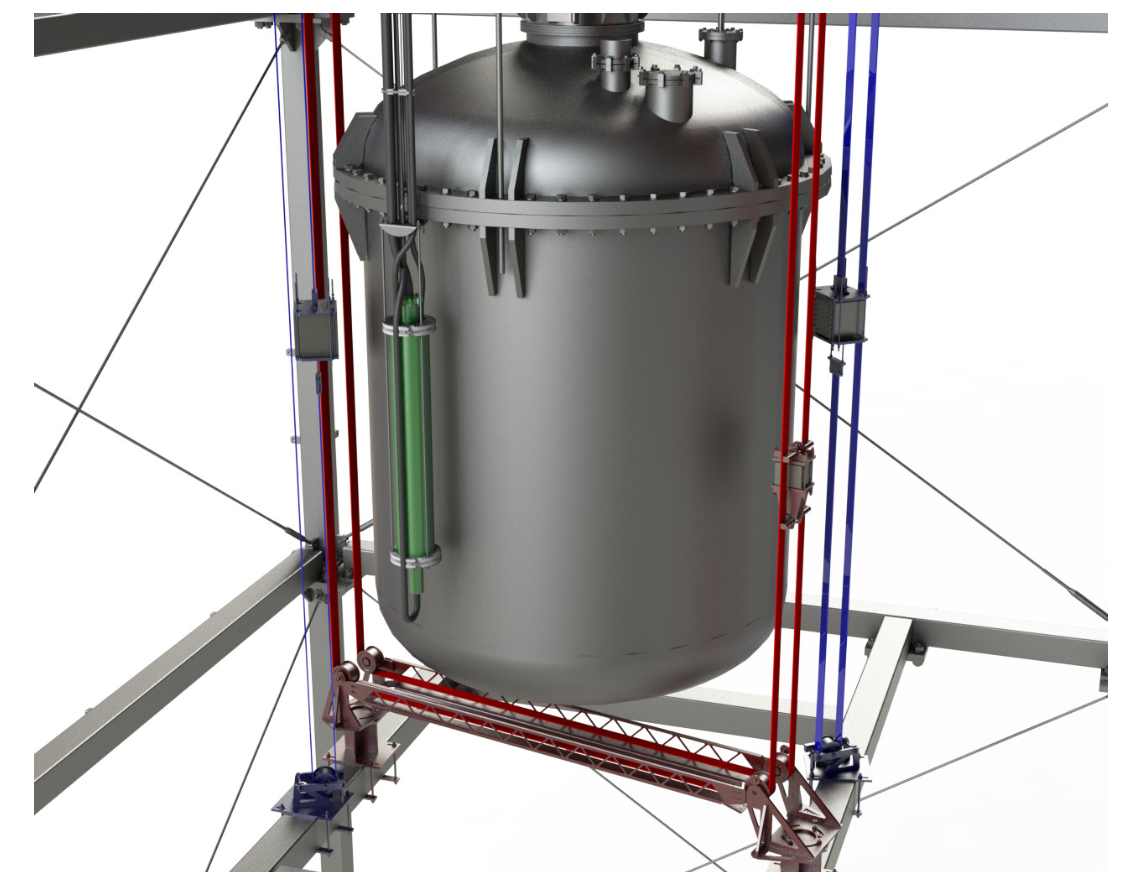
\includegraphics[width=0.8\textwidth]{TPCCalibrations}
\caption{Calibration belts around the cryostat.  The I-belt and U-belt are shown in blue and red and have collimators present.  The green
cylinder is the neutron generator.  Image credit: \citeref{Aprile2017b}.}
\label{fig:xenon1t_calibrations_belts}
\end{figure}

External $\gamma$ sources include \ce{^{137}Cs} with an energy of 661.7 keV, and \ce{^{228}Th} with a number of energies between 511 keV
and 2.614 MeV.  These are stored in W-collimators that restrict the \gammarays to a cone of $40^{\circ}$.  Additionally, the \ce{^{60}Co}
in the materials has 1.173 and 1.333 MeV lines that can also be used.

Nuclear recoil sources \ambe and a deuterium-deuterium (D-D) neutron generator (NG) are also placed in the water tank.  They emit MeV
neutrons (though have different spectrums) and the \ambe is housed in the W-collimator.  Details are discussed in
\secref{subsubsec:er_nr_calibrations_parameter_determ_nr}.



\subsection{Data Acquisition}
\label{subsec:xenon1t_daq}
The data acquisition (DAQ) is in a temperature-controlled room on the second floor of the service building.  It can record the TPC and
muon veto PMTs independently or together.  Signals from the TPC pass through Phillips Scientific 776 amplifiers
where they undergo a 10-fold increase in amplitude.  They, along with the muon veto signals, are then digitized via 100 MHz CAEN V1724
flash analogue to digital converter (ADC) boards (32 in total) that have 40 MHz bandwith, 14 bit resolution, and ranges of 2.25 V and
0.5 V, respectively.  \figref{fig:xenon1t_waveform}
shows a typical waveform recorded by the DAQ.  A single independent clock
connects to each ADC to ensure they are aligned and a 0.1 Hz synchronization signal is passed from a custom-developed GPS-synched
module.

\begin{figure}
\centering
\includegraphics[width=\textwidth]{waveform_xenon1t}
\caption{Example of a waveform from XENON1T.  The bottom panel shows hits (red circles) for each PMT channel with
larger areas representing greater intensity.  An S1 (76.2 PE) is visible at ${\sim}380\ \mathrm{\mu s}$, marked by the blue circle in the
middle panel.  The shape of the S1 (left) and the light seen by the bottom PMT array (center right) are shown in the top panel.  At
${\sim} 1000\ \mathrm{\mu s}$ an S2 (2120.1 PE) occurs.  Its shape (center left) and light distribution in the top PMT array (right) are
shown in the top panel.  The red cross marks the $x \mdash y$ coordinates from the position reconstruction algorithm
(\secref{subsec:det_char_position_reconstruction}).  PMTs near the cross that are white are turned off.  S2s are marked by
green circles in the middle panel.  Two smaller ($< 40\ \mathrm{PE}$) S2s follow the primary S2 by ${\sim}150\ \mathrm{\mu s}$.}
\label{fig:xenon1t_waveform}
\end{figure}

The TPC DAQ reads every pulse $> 0.3\ \mathrm{PE}$ from each PMT independently and regardless of any signal from other
channels.  The read-outs of the ADC boards are passed to six computers at up to $300\ \mathrm{MB\ s^{-1}}$ (${\sim}100\ \mathrm{Hz}$) and
are stored along with relevant information such as time and channel in a MongoDB database.  The sum of the bottom PMTs along with veto
and busy information is constantly read by a separate computer to determine the deadtime.  The DAQ continuously monitors data quality
parameters such as baseline, trigger, and noise.

\begin{figure}
\centering
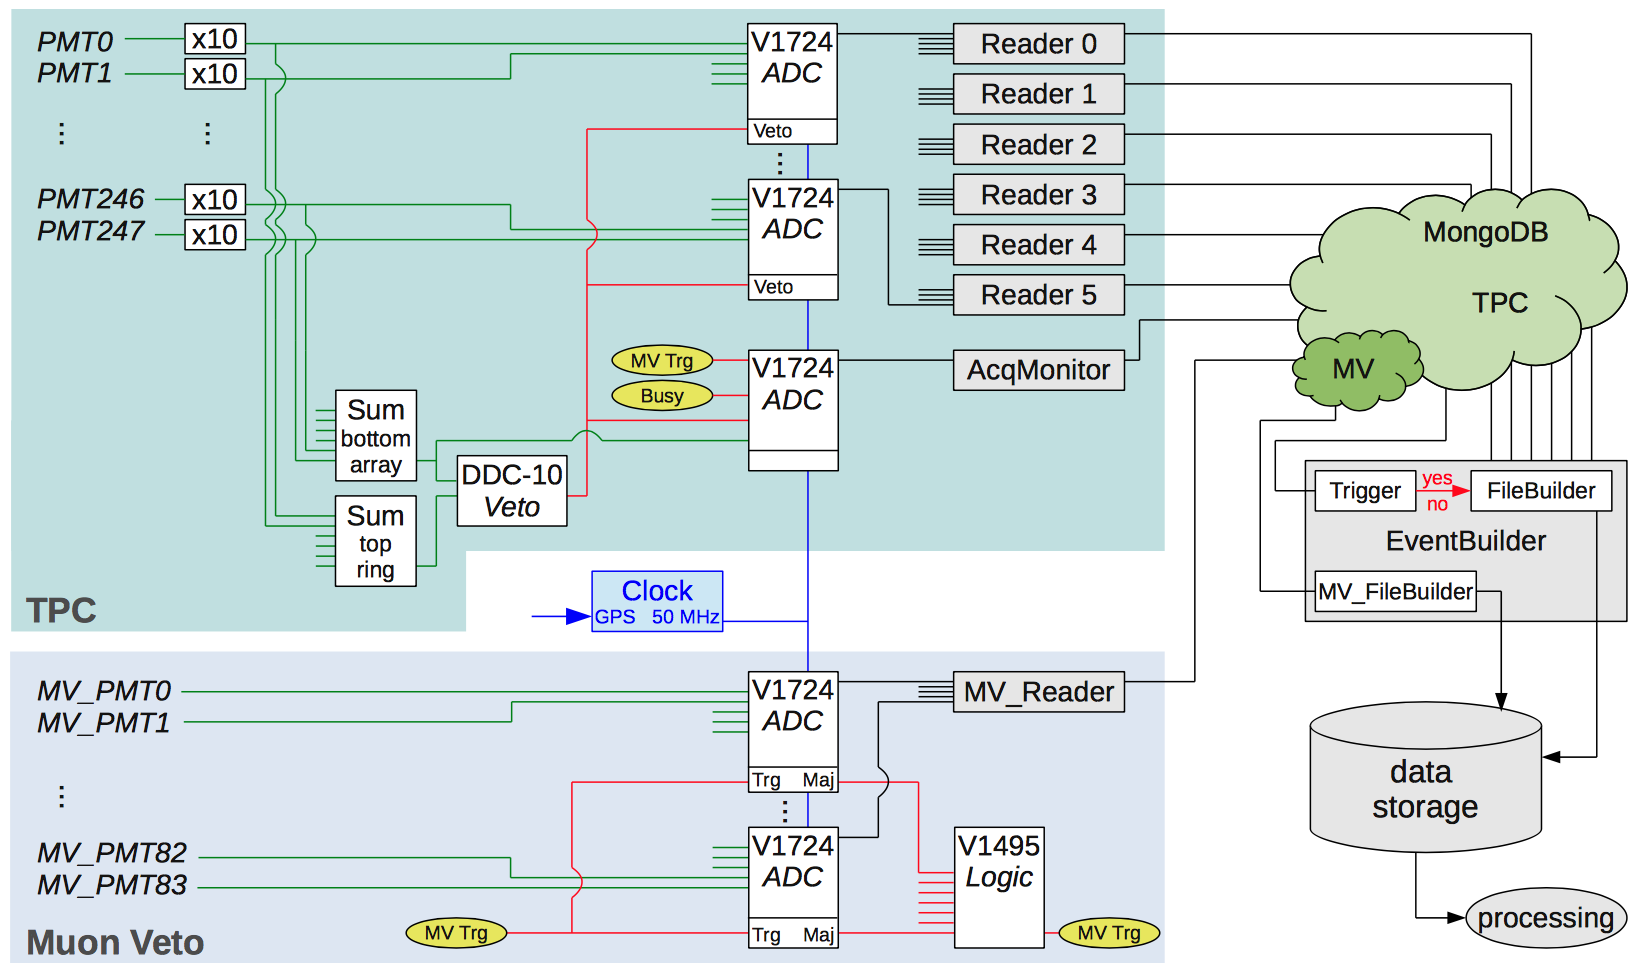
\includegraphics[width=\textwidth]{DAQ}
\caption{Schematic of the data acquisition.}
\label{fig:xenon1t_daq_schematic}
\end{figure}

A software eventbuilder on three server-grade machines decides in real-time if an interaction has occurred by examining the
time-clustering of PMT signals, and opts whether to trigger.  Metadata from the trigger decision is recorded and can be monitored
online to check performance or offline for analysis.  At larger than 200 PE (${\sim}7\ e^-$) the trigger efficiency is $> 99\%$.  The muon
veto uses a simple coincidence trigger that is directed by a CAEN V1495 VME unit.

Two 10 Gbps fibers transfer the raw data to buffer-storage at LNGS for temporary housing.  The raw data is then moved to the US Open
Science Grid and European Grid Infrastructure for processing and backed up in Stockholm.  \figref{fig:xenon1t_daq_schematic} shows an
overview of the DAQ system.

To prevent acquisition of bad data four quality checks are performed - three of which are done in real time during data taking.  The
first is a \textit{high energy veto} that goes to \texttt{TRUE} in the event of a very large S2.  When this occurs the DDC-10 (custom
module) forwards a \texttt{NIM} pulse to the ADC boards, which blocks data from being copied to the readers.  Simultaneously a
\texttt{BUSY ACTIVE} signal is sent from the DDC-10 to the
acquisition monitor digitizer.  After 10 ms the high energy veto returns to \texttt{FALSE}, ending the \texttt{NIM} pulse and resetting
\texttt{BUSY INACTIVE}.  This mode is only used during calibrations.

Aside from the DAQ monitor each of the 32 digitizers feeds a low-voltage differential signaling (LVDS) pulse to the V1495 logic
module.  Each
is \texttt{TRUE} if the memory buffer is nearly full and \texttt{FALSE} otherwise.  This is the \textit{busy veto} and in a
similar fashion to the high energy veto,
the V1495 fans a \texttt{NIM} pulse to the digitizers to block copying of their data to the readers, and sends a \texttt{BUSY TRUE} to the
DAQ monitor digitizer.  The veto is lifted once all digitizers return to less than full memory or 10 ms - whichever is longer.

The final check during data acquisition is the \textit{busy type check}.  It ensures that nowhere in the event was a veto
signal, i.e. the busy signal must set to \texttt{BUSY FALSE}.  This is in part to reject events where a large S2 triggers a high energy
veto that cuts off subsequent smaller S2s (or even part of the large S2) in the same waveform.  It also cuts PMT flashes as they
trigger a busy veto.

The final quality cut is done in processing.  On a small number of occasions events at the end of a dataset some channels
would be missing.  To fix this the final 21 seconds of each run are omitted from analysis.  The 21 seconds comes from the
internal clock of the digitizers, which count from zero to 0x3FFF in 10 ns steps, or roughly 21 seconds.



\subsection{Slow Control System}
\label{subsec:xenon1t_detector_slow_control}
The subsystems are controlled, monitored, and recorded by a slow system.  The system uses General Electric (GE) Programmable
Action Controllers (PACs) and Complicity Supervisory Control And Data Acquisition (SCADA) for hardware and software, respectively.  Nearly
2,500 parameters are stored in a GE Proficy Historian database, which can be queried for analysis offline.  Breach of alarm conditions
(e.g. out of range, connection loss, failure of equipment) triggers notifications via email, pre-recorded voice messages over landline,
and SMS texts to cellular phones.

Individual PACs from the GE RX3i family control sensors and actuators of the purification, cryogenic, krypton distillation,
LXe storage, and water purification systems.  The PACs connect to a private front-end network.  PAC alarms are transmitted using the
GE Alarm\&Event Express tool to the alarm system.  In addition to the SCADA system operations are possible via touch screens.  Open
Platform Communication (OPC) servers, web services, or the Modbus protocol integrate the DAQ, high-voltage supply, and calibration
system motor controllers into the slow control system.  For extra security the system requires certain conditions to be met before
performing potentially unsafe operations.

PACs and OPC servers connect to two redundant SCADA servers on the front-end network.  Two redundant fibers link the experiment to the
aboveground laboratory.  An aboveground building houses supervisory and data storage components including the alarm system, Historian
database, slow control viewer, and primary XENON1T control room.  The slow control system is connected to a backup server outside LNGS
to prevent data loss during a laboratory network failure.  It is powered by an extended on-battery runtime
uninterruptible power supply (UPS) with generator backup.



\section{Detector Characterization}
\label{sec:det_char}
Calibrations are used for detector characterization, monitoring, and measurements of fundamental physics.  In XENON1T
$\mathrm{^{83m}Kr}$, \ce{^{222}Rn}, \ce{^{137}Cs}, \ce{^{228}Th}, americium beryllium (\ce{^{241}AmBe}), a neutron generator, and LEDs
have been used for calibration.
% look at http://www.uni-muenster.de/Physik.KP/AGWeinheimer/Files/theses/Bachelor_Sergej_Schneider.pdf sections 2.2 and 2.3

The most frequent calibration source is $\mathrm{^{83m}Kr}$.  As a noble gas it can be injected directly into the xenon without loss of
purity, and its short half-life and stable decay product mean rates return to normal within a day.  \ce{^{83}Rb}, is installed in the
source box connected to the purification system (\secref{subsec:xenon1t_calibrations_internal}) and decays through electron capture

\begin{equation}
\mathrm{^{83}Rb} + e^- \rightarrow \mathrm{^{83}Kr} + \nu_e
\end{equation}

\noindent with a 74.8\% branching ratio to the metastable state $\mathrm{^{83m}Kr}$.  $\mathrm{^{83m}Kr}$ then de-excites in two steps:
emission of a 32.2 keV
conversion electron with half-life $t_{1/2} = 1.83\ \mathrm{h}$ followed by a second conversion electron at 9.4 keV with
$t_{1/2} = 154.4\ \mathrm{ns}$.  The short interval between the two decays makes tagging events easy and has strong discrimination power
against nominal background.  The events used for studies including detector characterization need to have both S1s resolved
by the DAQ.  To select such events the waveform must have two S1s with a time between them
$\Delta t_{\mathrm{S1}} 500 \mdash 2000\ \mathrm{ns}$.  This
cuts more than 96\% of \metakr events but the high activity is still sufficient to perform high-statistic
analyses.  \figref{fig:calibrations_kr_s1_s2} shows S1 and cS1 for both decays, and \stwob and \cstwob for the 32.2 keV decay for \metakr
events.  While the
$\Delta t_{\mathrm{S1}}$ cut rejects most \metakr events, it is extremely effective at removing background.

\begin{figure}
\centering
\includegraphics[width=\textwidth]{kr_s1_s2_cs1_cs2}
\caption{\metakr 32.2 and 9.4 keV events.  Uncorrected and corrected S1s for both decays are shown in the top left and top right
panels.  The bottom left panel shows S1 and \stwob for the 32.2 keV, and bottom right shows cS1 and $\mathrm{cS2_b}$.}
\label{fig:calibrations_kr_s1_s2}
\end{figure}

The mono-energetic decays are used for a number of
detector characterizations including light collection efficiency (\secref{subsec:det_char_lce}), position reconstruction
(\secref{subsec:det_char_position_reconstruction}), S2 correction maps (\secref{subsec:det_char_s2_position_correction}), and electron
lifetime (\secref{subsec:det_char_elifetime}).


\subsection{PMT Gain}
\label{subsec:det_char_pmt_gain}
The charge per photoelectron that reaches the PMT anode has some inherent spread and varies between phototubes.  Raising the bias
voltage amplifies
the gain and increases sensitivity, while lowering the voltage helps prevent saturation.  Gains also change from variations in
temperature, overexposure to light, count rate, wear, and more.  Phototubes may differ from one another
for all the reasons just mentioned, as well as differences in parts, even microscopic.  Monitoring the single photoelectron (SPE)
response for each PMT is essential for accurately reconstructing the number of photoelectrons from an
event.  This is typically done with an LED inside the TPC.  Blue light is used since LEDs that produce light at relevant wavelengths do
not exist, which despite
being far higher than 178 nm ejects a photoelectron some small fraction of the time.  Each time the LED flashes the PMT signals are
recorded (during normal data taking this requires a pulse larger than some threshold, \secref{subsec:xenon1t_daq}).  After a large
($\mathcal{O}(10^{5})$)
number of trials a histogram is fit to find the SPE gain as shown in \figref{fig:xenon1t_pmt_spe}.  The charge is plotted but the gain is
easily found as $g = \mu_{e} / e$ where $\mu_{e}$ is the mean number of \electron and $e$ is the electron charge.  A large peak is
centered at 0 that corresponds to the baseline noise when no photoelectrons are ejected.  At higher gains a series of
smaller, wider peaks are visible from integer numbers of photoelectrons, starting with 1 at the leftmost.  There is a ``shoulder"
between the baseline and first peak that cannot be explained by only considering signal from integer photoelectrons.  As briefly mentioned
in
\secref{subsec:tpcs_pmts} this comes from photons that pass through the photocathode and hit the first dynode, causing
under-amplified electron avalanche.  This is generally the most challenging aspect to model.

\begin{figure}
\centering
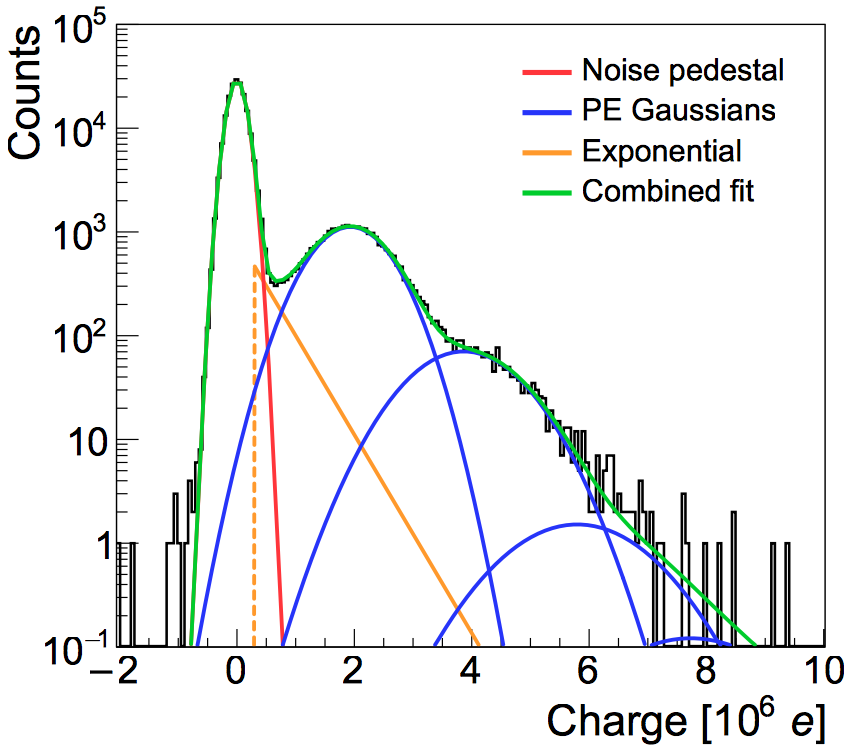
\includegraphics[width=0.6\textwidth]{SPESpectrum}
\caption{Single photoelectron spectrum.}
\label{fig:xenon1t_pmt_spe}
\end{figure}

In \figref{fig:xenon1t_pmt_spe} the spectrum is fit assuming the noise, baseline, and photoelectron peaks are gaussian and the
under-amplification is
an exponential.  The PE gaussians are constrained by $\mu_{N} = N \mu_{e}$ and $\sigma_{N} = \sqrt{N} \sigma_{e}$ where $\sigma_{e}$ is the
standard deviation of the single photoelectron peak and $\mu_{N}$ and $\sigma_{N}$ are the mean and standard deviation for the peak with
$N$ photoelectrons.  Because this simplistic model can add bias recent efforts have gone into alternative methods
of characterization (\citeref{Saldanha2017, 2017Anthony}).  Nonetheless, the combined fit (green) appears to agree will with the data.

The resolution of the PMT is calculated from the SPE spectrum $R = \sigma_{e} / \mu_{e}$.  As the gain grows the resolution should sharpen
until it eventually levels off.  For the R11410-21 models the plateau begins around $2 \mdash 3 \times 10^{6}$ at a resolution of
27\%.  Because the stress on the PMT grows with bias voltage and larger gains create greater saturation it was decided there was no
benefit to exceeding this gain.

\begin{figure}
\centering
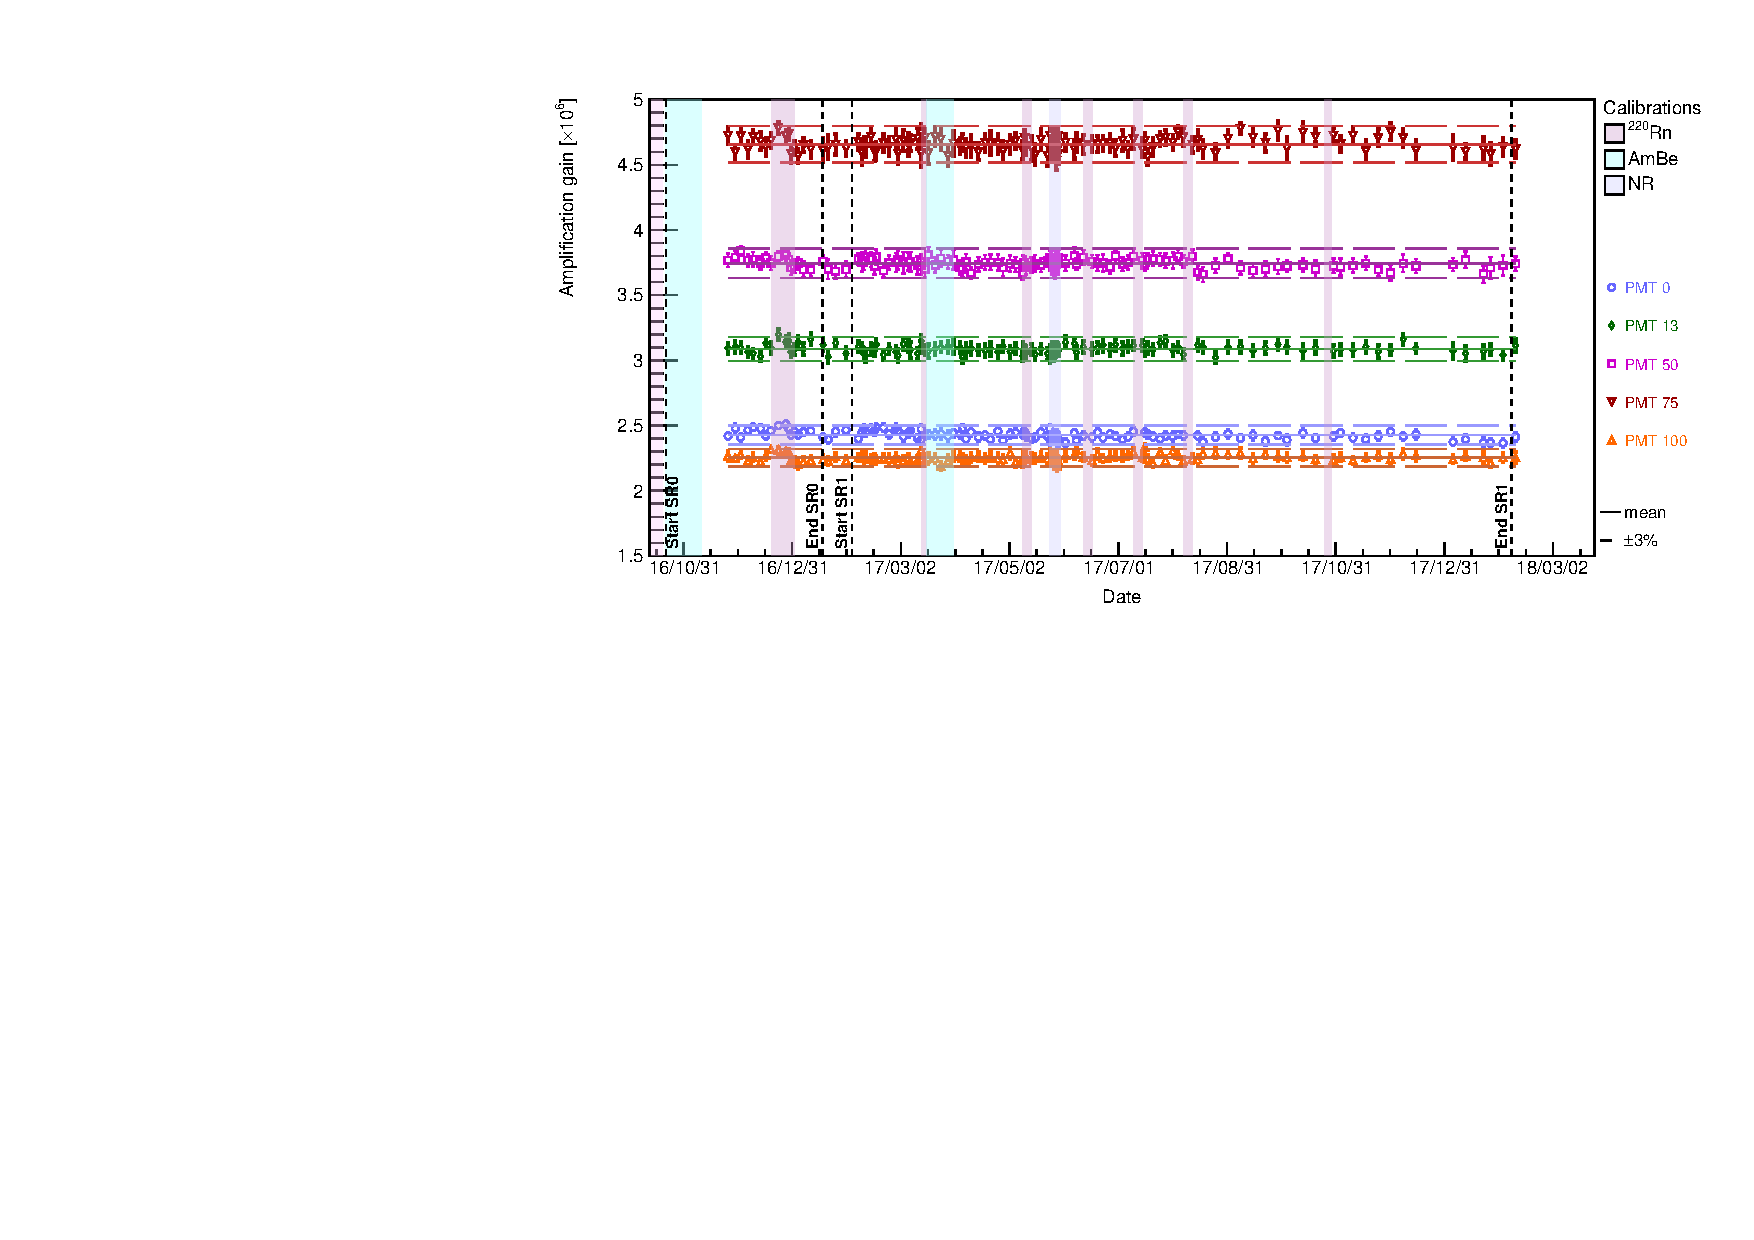
\includegraphics[width=\textwidth]{PMTGainStability}
\caption{Gains for five PMTs monitored for SR0 and SR1.  Means and $\pm 3\%$ are shown.  All appear to be stable.}
\label{fig:xenon1t_pmt_time}
\end{figure}

The relatively poor resolution is apparent in \figref{fig:xenon1t_pmt_spe} as the photoelectron peaks are hard to distinguish.  An
important metric of the SPE spectrum is the peak-to-valley ratio, which divides the first PE peak by the valley that sits between it and
the baseline noise.  Like the resolution it increases for low gains and eventually levels.  For gains of $2 \mdash 3 \times 10^{6}$ the
mean peak-to-valley ratio is ${\sim} 3$.  LED calibrations are regularly performed to identify changes in
gain.  \figref{fig:xenon1t_pmt_time} shows the gain for five PMTs from the beginning of Science Run 0 to the end of Science Run 1.



\subsection{Light Collection Efficiency}
\label{subsec:det_char_lce}
The light observed by a PMT depends in part on the position of the event.  The light collection efficiency (LCE),
$\mathcal{C}_{\mathrm{lce}}(x, y, z)$ - seen in \figref{fig:calibrations_lce_polar} - quantifies these differences.  Position-dependent
variations exist because the location of
the interaction dictates effects due to detector features and physics.  First, the the solid angle encompassing the PMT arrays
for an event is not uniform
throughout the detector.  It is greatest near the top or bottom of the TPC and at small radii.  The measured intensity of the
scintillation
from the S1 depends on the fraction of photons that reach PMTs and how far the light must travel.  Interactions near the
wall have a lower observed intensity because of this.  The quantum efficiency (QE) of the PMTs (\figref{fig:xenon1t_pmt_array}) is also a
factor, since those with larger values are more likely to produce a photoelectron.  Because the PMTs with the highest QE were placed in
the
center of the bottom array (\secref{subsec:xenon1t_pmts}) events that happen around that region have a higher likelihood of detection,
while those in the top corners have the lowest.

Because PTFE has a small but $> 0$ absorption the intensity of the scintillation decreases with each reflection.  Therefore light
that is emitted in the $\hat{r}$-direction can be severely dampened.  Photon loss is amplified by the absorption of light by
impurities in the LXe as well, so longer traversed distances lead to fewer photons (\secref{subsec:importance_procedure_effects_photons}).

The index of refraction of LXe ${\sim} 1.7$
gives a critical angle of $\theta_c = 36^{\circ}$.  The light that reaches the top PMTs for an event at
$z = -10\ \mathrm{cm}$ is restricted to a radius of just 13.6 cm at the liquid surface (the total solid angle if also at
$r = 0\ \mathrm{cm}$ is $83.9^{\circ}$).  While the light will be internally reflected towards the bottom array, it will
be diminished by reflections from the PTFE and extended travel distances. In comparison, light
directed towards the surface from an event 10 cm above the cathode ($r = 0$)
has $\theta < \theta_c$ everywhere.  Some scintillation that reflects off the PTFE on the way up will rebound off the surface, but its
contribution is small in comparison.

\begin{figure}
\centering
\includegraphics[width=\textwidth]{lce_map_polar}
\caption{Light yield in slices of $z$ and $\phi$ from \metakr 32.2 keV decay.}
\label{fig:calibrations_lce_polar}
\end{figure}

Calibrating the LCE requires a mono-energetic peak - preferably one near our DM energy range.  For this we use the light from the
$\mathrm{^{83m}Kr}$ 32.2 keV conversion electron.  While more than twice the DM energy range, a lower-energy option does
not exist.  \figref{fig:calibrations_lce_polar} shows the LCE binned in $r$, $\phi$, and $z$.  It changes by roughly a factor of 2 between
the top and bottom.  Unpowered PMTs are responsible for the sudden changes in the bottom of the TPC between adjacent $r$ and $\phi$ bins.

Changing the electric field will cause recombination for electronic recoils of different energies to change by different amounts.  The
same is true for an electronic and nuclear recoil of the same energy.  Therefore the LCE map in \figref{fig:calibrations_lce_polar} is
technically correct only for a 32.2 keV electronic recoil.  However, because the TPC was designed for a uniform electric field - and
simulations confirm this, especially for events more than a few cm away from the wall - differences in
$\mathcal{C}_{\mathrm{lce}}(x, y, z)$ can be ignored.



\subsection{Position Reconstruction}
\label{subsec:det_char_position_reconstruction}
TPCs allow 3-dimensional position reconstruction.  Since the drift velocity $v_d$
is constant in LXe the depth is $z = -v_d t_d$ where $t_d$ is the drift time ($z$ is defined to be negative with
$z = 0$ at gate).  The drift fields for SR0 and SR1 were $E_d = 118.6\ \mathrm{V\ cm^{-1}}$ and $81.3\ \mathrm{V\ cm^{-1}}$,
respectively, with $2.2\ \mathrm{V\ cm^{-1}}$ RMS variations.  The fields correspond to drift velocities of
$v_d = 1.440\ \mathrm{mm\ \mu s^{-1}}$ and $1.332\ \mathrm{mm\ \mu s^{-1}}$ and
maximum drift times of $t_{d, \mathrm{max}} = 672.8\ \mathrm{\mu s}$ and $727.3\ \mathrm{\mu s}$ (TPC drift length is 96.9
cm at$-100^{\circ}\mathrm{C}$).

\begin{figure}
\centering
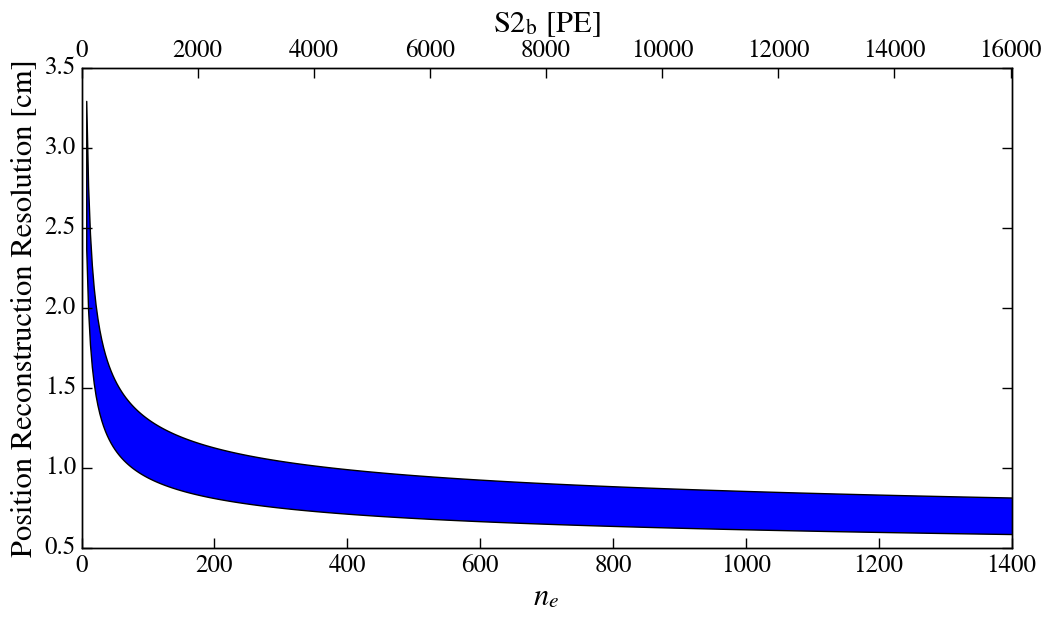
\includegraphics[width=\textwidth]{PosRecRes}
\caption{$x \mdash y$ position reconstruction resolution $\pm 1\sigma$ for SR1 as a function of number of electrons and
$\mathrm{S2_b}$.  At lower $n_e$ the
resolution becomes worse due to the limited S2 scintillation.  At low-energies ($n_e \lesssim 100\ e^-$,
$\mathrm{S2_b} \lesssim 1000\ \mathrm{PE}$) the position resolution becomes extremely poor.}
\label{fig:calibrations_position_reconstruction_res}
\end{figure}

The $x \mdash y$ coordinates are found by using the intensity of light from the S2 observed by each PMT in the top array (also
known as PMT hit pattern).  For XENON1T two reconstruction algorithms were mainly used to convert the PMT hit pattern to $x$ and $y$.  The
first was a neural net (NN) using the Fast Artificial
Neural Network (FANN) library with 24 and 29 nodes in the two hidden layers (sequentially).  The second matches the real with expected hit
patterns after weighting four separate algorithms for its seed, and is known as top pattern fit (TPF).  Both algorithms were trained using
Monte Carlo and optimized with $\mathrm{^{83m}Kr}$ data, and achieved a position resolution of $\lesssim 2\ \mathrm{cm}$.  For the
combined-run analysis the NN was used because the TPF algorithm was more sensitive to dead PMTs and showed some artificial discontinuity
in the $\hat{r}$-direction.  The position reconstruction resolution for the NN is shown in
\figref{fig:calibrations_position_reconstruction_res}.  \figref{fig:calibrations_position_reconstruction} shows the position distribution
of events in SR1 along with
the 1 ton fiducial mass that was used in originally used in the SR0-only results (\citeref{Aprile2017f}), the 1.3 t used in the new
analysis, and the active volume.

\begin{figure}
\centering
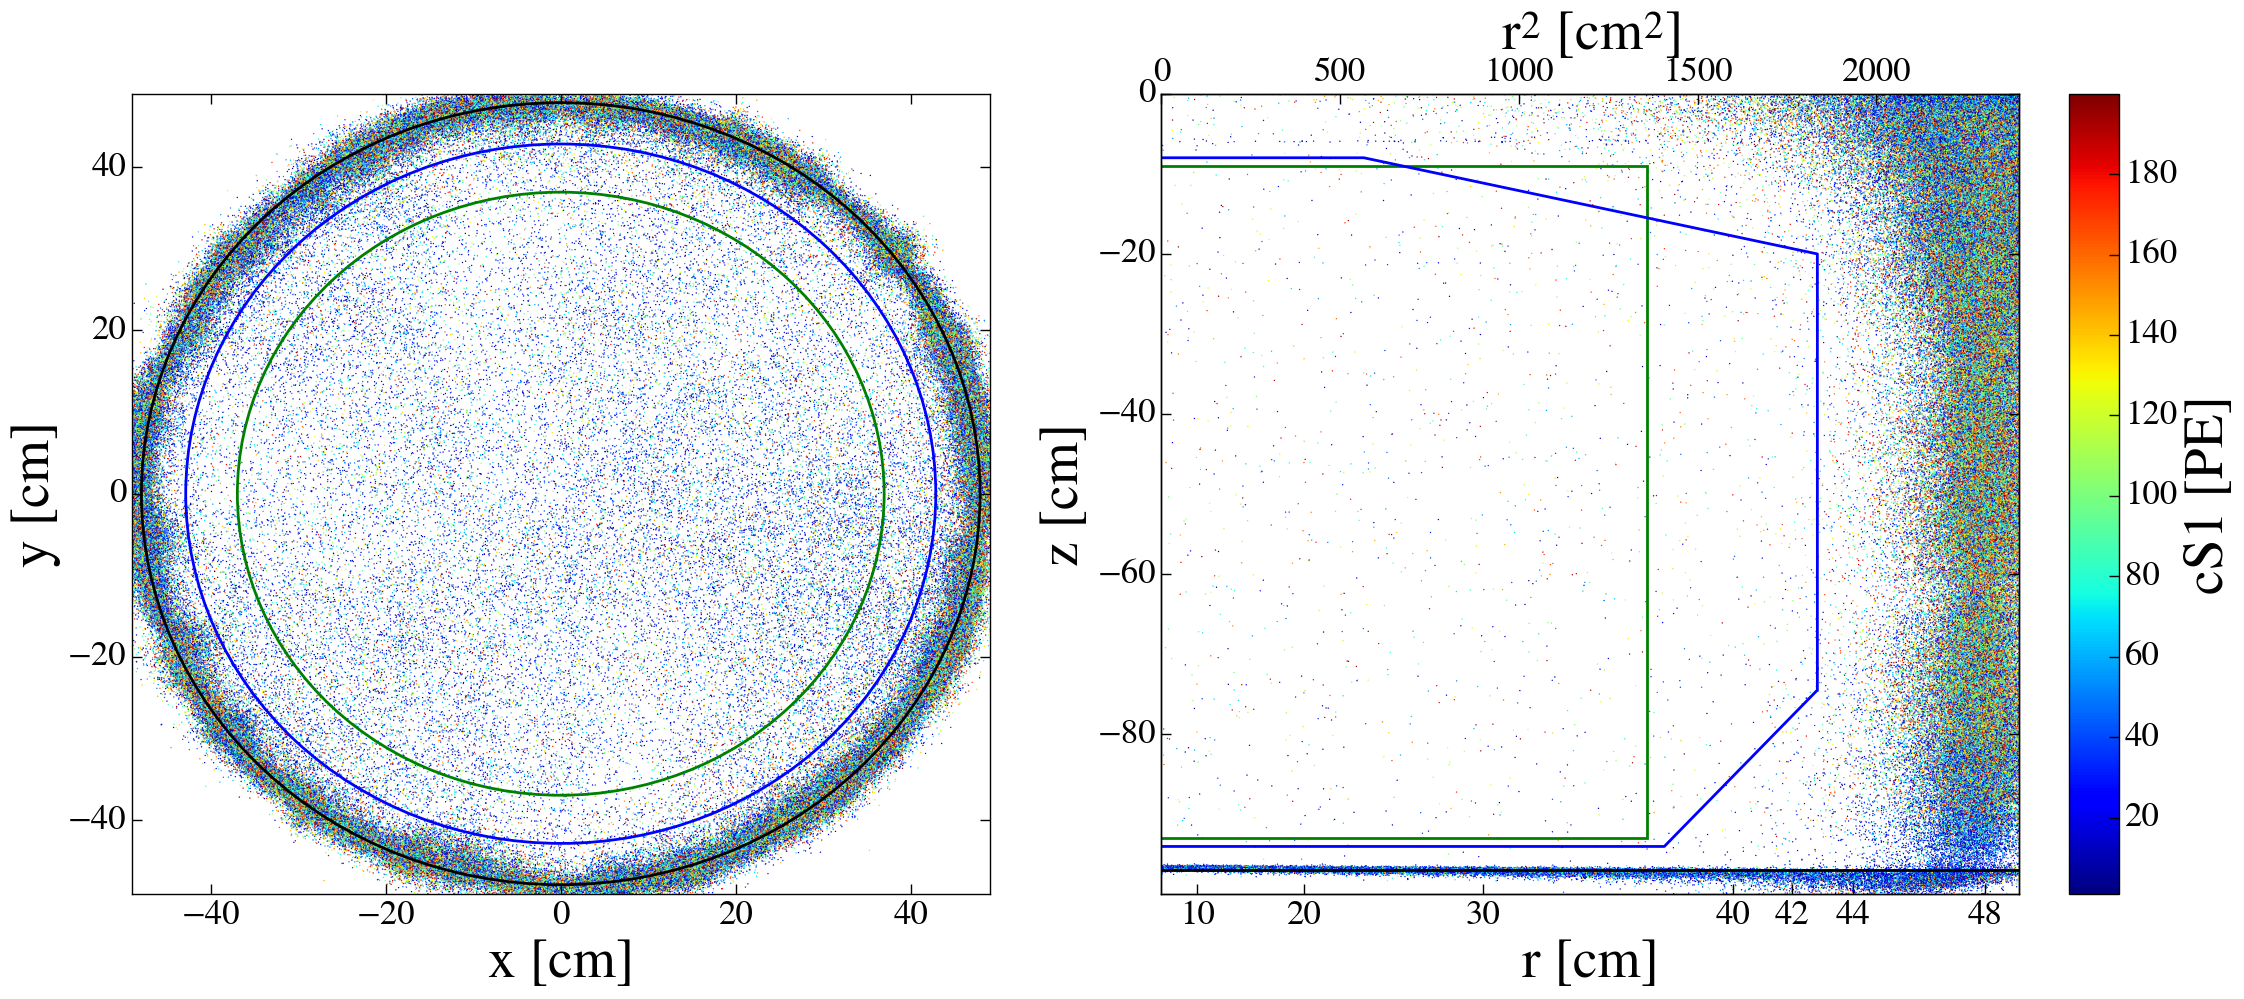
\includegraphics[width=\textwidth]{FVBoth}
\caption{Positions of background events for SR1.  The 1 ton fiducial mass used in the SR0-only analysis is defined by
$-92.9 < z < -9\ \mathrm{cm}$, $r < 36.94\ \mathrm{cm}$ and shown in green.  The 1.3 ton fiducial mass for this analysis has a more
complicated shape, having $z_\mathrm{min} = -94\ \mathrm{cm}$,
$z_{\mathrm{max}} = -8\ \mathrm{cm}$, and $r_{\mathrm{max}} = 42.84\ \mathrm{cm}$.  It is outlined in blue ($r_{\mathrm{max}}$ is shown
in left panel).  The active volume is marked in black.  Events that appear outside the active volume are wall events that were not
properly
reconstructed.  Those that appear below the cathode result extended drift times due to field inhomogeneities, which is why they
become more exaggerated near the bottom corner of the TPC.}
\label{fig:calibrations_position_reconstruction}
\end{figure}



\subsection{S2 $\mathbf{x \mdash y}$ Correction}
\label{subsec:det_char_s2_position_correction}
The S2 scintillation observed by PMTs depends on its $x \mdash y$ coordinates (the $z$-correction is calculated using the electron
lifetime in \secref{subsec:det_char_elifetime}).  Most of the light seen by the top array is focused on a small group of PMTs directly
over the extraction site, while a large
solid angle causes a more uniform spread on the bottom array.

The top and bottom correction maps are shown in \figref{fig:calibrations_s2_maps}.  The relative S2 light yield is shown, which can be
thought of as variations in $g_2$ or the single electron gain $G_e$ (\secref{subsec:det_char_single_electron_gain}).  The local
fluctuations are primarily the result
of unpowered PMTs.  The steeper local variations in the top array result from the light being more concentrated.  At larger radii the
S2s are higher due to a small sagging of the anode.  The increase in the bottom array as $r \rightarrow 0$ is 
mainly due to the higher QE.  The large solid angle creates a roughly homogeneous azimuthal distribution.

\begin{figure}
\centering
\includegraphics[width=\textwidth]{s2_relative_light_yield}
\caption{Relative S2 light yield for the top (left) and bottom (right) PMT arrays.  Light from \electron extracted across the GXe is
concentrated in the small number of PMTs directly above in the top array.  Large fluctuations in the top array are due primarily to dead
PMTs while
smaller are from variation in gains.  A larger solid angle results in a more uniform distribution across $\phi$ in the bottom array.}
\label{fig:calibrations_s2_maps}
\end{figure}

Because the position must be reconstructed (\secref{subsec:det_char_position_reconstruction}) before any correction can be
applied, events that have poor position resolution (mainly either below dead PMTs or low-energy) are more likely to have a greater
deviation from true values.



\subsection{Electron Lifetime}
\label{subsec:det_char_elifetime}
The electron lifetime $\tau_{e}$ (see \secref{subsec:tpcs_working_principle} for impurity attachment details) measures the charge $q$
that is lost as electrons drift to the liquid-gas interface.  It is given by

\begin{equation}
q(t_d) = q_0 e^{-t_d / \tau_{e}}
\label{eq:det_char_elifetime}
\end{equation}

\noindent where $q_0$ is the initial charge that escapes recombination.  Generally when calculating $\tau_{e}$ a mono-energetic source is
used so that $q_0$ is the same throughout the detector and the collected charge is only dependent on $t_d$.  During dark matter data
taking the electron lifetime is monitored via background
\ce{^{222}Rn} and \ce{^{218}Po} $\alpha$-decays.  Because materials with low \ce{^{222}Rn}
emanation were chosen, electron lifetime measurements usually require 24-48 hours of data.  Alternatively, calibrations
have significantly higher (${\sim}50\ \mathrm{Hz}$) statistics, allowing measurements with much better precision.

The 32.2 keV $\mathrm{^{83m}Kr}$ de-excitation is an effective method to measure $\tau_{e}$.  The number of events
from a typical calibration of 2-3 days is in the millions, so even with $< 4\%$ acceptance after the $\Delta t_{\mathrm{S1}}$ cut the
number of usable events
is ${\sim}10^5$ with effectively no background.  \figref{fig:det_char_elifetime_kr} shows an example of an electron lifetime calculation
using $\mathrm{^{83m}Kr}$.

\begin{figure}
\centering
\includegraphics[width=\textwidth]{kr_electron_lifetime_linear}
\caption{Electron lifetime measurement using $\mathrm{^{83m}Kr}$.  The red line represents the best-fit value of
$671.18 \pm 4.14\ \mathrm{\mu s}$ and extends over the region the fit was computed.  Details on the method of the fit are in
\secref{subsec:electron_lifetimes_measurement_kr}.}
\label{fig:det_char_elifetime_kr}
\end{figure}

Another high-statistic measurement is possible during \ce{^{220}Rn} calibrations.  Primarily used for the 569.9 keV $\beta$-emission of
its decay chain progeny \ce{^{212}Pb} (\secref{subsubsec:er_nr_calibrations_parameter_determ_er}), a number of elements along the chain
undergo $\alpha$-decays and can be used to measure $\tau_e$.  \tabref{tab:alpha_decays} lists the main $\alpha$-emitters in both the
\ce{^{222}Rn} and \ce{^{220}Rn} chains.  Because \ce{^{220}Rn} calibration
data is only used after the source valve is closed, \ce{^{220}Rn} and \ce{^{216}Po} won't be present due to their short half-lifes of
55.6 s and 145 ms.  However \ce{^{212}Bi} emits a 6.207 MeV $\alpha$ as it decays to \ce{^{208}Tl} with a
branching ratio of 36.9\%.  A typical electron lifetime using \ce{^{212}Bi} is shown in the right panel of
\figref{fig:calibrations_elifetime}.

In past experiments external \gammaray sources were an effective tool for measuring $\tau_e$.  The ease of placing a source near the
detector for calibration and removing when finished meant background data could resume immediately.  One of the most common sources has
been \ce{^{137}Cs}, whose decay

\begin{equation}
\mathrm{^{137}Cs} \rightarrow \mathrm{^{137}Ba} + e^- + \overline{\nu}_e
\end{equation}

\noindent leaves barium in metastable state.  As $\mathrm{^{137m}Ba}$ de-excites it emits a 661.7 keV $\gamma$-ray, whose mean
free path of ${\sim}5\ \mathrm{cm}$ allowed it to reach the fiducial volumes.  For
XENON1T and other ton-scale detectors to come it is less effective, as an attempt shortly after the detector came online showed.  Using
\ce{^{137}Cs} a Compton spectrum and total absorption peak were visible but only in the region closest to the source and after many hours
of data.  The 163.9 and 236.2 keV de-excitations of $\mathrm{^{131m}Xe}$ and $\mathrm{^{129m}Xe}$ following a nuclear
recoil calibration are effective because they uniformly distribute throughout the xenon.  However, following the \ambe and neutron
generator calibrations their activity was on the order of \ce{^{222}Rn}, and as they de-excited larger time windows were required for
a fit.

\bgroup
\def\arraystretch{1.2}
\begin{table}
\centering
\begin{tabular}{cccccc}
\hline
\hline
Isotope & Daughter & Energy & $t_{1/2}$ & Chain \\
\hline
\ce{^{222}Rn} & \ce{^{218}Po} & 5.590 MeV & 3.82 d & \ce{^{222}Rn} \\
\ce{^{218}Po} & \ce{^{214}Pb} & 6.115 MeV & 3.10 m & \ce{^{222}Rn} \\
\ce{^{214}Po} & \ce{^{210}Pb} & 7.833 MeV & $164.3\ \mathrm{\mu s}$ & \ce{^{222}Rn} \\
\ce{^{210}Po} & \ce{^{206}Pb} & 5.407 MeV & 138.4 d & \ce{^{222}Rn} \\
\ce{^{220}Rn} & \ce{^{216}Po} & 6.405 MeV & 55.6 s & \ce{^{220}Rn} \\
\ce{^{216}Po} & \ce{^{212}Pb} & 6.906 MeV & 145 ms & \ce{^{220}Rn} & \\
\ce{^{212}Bi} & \ce{^{208}Tl} & 6.207 MeV & 1.01 d & \ce{^{220}Rn} & \\
\ce{^{212}Po} & \ce{^{208}Pb} & 8.954 MeV & 299 ns & \ce{^{220}Rn} & \\
\hline
\hline
\end{tabular}
\caption{$\alpha$-decays with high branching ratios for \ce{^{222}Rn} and \ce{^{220}Rn} decay chains.  \ce{^{222}Rn} emanates from
detector materials and makes up part of our
background so it and \ce{^{218}Po} are used to continually monitor $\tau_{e}$.  \ce{^{220}Rn} is used for electronic recoil calibrations,
so a high-statistic measurement with \ce{^{212}Bi} is possible.  Those with $< 0.1\%$ branching ratio
(\ce{^{218}At}, \ce{^{218}Rn}, \ce{^{214}Bi}, \ce{^{210}Pb}, \ce{^{210}Bi}, \ce{^{209}Bi} for \ce{^{222}Rn} chain, \ce{^{220}Ra} and
\ce{^{216}Rn} for \ce{^{220}Rn} chain) are not listed.}
\label{tab:alpha_decays}
\end{table}
\egroup

\begin{figure}
\centering
\includegraphics[width=\textwidth]{electron_lifetime_evolution_sr0_sr1}
\caption{Electron lifetime over SR0 and SR1.  Markers represent measurements using the 32.2 keV decay of
$^{83\mathrm{m}}\mathrm{Kr}$.  The green line and shaded region represent the median and credible region using the posterior of the
fit.  A hotspot in June forced a gate washing, where the
gate was briefly lifted out of the LXe.  It is suspected the LXe came in contact with parts of the TPC previously only in gas, injecting
impurities into the liquid.  The model is derived using \alphadecays from \ce{^{222}Rn}, \ce{^{220}Rn}, and \ce{^{218}Po} and is
discussed in \secref{sec:electron_lifetime_model}.}
\label{fig:det_char_elifetime_evolution}
\end{figure}

The electron lifetimes from $\alpha$-decays was observed to be smaller than $\beta$s or $\gamma$s.  While energies of \alphadecays are
significantly higher the charge yield is extremely low (\figref{fig:tpcs_signals_drift_field}).  Because the dark matter region of
interest is low-energy and unaffected by $\alpha$ interactions the electron lifetime derived from $\mathrm{^{83m}Kr}$ was used for this
analysis.  The
electron lifetime used for Science Runs 0 and 1 is shown in \figref{fig:det_char_elifetime_evolution}.  The flattening in $\tau_{e}$
around November 2017 may be indicative of a small leak as mentioned in \secref{subsubsec:backgrounds_electronic_krypton}.  Details on the
electron lifetime model are discussed in \secref{sec:electron_lifetime_model}.



\subsection{Secondary Scintillation Gain}
\label{subsec:det_char_single_electron_gain}
While S2s are measured in photoelectrons, an important parameter of
interest is the number of \electron that were extracted across the GXe.  To convert between the two we need to measure the number of
detected photons per $e^-$, also known as the \textit{secondary scintillation gain}, or \textit{single electron gain} $G_e$.  To do so we
look at the
smallest features in the waveforms of events that have the width of an S2, and therefore may be a low integer of $e^-$.  These can
result
from photoionization of detector metals such as the gate or cathode, photoionization of impurities in the LXe, and delayed extraction
of \electron from the surface.

The number of photons emitted depends on - among other things - the electric field between the anode and gate $E_g$.  Details of the
relation can be found in \secref{subsec:tpcs_working_principle} and \eqnref{eq:electronlum}.  The sagging - although small - of the
anode changes $E_g$ slightly along $r$ as mentioned in \secref{subsec:det_char_s2_position_correction} and shown in
\figref{fig:calibrations_s2_maps} (top).  Additionally the dielectric constant of LXe and GXe are different, so a change in liquid level
causes an inhomogeneous shift in field, so levelmeters continually monitor it.

Poisson processes give a good approximation to both $G_e$ and the number of photons detected by the PMTs.  Effects like variation in $E_g$
and PMT detection efficiencies produce smearing.  The single electron spectrum can be modeled as

\begin{equation}
\frac{1}{1 + e^{-(x - A) / B}}\ \sum_{k = 1} h_k\ \mathrm{exp} \bigg( -\frac{(x - k \mu_1)^2}{2 k \sigma_1^2} \bigg)
\label{eq:det_char_single_electron_gain_model}
\end{equation}

\noindent where here $x = \mathrm{S2}$.  Each term in the sum refers to a peak composed of $k$ electrons with amplitude $h_k$.  The
peaks are assumed gaussian with constraints $\mu_k = k \mu_1$ and $\sigma_k^2 = k \sigma_1^2$.  A Fermi-Dirac is used to model the
efficiency of the S2 peak finder algorithm.

Single electrons can be easily found by looking after the primary S2, where photoionization may liberate some small number of $e^-$.  An
example of a single electron spectrum is shown in \figref{fig:calibrations_single_electron_gain_num_photons} where S2s that occurred
between $60 \mdash 727.3\ \mathrm{\mu s}$ after the primary S2.  The lower bound of $60\ \mathrm{\mu s}$ is chosen to
ensure the single electrons are from photoionization, while the upper bound is set to the maximum drift time since the longest
between the primary and single electron S2s should be from photoionization of the cathode.  The best-fit values from
\eqnref{eq:det_char_single_electron_gain_model} are given in \tabref{tab:det_char_single_electron_gain_vals}.

\begin{figure}
\centering
\includegraphics[width=\textwidth]{SEspectrum}
\caption{Single electron spectrum.  Peaks correspond to integer numbers of \electron and are visible and the spectrum is fit
with \eqnref{eq:det_char_single_electron_gain_model} (blue).  Individual peaks for for $1 e^-$ (magenta), $2 e^-$ (green), $3 e^-$ (red),
$4 e^-$ (light purple), $5 e^-$ (brown), and $6 e^-$ (dark blue), along with the processor efficiency (red) are drawn.  Best-fit values
are listed in \tabref{tab:det_char_single_electron_gain_vals}.}
\label{fig:calibrations_single_electron_gain_num_photons}
\end{figure}

\begin{table}
\centering
\begin{tabular}{ccccc}
\hline
\hline
Variable & Best-fit value & Units & $f$ \\
\hline
$A$ & $11.02 \pm .27$ & PE & $-$ \\
$B$ & $5.52 \pm 0.20$ & PE & $-$ \\
$\mu_1$ & $26.71 \pm 0.05$ & PE & $-$ \\
$\sigma_1$ & $7.64 \pm 0.02$ & PE & $-$ \\
$h_1$ & $(4.62 \pm 0.04) \times 10^4$ & $-$ & 0.691 \\
$h_2$ & $(1.024 \pm 0.005) \times 10^4$ & $-$ & 0.153 \\
$h_3$ & $4726 \pm 29$ & $-$ & 0.071 \\
$h_4$ & $2242 \pm 27$ & $-$ & 0.041 \\
$h_5$ & $1583 \pm 36$ & $-$ & 0.024 \\
$h_6$ & $1330 \pm 55$ & $-$ & 0.020 \\
\hline
\hline
\end{tabular}
\caption{Best-fit values of \figref{fig:calibrations_single_electron_gain_num_photons} using
\eqnref{eq:det_char_single_electron_gain_model} with $1 \mdash 6 e^-$.  The fraction of total events $f$ for the $k^{\mathrm{th}}$ peak is
defined as $h_k / \sum_{k = 1}^{6} h_k$ using the best-fit parameters.}
\label{tab:det_char_single_electron_gain_vals}
\end{table}



\subsection{Average Photon Detection and Charge Extraction Efficiencies}
\label{subsec:det_char_photon_charge_efficiencies}
Applying the above corrections converts $\mathrm{S1} \rightarrow \mathrm{cS1}$ and $\mathrm{S2} \rightarrow \mathrm{cS2}$ where cS1 and
cS2 are the corrected S1 and S2.  An event of the same energy and type at the same electric field will result in cS1s and
cS2s that only differ due to physical fluctuations.  For XENON1T the top PMT array for S2s is ignored.  To differentiate from the total S2,
\stwob and \cstwob are used to represent the portion
of the S2 and cS2 observed by the bottom array.  Everything that follows in this chapter uses \stwob and $\mathrm{cS2_b}$.

\begin{figure}
%    \centering
    \begin{subfigure}[t]{0.4\textwidth}
%        \centering
        \includegraphics[height=4cm]{g1_g2_chisquare_pax_v680_hax_v240_feb17tofeb18_from_christian_other}
    \end{subfigure}%
    \begin{subfigure}[t]{0.65\textwidth}
%        \centering
        \includegraphics[height=4cm]{g1_g2_time_evolution}
    \end{subfigure}
    \caption{(left) Example of fitting cS1 and \cstwob from mono-energetic signals to find $g_1$ and g$_{2\mathrm{b}}$.  (right) Evolution
    of $g_1$ and g$_{2\mathrm{b}}$ over the first eight months of SR1.  They are stable to within 0.4\% and 1.4\% ($\pm 1 \sigma$ credible
    intervals) respectively.}
	\label{fig:calibrations_photon_charge_efficiences_g1_g2}
\end{figure}

The processes
for light and charge production were described in \secref{sec:scintillation}.  For electronic recoils atomic motion is
not a factor so all of the energy produces a number of quanta $n_q = E_{er} / W$ where $E_{er}$ is the ER energy and
$W = 13.7 \pm 0.2\ \mathrm{eV}$ is the average energy to create an exciton or electron-ion pair.  The number of quanta can be broken
down as

\begin{equation}
n_q = n_{\gamma} + n_e
\end{equation}

\noindent where $n_{\gamma}$ are $n_e$ are the number of photons and \electron produced, respectively.  This can be rewritten in terms of
observables as

\begin{equation}
\frac{E_{er}}{W} = \frac{\mathrm{cS1}}{g_1} + \frac{\mathrm{cS2_b}}{\eta G_e}
\label{eq:calibrations_s1_s2}
\end{equation}

\noindent where $n_{\gamma} = \mathrm{cS1} / g_1$ and $n_e = \mathrm{cS2_b} / \eta G_e$ (here we now take $G_e$ to be the single electron
gain as measured by the bottom PMT array) where $g_1$ is the average light collection
efficiency and $\eta$
is the \textit{extraction efficiency} - that is, the probability of extracting an \electron from the liquid into the gas.  The average
gain for an \electron then that escapes recombination is $g_{2 \mathrm{b}} = \eta G_e$.  \eqnref{eq:calibrations_s1_s2} has two unknowns:
$g_1$ and $\eta$ (or $g_{2 \mathrm{b}}$).  Rearranging gives

\begin{equation}
\frac{\mathrm{cS2_b}}{E_{er}} = \frac{g_{2\mathrm{b}}}{g_1} \frac{\mathrm{cS1}}{E_{er}} - \frac{g_{2 \mathrm{b}}}{W}
\end{equation}

\noindent and shows $g_1$ and $g_{2\mathrm{b}}$ can be found by using a linear fit if more than one energy is
used.  \figref{fig:calibrations_photon_charge_efficiences_g1_g2} (left) presents this for several lines
during SR1, giving
$g_1 = 0.1426 \pm 0.0001_{\mathrm{stat}} \pm 0.0017_{\mathrm{sys}}\ \mathrm{PE/ph}$ and
$g_{2 \mathrm{b}} = 11.55 \pm 0.01_{\mathrm{stat}} \pm 0.24_{\mathrm{sys}}\ \mathrm{PE/e^-}$ ($\eta = 0.933$).  Because $g_1$ depends on
the PMTs, $\eta$ on the anode-gate electric field, and $G_e$ on $E_g$, pressure, and distance between the gate and anode they are
independent of the
drift field.  $g_1$ and $g_{2 \mathrm{b}}$ were monitored over the
course of SR0 + SR1.  \figref{fig:calibrations_photon_charge_efficiences_g1_g2} (right) shows both
were stable to $< 1.5 \%$.



\subsection{Combined Energy Spectrum}
\label{subsec:det_char_ces}
After solving for $g_1/\eta/g_{2 \mathrm{b}}$ in \eqnref{eq:calibrations_s1_s2} $E$ can be reconstructed for electronic recoil
events.  The XENON1T
background combined energy spectrum is shown in \figref{fig:calibrations_photon_charge_efficiences_ces} for the 1 t fiducial volume during
SR1.  Peaks are labeled with their respective energy and responsible
isotope.  \figref{fig:calibrations_photon_charge_efficiences_ces} shows during DM data taking some $\mathrm{^{83m}Kr}$ is present, most
likely from \ce{^{83}Rb} that was absorbed in the getters and later decayed ($t_{1/2} = 86.2\ \mathrm{days}$).  $\mathrm{^{129m}Xe}$ and
$\mathrm{^{131m}Xe}$ are also visible though the majority of their de-excitations occur in the weeks following the \ambe and the NG
calibrations.  Other visible lines are listed in \tabref{tab:calibrations_photon_charge_efficiences_ces_resolution}.

High energy \gammarays can Compton scatter a number of times before photoelectric absorption (\figref{fig:phot_atten}) or leaving the
detector.  This, along with the $2 \nu \beta \beta$-decay of \ce{^{136}Xe} and \betadecays of isotopes such as \ce{^{214}Pb} create the
underlying irregular background.

\bgroup
\begin{table}
\centering
\begin{tabular}{cccc}
\hline
\hline
Energy [keV] & Isotope & Half-life & Comments\\
\hline
41.5 & $^{\mathrm{83m}}$Kr & 1.83 h & Compound decay: 32.2 + 9.4 keV \\
163.9 & $^{\mathrm{131m}}$Xe & 11.8 d & \\
236.2 & $^{\mathrm{129m}}$Xe & 8.9 d & Compound decay: 196.6 + 39.6 keV \\
351.9 & \ce{^{214}Pb} & 26.8 m & \ce{^{238}U} chain \\
510.8 & \ce{^{208}Tl} & 3.05 m & \ce{^{232}Th} chain \\
609.3 & \ce{^{214}Bi} & 19.9 m & \ce{^{238}U} chain \\
1120.3 & \ce{^{214}Bi} & 19.9 m & \ce{^{238}U} chain \\
1173.2 & \ce{^{60}Co} & 5.271 y & \\
1332.5 & \ce{^{60}Co} & 5.271 y & \\
1460.8 & \ce{^{40}K} & $1.277 \times 10^9\ \mathrm{y}$ & \\
1764.5 & \ce{^{214}Bi} & 19.9 m & \ce{^{238}U} chain \\
2204.1 & \ce{^{214}Bi} & 19.9 m & \ce{^{238}U} chain \\
2614.5 & \ce{^{208}Tl} & 3.05 m & \ce{^{232}Th} chain \\
\hline
\hline
\end{tabular}
\caption{Details of monoenergetic peaks in the XENON1T background spectrum.  Spectrum is shown in
\figref{fig:calibrations_photon_charge_efficiences_ces_resolution}.}
\label{tab:calibrations_photon_charge_efficiences_ces_resolution}
\end{table}
\egroup

\begin{figure}
\centering
\includegraphics[width=\textwidth]{energy_spectrum_rate_kev_kg_day_logscale_pax_v680_hax_v190}
\caption{Combined energy spectrum for XENON1T.  Regions between $55 < E < 140$ and $2350 < E < 2550\ \mathrm{keV}$ are blinded for
\ce{^{124}Xe} double-electron capture and the theorized \ce{^{136}Xe} neutrinoless double $\beta$-decay.}
\label{fig:calibrations_photon_charge_efficiences_ces}
\end{figure}

\begin{figure}
\centering
\includegraphics[width=0.7\textwidth]{exo_energy_resolution_he_pax_v680_hax_v240_feb17tofeb18_log}
\caption{Energy resolution $\sigma_E / E$ using for the monoenergetic interactions in
\figref{fig:calibrations_photon_charge_efficiences_ces_resolution}.  Data is from EXO Phase II (turquoise stars, \citeref{EXO2018}),
PandaX (green
squares, \citeref{PandaX2016b}), XENON100 (orange circles, \citeref{Aprile2012a}), and LUX (blue triangles, \citeref{LUX2017b}).}
\label{fig:calibrations_photon_charge_efficiences_ces_resolution}
\end{figure}

Better energy resolution
allows differentiation of nearby energy features, allowing improved discrimination between signal and background.  It is calculated
by fitting a mono-energetic \gammaray line with a gaussian and dividing the width by the mean.  This is done for a number of background
lines as shown in \figref{fig:calibrations_photon_charge_efficiences_ces_resolution}.  Our energy resolution
is $\sigma_E / E = (27.30 \pm 0.37) / \sqrt{E} + (0.65 \pm 0.03)$ using all energy lines and
$\sigma_E / E = (30.98 \pm 0.43) / \sqrt{E} + (0.37 \pm 0.03)$ excluding those with $E > 1.5\ \mathrm{MeV}$.  The second term refers to
the fundamental limit of the resolution.  We can see our energy resolution is better than XENON100 (\citeref{Aprile2012a}), PandaX
(\citeref{PandaX2016b}), and in some places LUX (\citeref{LUX2017b}).



\subsection{Light and Charge Yield}
\label{subsec:det_char_ly_cy}
Light and charge yields are the number of photons and electrons produced from a recoil.  They are a fundamental process independent of
detector conditions or features that vary with energy, field, and recoil type.  The results from this analysis are presented in
\secref{subsubsec:er_nr_calibrations_results_ly_qy}.  In this section light and charge yield referred to are measured in
$\mathrm{PE\ keV^{-1}}$ by dividing the cS1 and \cstwob by the energy.  Because in stable conditions the photoelectrons
observed per energy should remain constant measuring the light and charge yields is a good way to look for changes.

\begin{figure}
\centering
\includegraphics[width=\textwidth]{ly_cy_stability_sr1_absolute}
\caption{Light and charge yield from mono-energetic signals.  Note that unlike the light and charge yield discussed in
\secref{subsec:er_nr_calibrations_results_ly_qy} the units are $\mathrm{PE\ keV^{-1}}$ (instead of $\mathrm{ph\ keV^{-1}}$ and
$e^-\ \mathrm{keV^{-1}}$, respectively) and are calculated by dividing the cS1 (cS2$_{\mathrm{b}}$) by the energy of the
interaction.  Dashed lines correspond to the median yields.  We can see the charge yield increasing slightly, which is possibly due to
the growing rate of single \electron from the gate climbing.  Charge yield is not shown for \ce{^{222}Rn} because it is significantly
lower than its
electronic recoil counterparts at $6.47 \pm 0.10\ \mathrm{PE\ keV^{-1}}$ due to the fact it decays via $\alpha$-emission.}
\label{fig:det_char_ly_cy_ly_cy}
\end{figure}

\figref{fig:det_char_ly_cy_ly_cy} shows the light and charge yields for a number of mono-energetic \gammarays and \ce{^{222}Rn} over
SR1.  Aside from the 9.4 keV \metakr line the \ce{^{222}Rn} \alphadecay has the largest light yield, though its charge yield is more than
an order of magnitude below the $\gamma$ values.  The light yields for all energies appear stable over SR1, but the charge yields are
increasing.  This is the result of a higher rate of single electron extraction that contaminates S2s and makes them seem larger than they
truly are.



\subsection{Bias and Smearing}
\label{subsec:det_char_bias_smearing}
Effects such as noise from the PMTs and data acquisition will cause the digitized signal to be distorted.  For large pulses the
effect is not significant but it can impact low-energy events.  The mean shift in signal is known as the bias and the standard deviation
is referred
to as smearing.  Unfortunately they cannot be measured using data since there is no way to know the true signal.  Instead, a waveform
generator is used.  It takes either an S1 or S2 plus a truth number of photoelectrons as input, and generates a waveform using parameters
based on our understanding of the detector.  The simulated waveforms are
processed with the standard framework.  The fractional bias is calculated with

\begin{subequations}
\begin{align}
f_{\Delta \mathrm{S1}} &= \frac{\mathrm{S1_{rec} - S1_{truth}}}{\mathrm{S1_{truth}}} \\[3pt]
f_{\Delta \mathrm{S2}} &= \frac{\mathrm{S2_{rec} - S2_{truth}}}{\mathrm{S2_{truth}}}
\end{align}
\end{subequations}

\noindent where $\mathrm{S1_{rec}}$/$\mathrm{S2_{rec}}$ are the reconstructed signals and $\mathrm{S1_{truth}}$/$\mathrm{S2_{truth}}$ are
the waveform generator input.  Slices in S1 and S2 are fit with gaussians, with the fractional bias and smearing taken as the means and
standard deviations.  This is shown for SR1 in \figref{fig:det_char_bias_smearing_s1_s1}.  S1s are on average reconstructed to smaller
values, particularly at low energies.  S2s are reconstructed as larger, with a linear-like discrepancy between S2 and
$f_{\Delta \mathrm{S2}}$.  In both cases the smearing extends further from the bias at low S1 and S2 since less signal leads to greater
relative fluctuations.  The spin-independent WIMP dark matter search discussed in this chapter uses 3 < cS1 < 70.

\begin{figure}
\centering
\includegraphics[width=\textwidth]{bias_smearing}
\caption{S1 (left) and S2 (right) fractional bias and smearing.  The S1 fractional bias (blue) at low values is negative but moves towards
0.  The S2 fractional bias converges to roughly 0.05 at large values.  The S1 and S2 fractional smearing (red) have a range of ${\sim}0.2$
at low values and tighten to within a few percent at large S1 and S2.}
\label{fig:det_char_bias_smearing_s1_s1}
\end{figure}



\section{Backgrounds}
\label{sec:backgrounds}
To reach the desired sensitivity it is crucial to lower our backgrounds as much as possible - and just as importantly, understand
them.  Backgrounds mainly come from detector materials, radioactive isotopes distributed inside the xenon, and outer space.



\subsection{Electronic Recoils}
\label{subsec:backgrounds_electronic}
While the majority of background events come from detector materials (\secref{backgrounds_detector_materials}) and are stopped within the
first few cm of LXe, there is a smaller population distributed roughly uniformly throughout the xenon.  They are either trace amounts
of noble gases left from commercial distillation - and therefore cannot be removed by the purification system - or neutrinos passing
through the Earth.  Because they exist everywhere in the LXe it is not possible to remove them with a FV cut.



\subsubsection{\ce{^{85}Kr}}
\label{subsubsec:backgrounds_electronic_krypton}
With a half-life of 10.76 y and $\beta^-$-decay end-point energy of 687 keV, \ce{^{85}Kr} is a concern for LXe dark matter
experiments.  It decays to \ce{^{85}Rb}, which itself is stable.  Mainly
produced by \ce{^{235}U} and \ce{^{239}Pu} in nuclear fission and then released by nuclear weapons tests and fuel reprocessing plants,
measurements show that $\mathrm{^{85}Kr / ^{nat}Kr} = 2 \times 10^{-11}$ (\citeref{Du2004}).  Its long half-life and low-energy
contamination threaten WIMP DM searches, especially if \ce{^{nat}Kr}/\ce{Xe} at the ppm to ppb level.  As discussed in
\secref{subsec:xenon1t_kr_dist} a krypton distillation column was installed in the service building and connected to the cryostat through
the purification system.  In the first science run a level of $0.36 \pm 0.06\ \mathrm{ppt}$ was reached, corresponding to a rate of
around 50 low-energy electronic recoils per year in a t ton fiducial mass.  In Science Run 1 $\mathrm{^{nat}Kr / Xe}$ increased at a rate
$0.693_{-0.132}^{+0.114}\ \mathrm{ppt\ y^{-1}}$, as shown in
\figref{fig:backgrounds_electronic_krypton_rate_increase}.  The rise suggests that a small leak may be present, which is further supported
by a plateau in the electron lifetime (\secref{subsec:det_char_elifetime}, \chapref{4}).  However, while the February-July
measurements follow this trend nicely, those beginning in September display a less coherent trend.  The filament at RGMS was replaced
between the September and November measurements.  The average concentration over SR0 + SR1 was
$^{\mathrm{nat}}\mathrm{Kr}/\mathrm{Xe} = 0.66 \pm 0.11\ \mathrm{ppt}$.

\begin{figure}
\centering
\includegraphics[width=0.8\textwidth]{kr_evolution}
\caption{$\mathrm{^{nat}Kr / Xe}$ concentration during Science Run 1.  An average value of $0.66 \pm 0.11$ is found over the combined
run analysis.  SR0 is not shown as online krypton distillation (\secref{subsec:xenon1t_kr_dist}) decreased the concentration by more than
a factor of 100.  An increase of $0.693_{-0.132}^{+0.114}\ \mathrm{ppt\ y^{-1}}$ is observed for SR1.}
\label{fig:backgrounds_electronic_krypton_rate_increase}
\end{figure}

\subsubsection{\ce{^{222}Rn}}
\label{subsubsec:backgrounds_electronic_radon}
The largest intrinsic background comes from \ce{^{222}Rn}, which is part of the \ce{^{238}U} chain
(\figref{fig:backgrounds_decay_chains}).  The 3.8 d half-life is long enough for diffusion through components of the detector exposed
to air though the majority comes from components of the detector itself (e.g. QDrives) that have large \ce{^{222}Rn} emanation.

\ce{^{222}Rn}
decays via 5.59 MeV $\alpha$-emission and therefore is not a danger for WIMP searches.  However, two progenies that undergo
$\beta^-$-decay: \ce{^{214}Pb} and \ce{^{214}Bi} (\ce{^{210}Tl} is also a $\beta^-$-emitter but has a branching ratio of just
0.021\%).  The $\beta^-$-emission of \ce{^{214}Bi} is not concerning because its daughter, \ce{^{214}Po}, has a half-life of
$164.3\ \mathrm{\mu s}$ so a simple coincidence cut can remove these events (these are known as \ce{^{214}BiPo} events).

The more dangerous is the decay of \ce{^{214}Pb}, with an end-point energy of 1019 keV and branching ratio of 100\%.  A small fraction of
its decays ($E \lesssim 10\ \mathrm{keV}$) will be in our region of interest.  With a half-life of just $t_{1/2} = 26.8\ \mathrm{m}$ its
prevalence is directly related to the amount of \ce{^{222}Rn} entering the detector and is the largest background component.

The \ce{^{218}Po} and \ce{^{214}BiPo} decay rates can be used to estimate the \ce{^{214}Pb}
background.  \figref{fig:backgrounds_electronic_radon_distillation} shows the \ce{^{222}Rn}, \ce{^{218}Po}, and \ce{^{214}BiPo} rates,
which decrease according to where in the decay chain they fall.  As an example, \ce{^{218}Po} is expected to be charged following the
\ce{^{222}Rn} decay so it will be dragged from the fiducial volume.  \ce{^{214}Pb} occurs between \ce{^{218}Po} \ce{^{214}BiPo} so its
decay rate should lay somewhere between them.  For this analysis it is then between $12.6 \pm 0.8$ and
$5.1 \pm 0.5\ \mathrm{\mu Bq\ kg^{-1}}$.

\begin{figure}
\centering
\includegraphics[width=\textwidth]{Rn222_Po218_BiPo214_Rn_Distillation_absolute_value}
\caption{\ce{^{222}Rn} (red), \ce{^{218}Po} (blue), and \ce{^{214}BiPo} (green) event rate concentrations before and after radon
distillation.  A decrease of ${\sim} 20\%$ is observed.  \ce{^{222}Rn} has a higher rate because its progenies may be left in a charged
state and pulled outside the FV.}
\label{fig:backgrounds_electronic_radon_distillation}
\end{figure}

During the \ce{^{220}Rn} calibration in SR0 the krypton column (\secref{subsec:xenon1t_kr_dist}) was used to reduce the \ce{^{222}Rn}
concentration.  The column essentially operated in reverse: the more buoyant xenon should have a lower (higher) radon concentration at the
top (bottom) of the column.  The gas at the top was funneled back to the purification system while the bottom was siphoned to
bottles.  The event rates of \ce{^{220}Rn}, \ce{^{218}Po}, and \ce{^{214}BiPo} before and after the distillation are shown
in \figref{fig:backgrounds_electronic_radon_distillation}.  The rates dropped from $13.3 \pm 0.8 \rightarrow 11.4 \pm 0.7$,
$12.6 \pm 0.8 \rightarrow 10.4 \pm 0.7$, and $5.1 \pm 0.5 \rightarrow 4.1 \pm 0.3\ \mathrm{\mu Bq\ kg^{-1}}$, respectively.  Although the
decrease of ${\sim}20\%$ is relatively small with respect to krypton removal, \ce{^{214}Pb} is expected to be the largest background
contributor so such a reduction is still significant.

\begin{figure}
    \centering
    \begin{subfigure}[t]{0.5\textwidth}
        \centering
        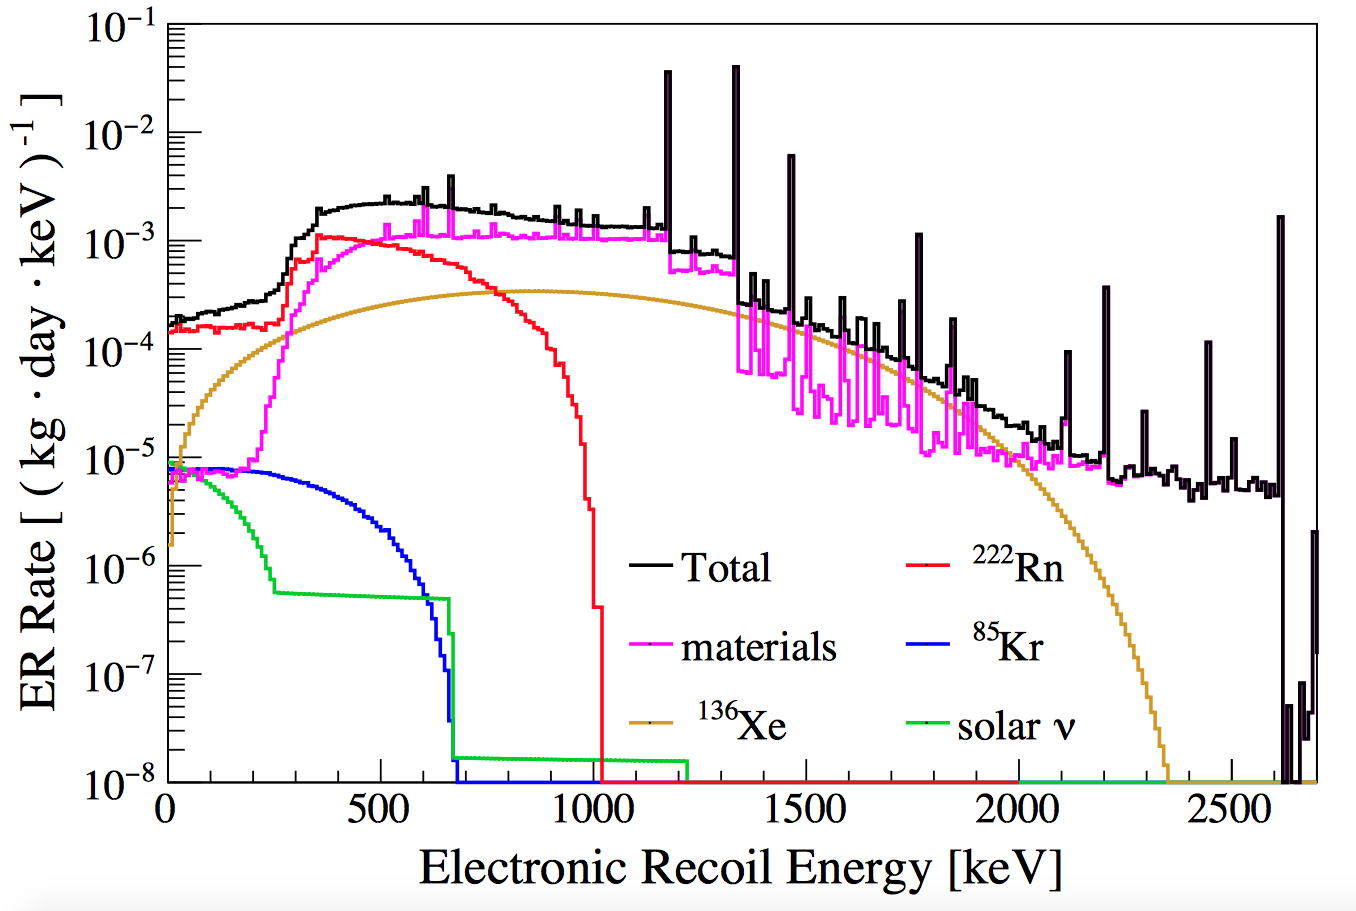
\includegraphics[height=5cm]{ERRateMCFull}
    \end{subfigure}%
    \begin{subfigure}[t]{0.5\textwidth}
        \centering
        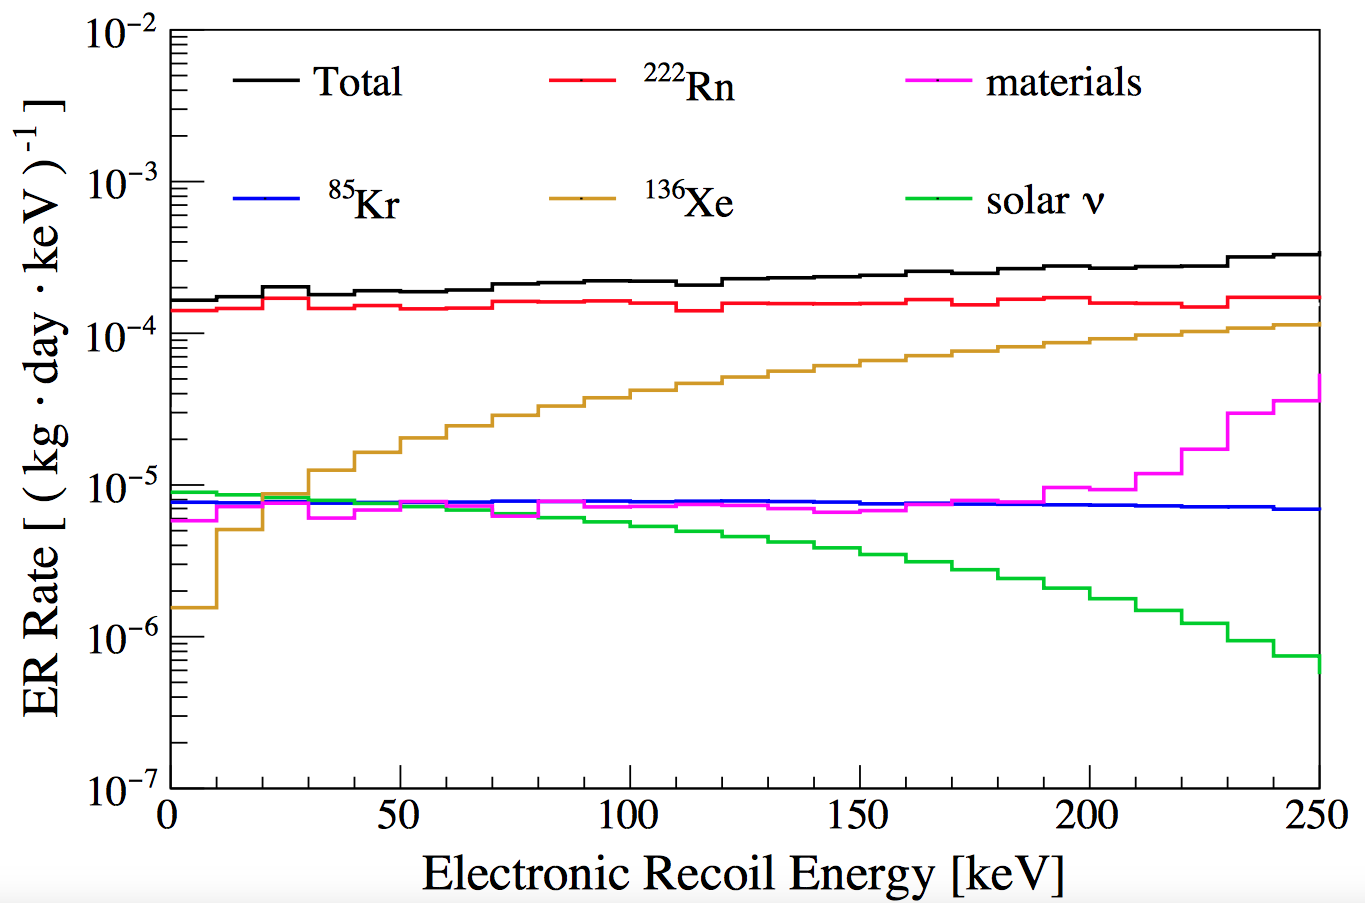
\includegraphics[height=5cm]{ERRateMCZoomed}
    \end{subfigure}
    \caption{Predicted electronic recoil energy background spectrum in a 1 t fiducial volume from Monte Carlo.  The left panel gives the
    ER expectation from 0 to $> 2614.5\ \mathrm{keV}$ (\ce{^{208}Tl}).  The right panel examines the 0-250 keV range.  Predictions can
    be compared to combined energy spectrum in \figref{fig:calibrations_photon_charge_efficiences_ces}.  Image credit:
    \citeref{Aprile2016a}.}
	\label{fig:backgrounds_er_spectrum}
\end{figure}



\subsubsection{\ce{^{136}Xe}}
\label{subsubsec:backgrounds_electronic_xe}
\ce{^{136}Xe} is the only unstable isotope of natural xenon.  It undergoes $2 \nu \beta^- \beta^-$ decay with
$t_{1/2} = 2.17 \times 10^{21}\ \mathrm{years}$ (\citeref{Albert2014}) and a Q-value of 2458 keV.  Because of its abundance in natural
xenon (\ce{^{136}Xe}/\ce{Xe} = 8.9\%) its presence is unavoidable.  At the scale of XENON1T it is subdominant - only responsible for
${\sim}2 \%$ of the total ER background, as seen in \figref{fig:backgrounds_er_spectrum} (right).  However, as detectors continue to grow
it will become more consequential.



\subsubsection{Solar Neutrinos}
\label{subsubsec:backgrounds_electronic_solar_neutrinos}
Solar neutrinos can elastically scatter off electrons, causing low-energy electronic recoils.  The recoil spectrum is the green line in
\figref{fig:backgrounds_er_spectrum}.  As with the \ce{^{136}Xe} $2 \nu \beta^- \beta^-$
decay its contribution is small, but as an irreducible background it will become more problematic as detectors grow.



\subsection{Nuclear Recoils}
\label{subsec:backgrounds_nuclear}
The nuclear recoil background comes from neutrons and neutrinos.  Whereas \gammarays are stopped within several cm, high-energy neutrons
have mean free paths of ${\sim}10\ \mathrm{cm}$, allowing them to move through the LXe volume more easily and having a higher probability
of scattering inside the FV.  Neutrinos move freely and cannot be shielded.  The nuclear recoil background is composed of
radiogenic and muon-induced neutrons as well as astrophysical neutrinos.



\subsubsection{Radiogenic Neutrons}
\label{subsubsec:backgrounds_nuclear_radiogenic}
Radiogenic neutrons are produced by primordial decay chains \ce{^{238}U}, \ce{^{235}U} and \ce{^{232}Th} in detector materials
(see \secref{subsec:backgrounds_detector_materials} for discussion on electronic and $\alpha$ recoils).  They are released in
$(\alpha, \mathrm{n})$ reactions that result from $\alpha$-emissions along the decay chains, as well as spontaneous fission (SF).  For
heavier nuclei radiogenic neutrons are generated almost exclusively by SF as the $(\alpha, \mathrm{n})$ reaction is suppressed by the
large Coulomb barrier (\citeref{Aprile2016a}).

\figref{fig:backgrounds_nuclear_radiogenic_rates} shows the neutron yield as a function of energy for PTFE and copper from Monte Carlo
predictions.  The \ce{^{238}U} and \ce{^{232}Th} chains are
separated at \ce{^{226}Ra} and \ce{^{228}Th} to account for the disequilibrium in decay rate
that is observed.  The PTFE has on average a lighter $Z$ than the copper, giving it a larger $(\alpha, \mathrm{n})$
contribution.  \figref{fig:backgrounds_nuclear_muon_induced_nr_rate} hows that for $E \gtrsim 3\ \mathrm{keV}$
radiogenic neutrons are the dominating contribution for the NR backgrounds.  The expected rate for 1 ton is
$0.6 \pm 0.1\ \mathrm{y^{-1}}$ (\citeref{Aprile2016a}).

\begin{figure}
    \centering
    \begin{subfigure}[t]{0.5\textwidth}
        \centering
        \includegraphics[height=5cm]{neutronyield-ptfe-v2}
    \end{subfigure}%
    \begin{subfigure}[t]{0.5\textwidth}
        \centering
        \includegraphics[height=5cm]{neutronyield-cu-v2}
    \end{subfigure}
    \caption{PTFE (left) and copper (right) differential yields for radiogenic neutrons per decay of parent nucleus.  Dashed lines show
    the contributions of spontaneous fission-only while solid show SF and $(\alpha, \mathrm{n})$ reactions.  Decays are shown
    for $\mathrm{^{238}U} \rightarrow \mathrm{^{230}Th}$ (black), $\mathrm{^{235}U} \rightarrow \mathrm{^{207}Pb}$ (red),
    $\mathrm{^{226}Ra} \rightarrow \mathrm{^{206}Pb}$ (green), $\mathrm{^{232}Th} \rightarrow \mathrm{^{228}Ac}$ (blue), and
    $\mathrm{^{228}Th} \rightarrow \mathrm{^{208}Pb}$ (pink).  Image credit: \citeref{Aprile2016a}.}
	\label{fig:backgrounds_nuclear_radiogenic_rates}
\end{figure}



\subsubsection{Muon Induced Neutrons}
\label{subsubsec:backgrounds_nuclear_muon_induced}
Cosmic muons interacting with the rock above the detector can produce up to GeV neutrons.  Such high-energy neutrons have a large mean
free path and it is possible they pass through the water shield (\secref{subsec:xenon1t_water_shield}).  However, simulations show that
if the associated showers from the muon interaction also enter the tank the tagging efficiency is $> 70\%$.  The predicted rate is
$< 0.01\ \mathrm{y^{-1}}$ for 1 t and is represented by the blue line in \figref{fig:backgrounds_nuclear_muon_induced_nr_rate}.

\begin{figure}
\centering
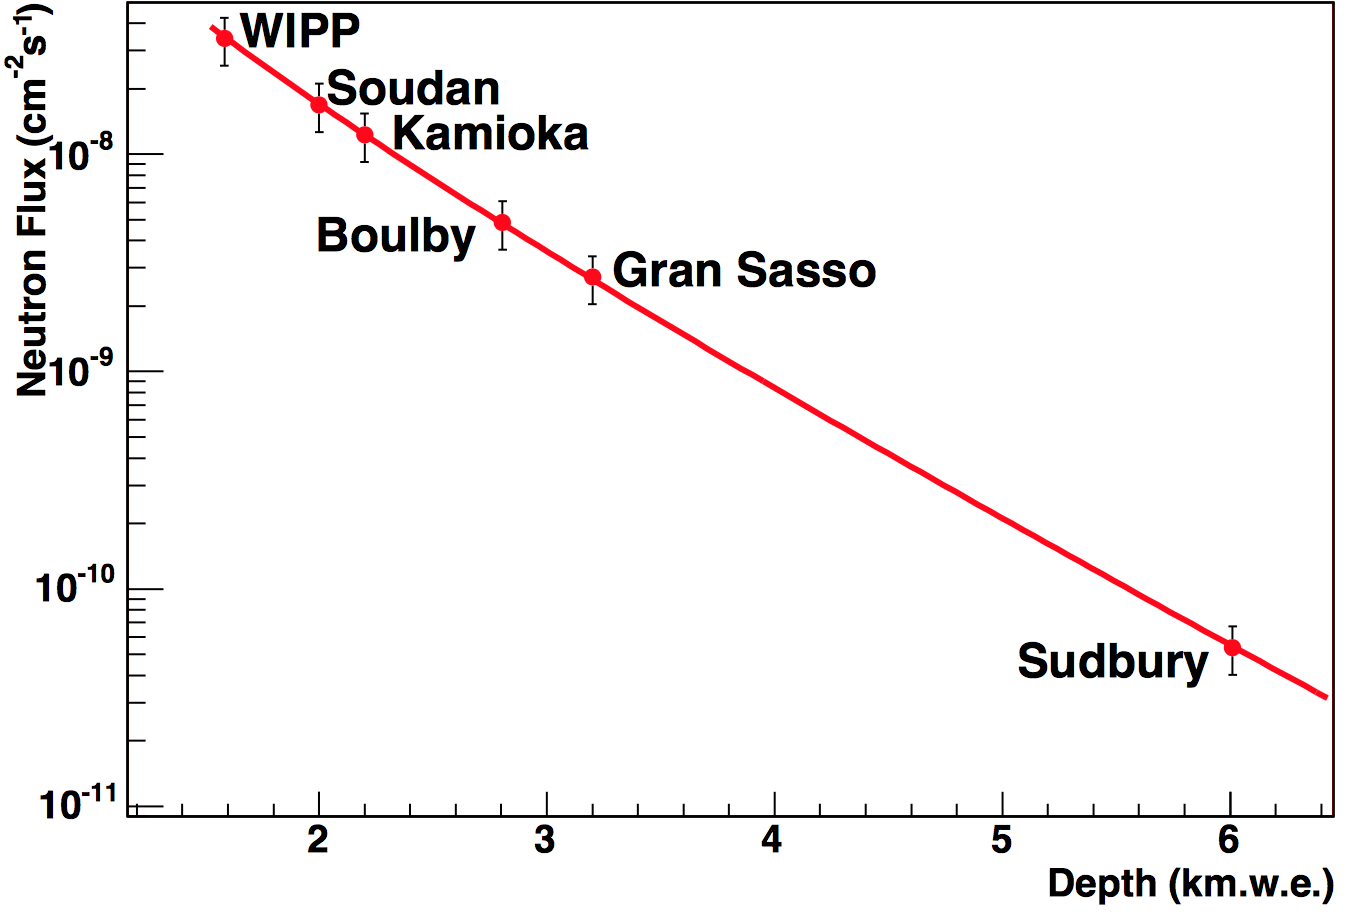
\includegraphics[width=0.6\textwidth]{MuonFluxOverDepth}
\caption{Neutron flux for WIPP, Soudan, Kamioka, Boulby, Gran Sasso, and Sudbury.}
\label{fig:backgrounds_nuclear_muon_induced_flux}
\end{figure}

\begin{figure}
\centering
\includegraphics[width=0.6\textwidth]{totalnrbackground}
\caption{Energy spectrum of the nuclear recoil background in the 1 t FV broken down by component.  Image credit: \citeref{Aprile2016a}.}
\label{fig:backgrounds_nuclear_muon_induced_nr_rate}
\end{figure}



\subsubsection{Neutrinos}
\label{subsubsec:backgrounds_nuclear_neutrinos}
The final contribution to the NR background comes from neutrinos that participate in coherent neutrino-nucleus scattering.  The primary
contributor to the integrated NR rate is solar \ce{^{8}B}, which is orders of magnitude larger than other sources and dominant at
recoil energies $< 3\ \mathrm{keV}$.  Solar $hep$, atmosphere, and diffuse supernova neutrinos also contribute.  We can see in
\figref{fig:backgrounds_nuclear_muon_induced_nr_rate} that neutrinos are the principal concern for recoils at $< 3\ \mathrm{keV}$.  The
number of detected events at $> 1\ \mathrm{keV}$ was predicted to be ${\sim} 90\ \mathrm{t^{-1}\ y^{-1}}$.  While this is below our
threshold, Poissonian variations may put a small fraction into our detection region.  By looking at the expected number of events closer
to our threshold (${\sim} 4\ \mathrm{keV}$) this drops to $1.8 \times 10^{-2}\ \mathrm{t^{-1}\ y^{-1}}$.  As mentioned in
\secref{subsubsec:backgrounds_electronic_solar_neutrinos} neutrinos will compose a greater fraction of our background in larger detectors
due to the inability to shield them.



\subsection{Detector Materials}
\label{subsec:backgrounds_detector_materials}
Detector materials were screened before purchasing (\secref{subsec:xenon1t_pmts, xenon1t_cryo}) to ensure
those with the lowest radioactivity were chosen.  The high self-shielding of LXe prevents the radiation from penetrating deep into
the detector, stopping the majority within several cm.  Still, it is important to understand our background for a number of reasons.  The
first is we want to maximize our FV.  But because including these events can affect our sensitivity we need to know
what ``safe distances'' from the top, bottom, and wall are.  The second is once we choose the FV it is important to have a reliable
estimate
of the number of events that will ``leak" into our FV, known as ``leakage events".  Failing to have an accurate prediction can result in
a sensitivity loss.  A third reason is these events can be used to characterizethe detector.

The primary isotopes from materials that play a role in our background are \ce{^{40}K}, \ce{^{60}Co}, \ce{^{235}U}, and the decay chains
of and \ce{^{238}U}, \ce{^{232}Th}, \ce{^{228}Th}, and \ce{^{226}Ra}.  In fact, although \ce{^{226}Ra} and \ce{^{228}Th} are part of the
\ce{^{238}U} and \ce{^{232}Th} chains, the disequilibrium between them prompts separation to
$\mathrm{^{238}U} \rightarrow \mathrm{^{230}Th}$ and $\mathrm{^{226}Ra} \rightarrow \mathrm{^{206}Pb}$ for \ce{^{238}U}, and
$\mathrm{^{232}Th} \rightarrow \mathrm{^{228}Ac}$ and $\mathrm{^{228}Th} \rightarrow \mathrm{^{208}Pb}$ for \ce{^{232}Th}.  The full
\ce{^{238}U} and \ce{^{232}Th} chains can be seen in \figref{fig:backgrounds_decay_chains}.

\begin{figure}
    \centering
    \begin{subfigure}[t]{0.5\textwidth}
        \centering
        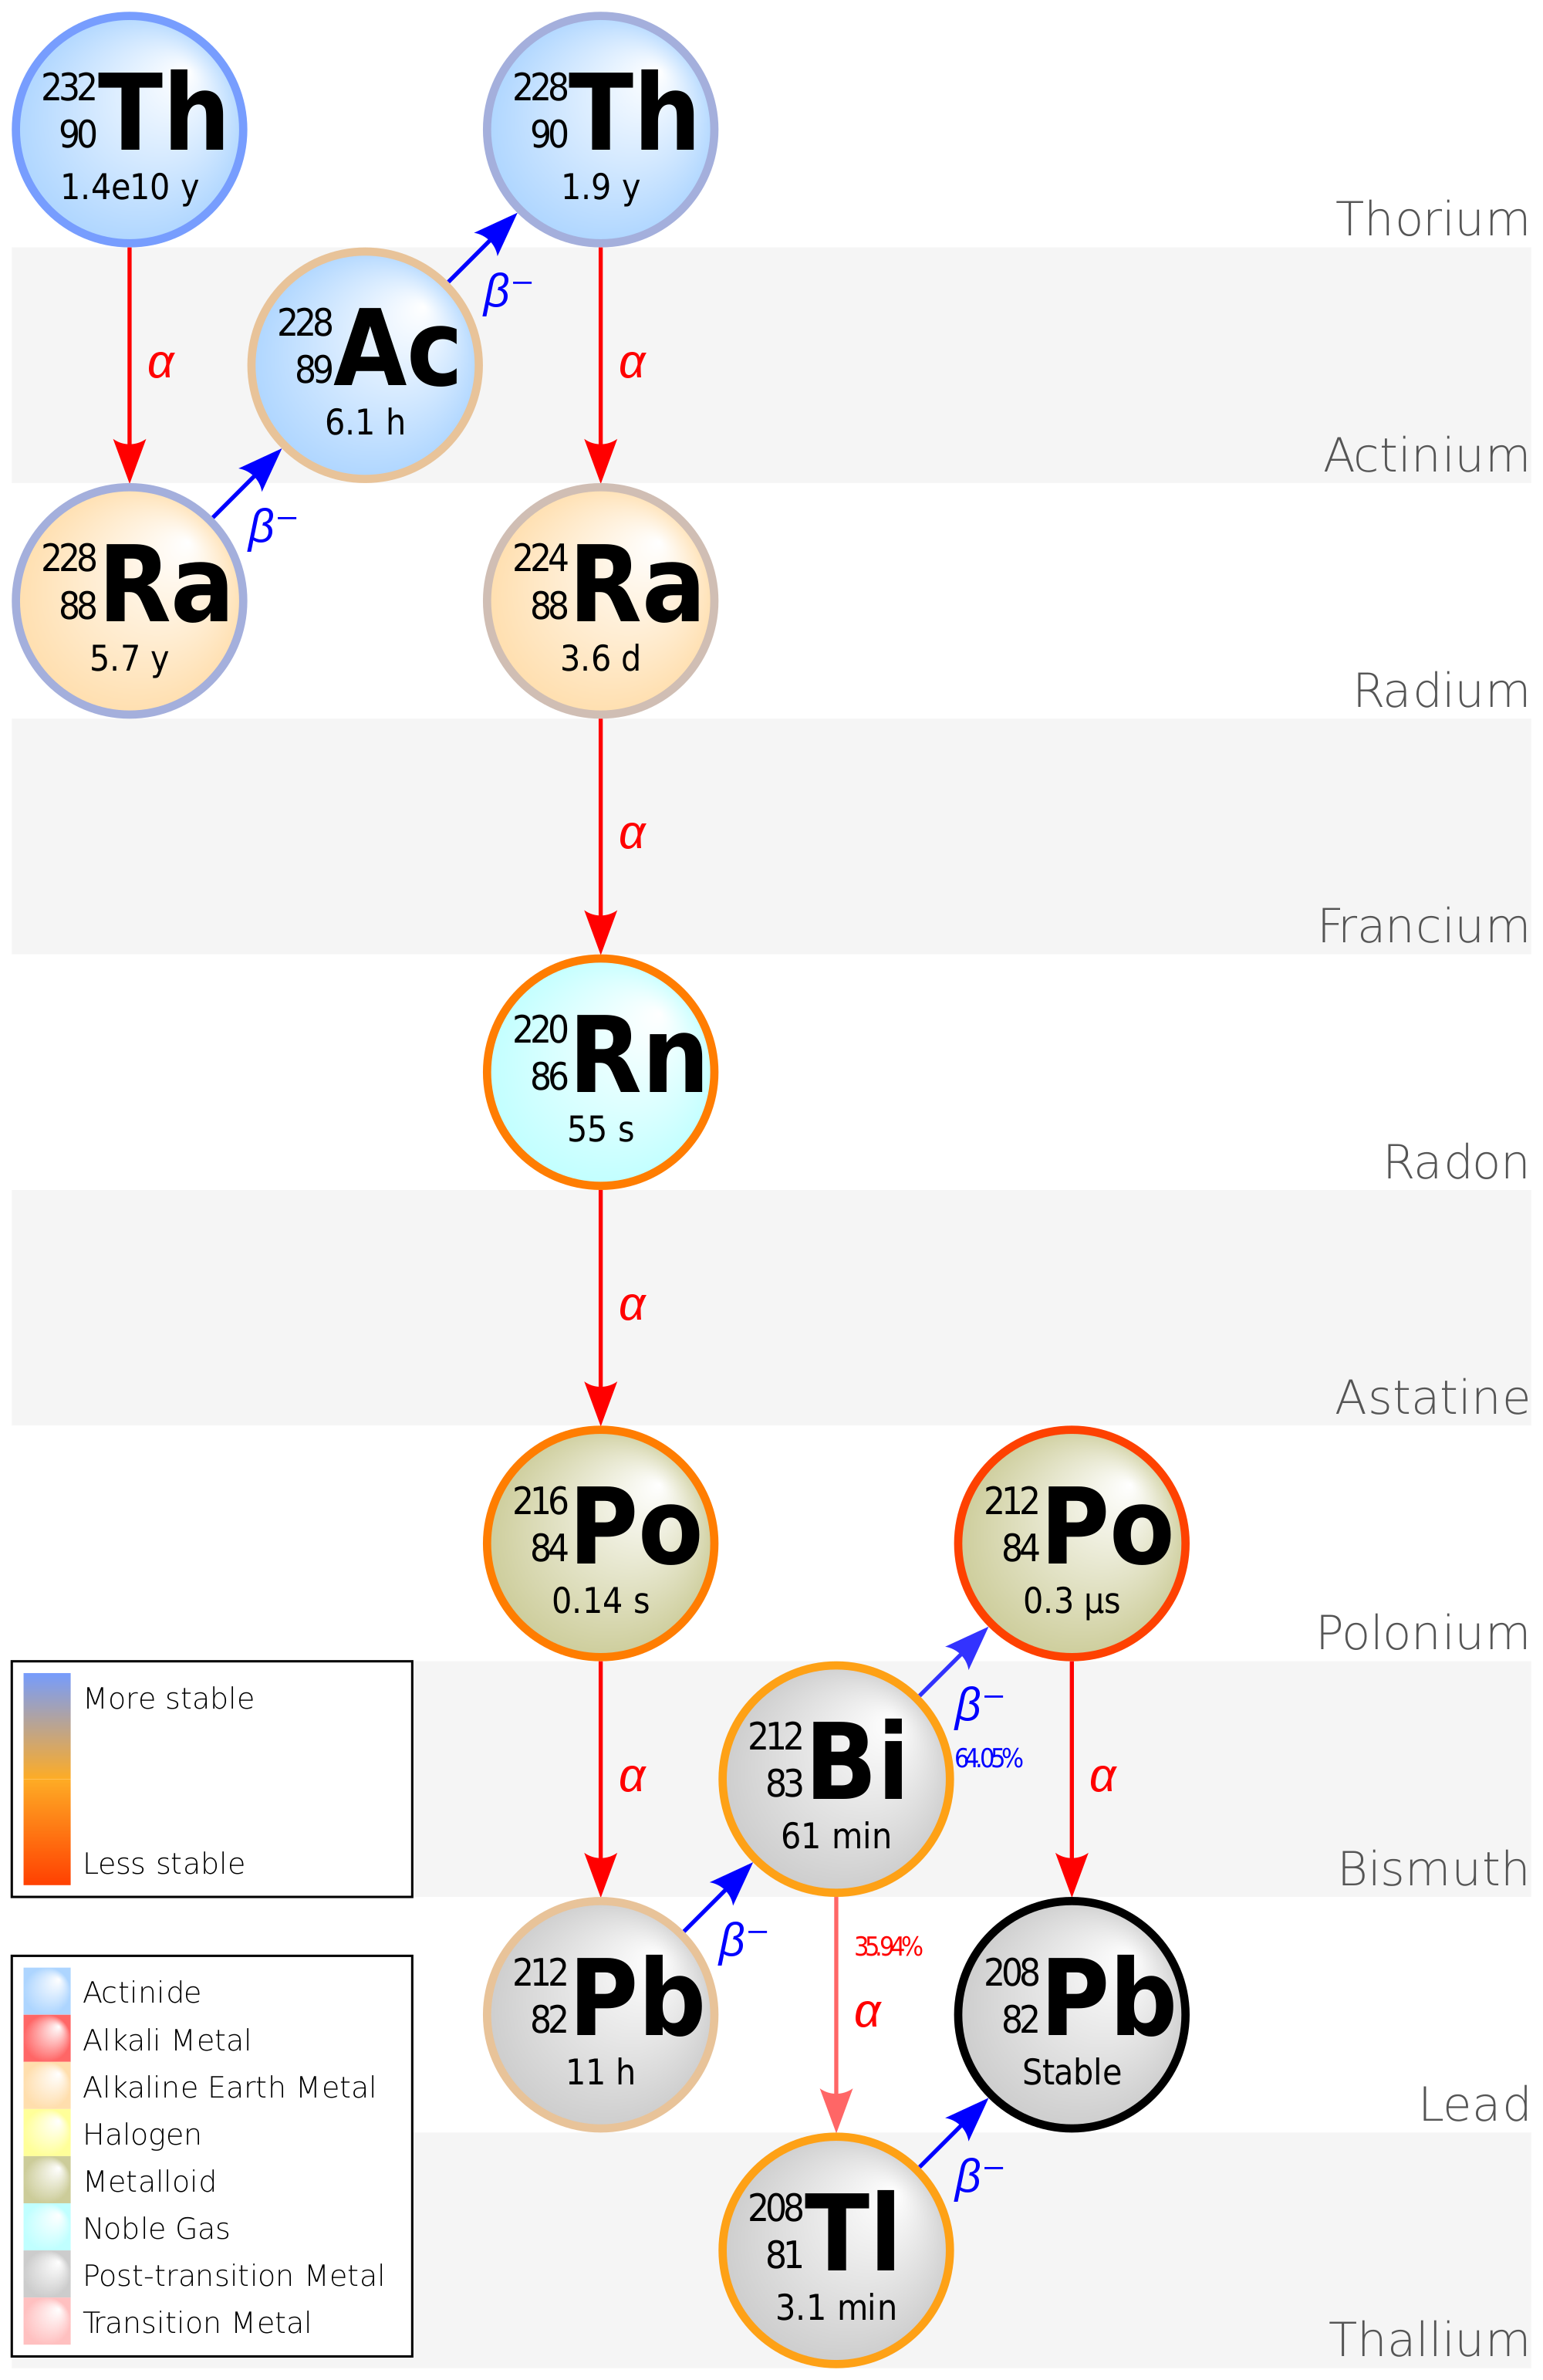
\includegraphics[width=\textwidth]{Decay_Chain_of_Thorium-232}
    \end{subfigure}%
    \begin{subfigure}[t]{0.5\textwidth}
        \centering
        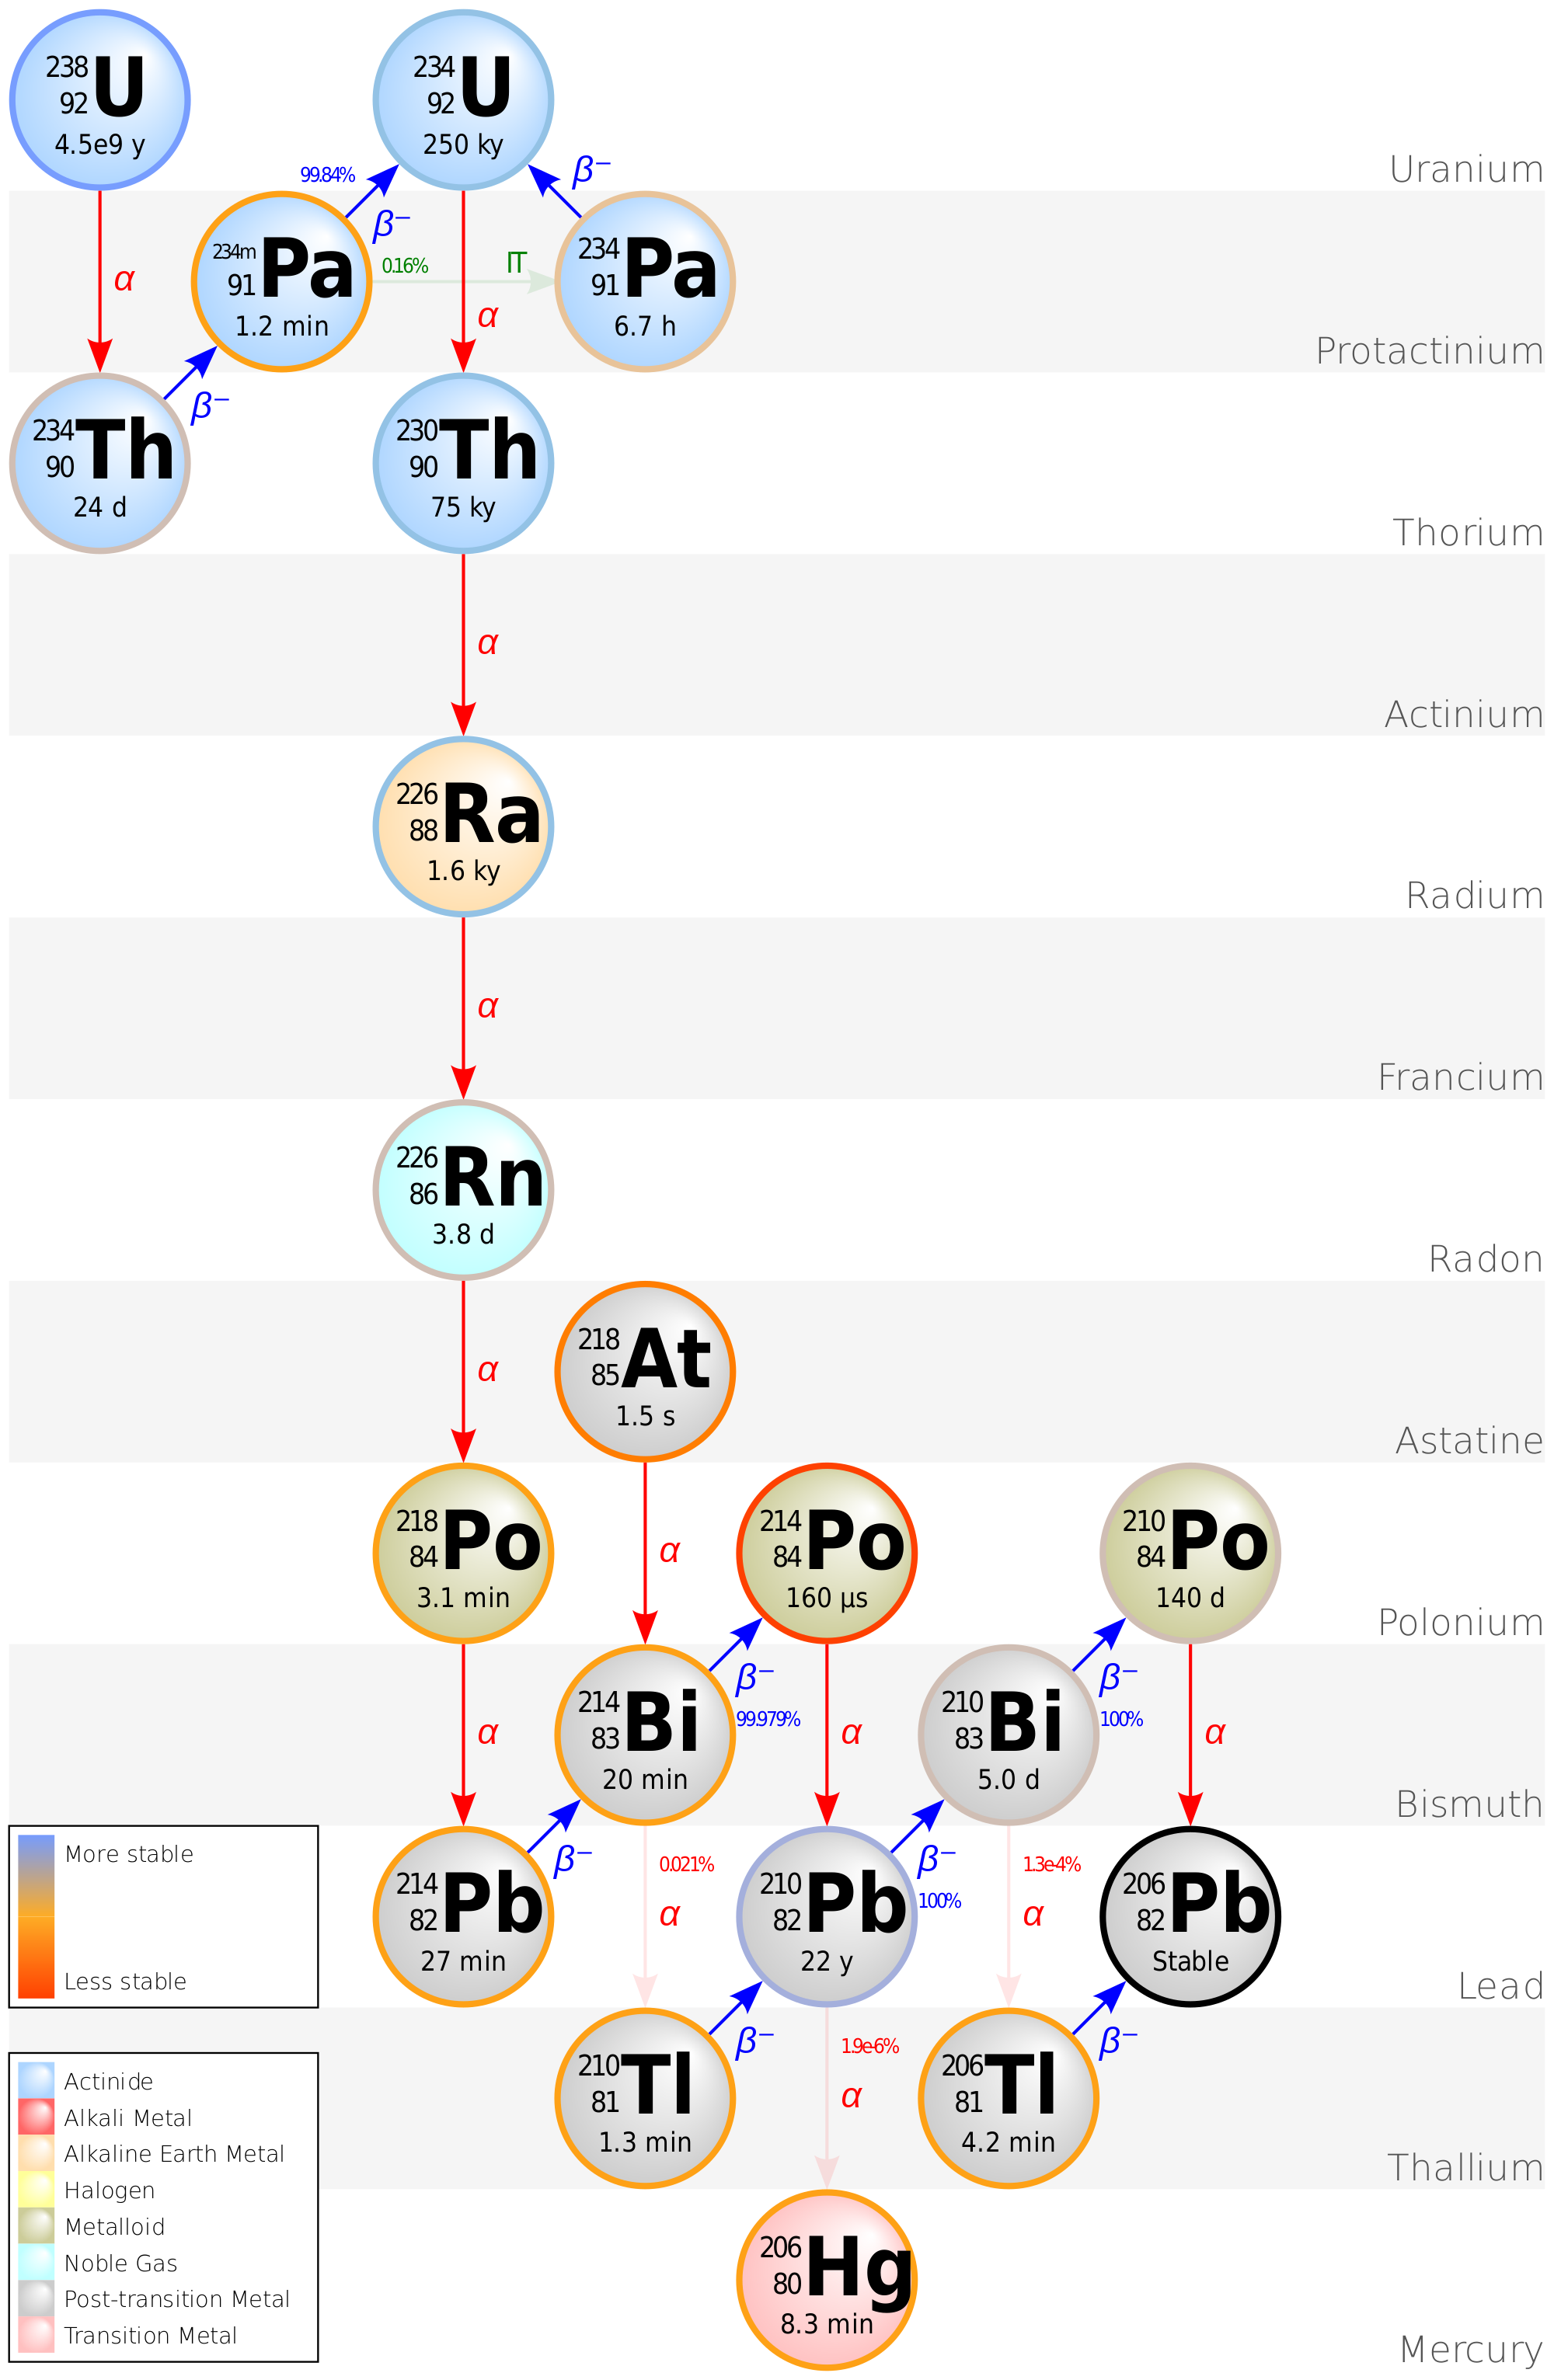
\includegraphics[width=\textwidth]{Decay_Chain_of_Uranium-238}
    \end{subfigure}
    \caption{Decay chains for \ce{^{232}Th} (left) and \ce{^{238}U} (right).  Image credit: \citeref{Wikimedia2018a, Wikimedia2018b}.}
	\label{fig:backgrounds_decay_chains}
\end{figure}

As \electron from wall events drift to the surface, a fraction will attach to the PTFE.  This decrease in S2 causes three main effects: 1)
an increase in position reconstruction uncertainty, 2) leakage into the NR band, and 3) small changes to the electric field.

A major constraint on the radius of our fiducial volume is the radioactivity from the PTFE panels - both the rate and reconstructed
positions, the latter of which has significant uncertainty at $\mathrm{S2_b} \lesssim 1000\ \mathrm{PE}$
(\figref{fig:calibrations_position_reconstruction_res}).  This makes \ce{^{210}Pb} on the PTFE panels concerning since its \betadecay has
a Q-value of just $63.5\ \mathrm{keV}$ and electron loss could result in a seemingly normal NR event inside our FV.  Moreover, despite a
chemical cleaning process during commissioning, a large amount of \ce{^{210}Pb} is known to be present from observations of its progeny
\ce{^{210}Po} $\alpha$-decays.  With a half-life of $t_{1/2} = 22.1\ \mathrm{y}$ and the continual addition of \ce{^{222}Rn}
(\secref{subsubsec:backgrounds_electronic_radon}), which decays to \ce{^{210}Pb} within days, the background rate will be
constant over the lifetime of the detector.

To address the first two points we model our expected contamination with events whose positions are reconstructed outside the
TPC ($r > 47.9\ \mathrm{cm}$).  The S2, cS1, cS2$_{\mathrm{b}}$, and $z$
distributions were found to be symmetric inside and outside the TPC, which was expected since the S2 was detected at the boundary and
inward and outward reconstruction are equally likely.  The
$r > 47.9\ \mathrm{rm}$ data was unblinded and the energy distribution was obtained via a fixed kernel density estimator (KDE) using
superposition of gaussians for each point in S2, cS1, cS2$_{\mathrm{b}}$, and $z$ space.

\begin{figure}
\centering
\includegraphics[width=\textwidth]{wall_leakage}
\caption{Science Run 1 background events.  Evens are plotted in $r \mdash z$ ($r^2 \mdash z$) in the left panel.  By selecting events
inside the 1.3
t fiducial volume (blue) the background rate decreases by more than a factor of 200.  Wall events are reconstructed symmetrically
about the TPC boundary due to imperfect position reconstruction resolution (\secref{subsec:det_char_position_reconstruction}), with the
exception of $z \gtrsim 10\ \mathrm{cm}$ where events from PMTs and other materials occur at smaller $r$.  $x \mdash y$ position are shown
in
the right plot with the colors corresponding to $\mathrm{log}_{10}(\mathrm{cS2_b / cS1})$.  Events in the center are the electronic recoil
background.  Events along the walls lose charge as they drift,
resulting in an under-corrected $\mathrm{S2_b}$ and can leak into the nuclear recoil band
($\mathrm{log}_{10}(\mathrm{cS2_b / cS1}) \approx 1.25 \mdash 2$).  The 1 t (green) and TPC boundary (black) are marked.  The color bar is
for the right panel only.}
\label{fig:backgrounds_detector_materials_wall_leakage}
\end{figure}

\begin{figure}
\centering
\includegraphics[width=0.8\textwidth]{surface_s2s1_distribution_blessed_sr1}
\caption{Expected surface background distribution in cS1-cS2$_{\mathrm{b}}$.  Electrons from wall events attach to the PTFE as they drift,
decreasing the S2 and potentially moving it into the NR band.  Projections are
shown for cS1 (top) and cS2$_{\mathrm{b}}$ (right) for all events in blue, and between the NR median (red dashed line) and
$-2 \sigma$ (solid black) in orange.  The surface background has the largest impact in our ROI at
$\mathrm{cS2_{\mathrm{b}}} \lesssim 400\ \mathrm{PE}$, $\mathrm{cS1} \lesssim 20\ \mathrm{PE}$.}
\label{fig:backgrounds_detector_materials_bands}
\end{figure}

The accumulation of charge on the PTFE panels was discovered by the author through tracking the \ce{^{222}Rn} and \ce{^{218}Po} decay
rates.  While the rate of events throughout the entire volume of the TPC was consistent, a radius cut-dependent rate was found.  This
is shown in \figref{fig:backgrounds_wall_charge}, where events reconstructed inside the designated radius (29, 32, 36.94, and 39 cm) are
plotted from February to September in SR1.  For $r < 29\ \mathrm{cm}$ limited statistics prevent precise measurements.

\begin{figure}
\centering
\includegraphics[width=\textwidth]{wall_charging_over_time}
\caption{\ce{^{222}Rn} and \ce{^{218}Po} decay rates ($R_{\mathrm{^{222}Rn}}$, $R_{\mathrm{^{218}Po}}$) from February-September 2017 for
radial cuts of 29, 32, 36.94, and 39 cm.  For all cuts $R_{\mathrm{^{222}Rn}} > R_{\mathrm{^{218}Po}}$ and
$dR_{\mathrm{^{222}Rn}}/dt > dR_{\mathrm{^{218}Po}}/dt$, though the latter converge at larger radii.  The increase is caused by \electron
buildup on the teflon that pushes events in the $-\hat{r}$ direction.  Residuals (in same units) show no bias from fits.}
\label{fig:backgrounds_wall_charge}
\end{figure}

The decay rates $R$ grow over time, with larger $r$ corresponding to greater increase.  One possibility might be a leak - for
which there may be other evidence (\secref{subsubsec:backgrounds_electronic_krypton, subsec:electron_lifetime_model_outgassing}) - but the
short half-lifes of \ce{^{222}Rn} and \ce{^{218}Po} demand the leak to be growing, which is in disagreement.  Additionally, a growing
leak should increase the decay rate across the entire detector, which is not observed.  This does not disqualify a constant leak since
the decay rates would be elevated but unchanging but does not explain \figref{fig:backgrounds_wall_charge}.

A second explanation is charge buildup on the PTFE.  Drifting \electron from events near the wall that attach to the PTFE will slowly
alter the electric field, primarily in the $\hat{r}$ direction.  The cumulative decay rate would not be impacted but events will move
further inward as this effect becomes stronger.  Furthermore, the rate of increase should grow with radius as the field distortion
becomes more significant, until it reaches a point where more events are lost than gained.  39 cm should be too far from the wall
to see a decrease in events, so
\figref{fig:backgrounds_wall_charge} supports the charge buildup conclusion as the slope for each fit grows with $r$.  The
decay rates differ because \ce{^{218}Po} may be left in a charged state following the decay of \ce{^{222}Rn} and pulled out of the
FV, which is evident when comparing the $z$-distributions.

\begin{figure}
\centering
\includegraphics[width=0.8\textwidth]{wall_charging_radius}
\caption{Decay rate increase (\figref{fig:backgrounds_wall_charge}) dependence on $r^2$.  Larger radii produce a bigger rate increase due
to proximity to the wall.  This helps estimate the scale of $dR/dt$ when selecting the FV.}
\label{fig:backgrounds_detector_materials_wall_charge_radius}
\end{figure}

\figref{fig:backgrounds_detector_materials_wall_charge_radius} shows the expected rate increase dependence on $r^2$ using the best-fit
values from \figref{fig:backgrounds_wall_charge}.  Both figures
raise the concern that the FV will grow over time as more events are pushed inwards.  To account for this a time-dependent position
reconstruction (\secref{subsec:det_char_position_reconstruction}) model is developed.

At $E \gtrsim 500\ \mathrm{keV}$ the background contribution becomes dominated by detector materials, with the exception of
${\sim} 1400 \mdash 2100\ \mathrm{keV}$ where \ce{^{136}Xe} is slightly larger.  For the energy region for spin-independent WIMP dark
matter \ce{^{136}Xe} is outpaced by roughly two orders of magnitude by \ce{^{214}Pb} inside a 1 t
FV.  \figref{fig:backgrounds_er_spectrum} shows the predicted ER backgrounds using Monte Carlo.



\subsection{Accidental Coincidence}
\label{subsec:backgrounds_ac}
In certain cases we may not be able to observe both the S1 and S2.  Interactions with only an S1, or lone-S1 events, result almost
entirely from PMT dark rate pile-up at low energies and below-cathode scatters at higher energies.  Those with just an S2, or lone-S2
events, come from interactions near the cathode and gate where the large electric field can significantly quench the S1.  The lone-S2s
could at least in part be explained by \ce{^{210}Pb}, which given its presence on the PTFE panels, suggest it may also exist on the
electrodes.

Generally lone-S1 and lone-S2 events do impact our data, but occasionally if they occur close to one another can mimic a real event, known
as accidental coincidence (AC).  Because we cannot know which events are AC, those that pass our cuts 
(\secref{subsubsec:er_nr_calibrations_parameter_determ_cuts}) - including a shape cut for S1s to eliminate single electrons - end up
in our final dataset.  It is therefore important to calculate the
number of expected events and the distribution.  The rate of AC events is given by

\begin{equation}
R_{\mathrm{AC}} = R_{\mathrm{LS1}} \times R_{\mathrm{LS2}} \times t_{d, \mathrm{max}}
\label{eq:er_nr_calibrations_parameter_determ_additional_components_accidental_coincidence}
\end{equation}

\noindent where $R_{\mathrm{LS1}}$ and $R_{\mathrm{LS2}}$ are the lone-S1
and -S2 rates and $t_{d, \mathrm{max}}$ is the maximum TPC drift time.  S1s, especially at low energy, are too small to trigger the
DAQ.  Therefore, to calculate $R_{\mathrm{LS1}}$ we select higher energy good events that contain an S1 and S2, and search the region
before the primary S1.  This method makes two assumptions.  The first is that lone-S1s should be uncorrelated in time, and thus
distributed uniformly over large timescales.  The second is that the S1s we find do not have a complementary S2.  The former
seems reasonable since we do not expect PMT dark rates and below-cathode scatters to follow any pattern.  The latter is valid because
the probability of having two interactions in the same time window is negligible.

\begin{figure}
\centering
\includegraphics[width=0.8\textwidth]{ac_s2s1_distribution_blessed_sr1}
\caption{Expected accidental coincidence distribution in cS1-cS2$_{\mathrm{b}}$ space.  Isolated S1s and S2s are randomly coupled to
imitate real events in the TPC.  S1 and S2 corrections are applied and events that pass the cuts are plotted.  Projections are
shown for cS1 (top) and cS2$_{\mathrm{b}}$ (right) for all events in blue, and between the NR median (red dashed line) and
$-2 \sigma$ (solid black) in orange.  The majority of events in the reference region are in $\mathrm{cS1} \lesssim 10\ \mathrm{PE}$,
$\mathrm{cS2_b} \lesssim 500\ \mathrm{PE}$.}
\label{fig:er_nr_calibrations_parameter_determ_ac}
\end{figure}

Accidental coincidences do not benefit from fiducialization like much of our other background.  In fact,
\eqnref{eq:er_nr_calibrations_parameter_determ_additional_components_accidental_coincidence} shows $R_{\mathrm{ac}}$ increases
with detector size.  Still, its total contribution is comparatively small to the total background.  AC is source or background-dependent,
so for this analysis
distributions for \ce{^{220}Rn}, $\mathrm{^{241}AmBe}$, and NG data were each included in the electronic and nuclear recoil band fitting
(\secref{sec:er_nr_calibrations}).  Similar conditions and durations meant the SR0 and SR1 $^{241}$AmBe calibrations had nearly the same
AC expectation so it was not
necessary to include independent distributions; however, SR0 and SR1 AC \ce{^{220}Rn} were sufficiently different and required independent
inputs.  \figref{fig:er_nr_calibrations_parameter_determ_ac} shows the expected AC distribution in cS1-cS2$_{\mathrm{b}}$ space
with the region of interest marked by dotted red (median) and solid black ($-2 \sigma$) lines.




\section{Electronic and Nuclear Recoil Bands}
\label{sec:er_nr_calibrations}
To differentiate the nuclear from electronic recoil bands respective calibrations are performed and fit.  These are critical as
they define the reference region and discrimination power between potential WIMPs and background.  \ce{^{220}Rn} calibrations are used for
the ER band and are are performed regularly.  For NR \ce{^{241}AmBe} and a deuterium-deuterium
neutron generator (NG) are used, both of which are positioned in the water tank outside the cryostat.  \ambe calibrations are done in
SR0 and SR1 and a NG calibration is performed in SR1.

For this analysis all five sets of calibration data from both science runs were fit simultaneously.  This was
significant because it forced values that are common to some or all of the calibrations (e.g. $W$, $p_{\mathrm{dpe}}$, etc. are shared
between all five, while $g_1$, $g_{2\mathrm{b}}$, etc. are shared within science runs) to converge to a single
value.\footnote{for First Results
the \radoncal and \ambe were independently fit.}  \tabref{tab:er_nr_calibrations_parameters} lists the variables included in the fit and
to which calibrations they apply.



Beginning with the physical processes from the interaction itself to the final values of cS1 and \cstwob the fit is
possible by running on GPUs, which provide a $10^{2 \mdash 3}$ times speed increase.



\subsection{Purpose of Calibrations}
\label{subsec:er_nr_calibrations_purpose}
The electronic and nuclear recoil calibrations define a probability density function (PDF)
such that for any event we can quantify the likelihood of what caused it, giving improved sensitivity over
purely statistical approaches (\secref{sec:direct_detect}).  Doing so requires a complete understanding of the TPC background, which
in addition to nominal electronic recoils includes wall leakage (\secref{subsec:backgrounds_detector_materials}) and accidental
coincidence (\secref{subsec:backgrounds_ac}).  It also demands that
the physical processes that occur starting from the exciton-ion ratio through the data acquisition are correctly modeled and able to be
simulated on a reasonable time scale.

Following the ER and NR fits a signal PDF is generated.  For this analysis the
signal is a WIMP but in general it is not constrained to this.  The shape of the PDF depends on the WIMP mass.  The data can be compared
to the PDF for a given WIMP mass and cross-section to see how well it agrees with a signal.  A limit is set if all cross-sections below
some value match the data, while a discovery can be claimed if the data prefers a particular mass and cross-section over others.

\figref{fig:er_nr_calibrations_purpose_wimp_contours} shows the background model with contours for 6, 50 and 1000 GeV WIMPs overlaid from
First Results.  The ER band is the bright yellow region and the horizontal band around $\mathrm{cS2_b} = 150\ \mathrm{PE}$ is accidental
coincidence.  The overlap between signal and background emphasizes the importance of electronic and nuclear recoil band
fitting.  An incorrect fit can shift the positions of the bands, changing our understanding of the origin of events.

\begin{figure}
\centering
\includegraphics[width=\textwidth]{wimp_contours}
\caption{Total background model from First Results with 50, 90, and 99\% contours for 6 (left), 50 (center), and 1000 (right) GeV
WIMPs.  The bright yellow region is the
electronic recoil band, which was fit using a similar method to this section.  Accidental coincidence is visible as the horizontal strip
around $\mathrm{cS2_b} = 150\ \mathrm{PE}$.  The region of expected signal changes with WIMP mass.}
\label{fig:er_nr_calibrations_purpose_wimp_contours}
\end{figure}



\subsection{Parameter Determination}
\label{subsec:er_nr_calibrations_parameter_determ}
This approach compares the distributions of Monte Carlo events with the data.  Because of the nearly flat distribution of events at
relevant
energies along with homogenous distribution, Monte Carlo features $E_{\mathrm{true}}$, $x_{\mathrm{true}}$, $y_{\mathrm{true}}$,
$z_{\mathrm{true}}$, for \ce{^{220}Rn} are randomly sampled from a
uniform distribution.  \ce{^{241}AmBe} and neutron generator Monte Carlo are simulated using GEANT4, and include the number of
scatters for each neutron.  The $\beta^-$ from \ce{^{220}Rn} should not scatter so this is fixed to 1.  These values represent the
``truth'' information - that is, these are the true interaction values and are inputs for the fits.  Reconstructed $x \mdash y$ values
will be referred to as $x_{\mathrm{rec}}$
and $y_{\mathrm{rec}}$ (energy and depth will be denoted $E$ and $z$ and are equivalent in the fast-MC to the truth values).

\figref{fig:er_nr_calibrations_parameter_determ_flow_chart} shows the flow chart for the band matching.  Each Monte Carlo event is run
through a series of events that mimic the expected sequence as closely as possible.  The parameters used in this estimation come from
a variety of sources including physical properties reported from literature and detector characterization measurements
(\secref{sec:det_char}).  The process takes the simulated energy from a Monte Carlo event and outputs observables cS1 and
$\mathrm{cS2_b}$.  These in turn are binned in cS1-$\mathrm{log_{10}(cS2_b / cS1)}$ space, and the likelihood for equivalent bins
between data and MC is calculated (\secref{subsubsec:er_nr_calibrations_parameter_determ_mc_match}).  To describe our energy region of
interest as well as possible only events with $0 \leq \mathrm{cS1} \leq 100$ and $0.5 \leq \mathrm{log_{10}(cS2_b / cS1)} \leq 3.5$ are
considered.  As the parameters vary the likelihood will increase or decrease, allowing a minimizer to find the best-fit values.

\begin{figure}
\centering
\includegraphics[width=\textwidth]{FlowChart}
\label{fig:er_nr_calibrations_parameter_determ_flow_chart}
\end{figure}

The conversion of truth MC to cS1 and \cstwob is referred to as a ``fast MC'' (random numbers are drawn from probability distributions to
select sets of parameters).  ``Truth MC'' will refer to the simulated events before the fast MC ($E_{\mathrm{true}}$,
$x_{\mathrm{true}}$, $y_{\mathrm{true}}$, $z_{\mathrm{true}}$, and number
of scatters).  ``MC'' will denote the sum of all the fast MC components, usually in the form of a PDF (histogram), for
a single comparison with data.  Finally, a Markov Chain Monte Carlo (MCMC) is used to fit the data and Monte Carlo and the best-fit values
are derived from the posterior.  \secref{subsubsec:er_nr_calibrations_parameter_determ_er} (ER) and
\secref{subsubsec:er_nr_calibrations_parameter_determ_nr} (NR) discusses the physical steps that occur beginning with energy
deposition until final cS1 and $\mathrm{cS2_b}$ (and by extension the operations applied in the fast MC).

The number of fast-MC events simulated for each likelihood iteration is $\mathcal{O}(10^6)$.  A fast-MC event randomly selects one of the
truth input events.  Such large statistics are necessary for
convergence;
however, nominal running time is far greater than any sensible time-scale.  This was solved by using graphical processing units (GPUs),
which can run the events in parallel, providing a boost in speed of $10^{2 \mdash 3}$ times and reducing the required time to a
reasonable level.

The calibrations were fit in the First Results FV ($-92.9 < z < -9\ \mathrm{cm}$, $r_{\mathrm{rec}} < 36.94\ \mathrm{cm}$
\figref{fig:calibrations_position_reconstruction}) despite the 1.3 t fiducial mass used in this analysis.  This was done to minimize wall
events and contamination from materials at the top and bottom of the TPC (mainly PMTs).



\subsubsection{Electronic Recoils}
\label{subsubsec:er_nr_calibrations_parameter_determ_er}
The electronic recoil calibration is performed using \ce{^{220}Rn} (decay chain shown in the left panel of
\figref{fig:backgrounds_decay_chains}).  It is used because of the \ce{^{212}Pb} \betadecay with Q-value 569.9 keV and can be performed
as an internal calibration.  In the future we hope to use tritiated methane $\mathrm{C H_3 T}$, which undergoes \betadecay
with a maximum energy of 18.6 keV.  This would provide significantly more statistics in our region of interest in a short amount
of time.  However, as mentioned in \secref{subsubsec:xenon1t_calibrations_internal} $\mathrm{C H_3 T}$ has a half-life of 12.3 y and there
is concern it may attach to the cryostat.  For this reason we instead use \ce{^{220}Rn}, for which six separate calibrations were
performed during Science Run 1.

When energy is deposited in LXe a number of quanta will be produced.  For electronic recoils this follows the normal distribution

\begin{equation}
n_q \sim \mathrm{Norm} \bigg( \mu = \frac{E}{W},\ \sigma^2 = \frac{E F}{W} \bigg)
\label{eq:er_nr_calibrations_parameter_determ_er_quanta}
\end{equation}

\noindent where $F$ is the Fano Factor (\citeref{Fano1947}) discussed in \secref{sec:er}.  Its derivation and subsequent measurements
demonstrates
that fluctuations in $n_{\mathrm{q}}$ are smaller than a Poisson distribution, and it is estimated to be $F = 0.059$
(\citeref{Doke1976}).  For the
fast MC $F$ is fixed.  Although a later measurement found different best-fit values, their result was
compatible with \citeref{Doke1976} when including uncertainty (\citeref{Seguinot1995}).  $W$, the average energy to produce a single
quanta, is constrained by a Gaussian with $\mu = 13.7,\ \sigma = 0.2\ \mathrm{eV}$ following the measurement of \citeref{Dahl2009}.

For electronic recoils quenching is negligible so is not considered.  The quanta will be divided into excitons and electron-ion pairs
$n_q = n_{\mathrm{ex}} + n_{\mathrm{ion}}$ and will be divided according to a binomial distribution

\begin{equation}
n_{\mathrm{ion}} \sim \mathrm{Binom} \Bigg(n = n_{\mathrm{q}},\ p = \frac{1}{1 + \frac{n_{\mathrm{ex}}}{n_{\mathrm{ion}}}} \Bigg)
\label{eq:er_nr_calibrations_parameter_determ_er_nions}
\end{equation}

\noindent where $n_{\mathrm{ex}} / n_{\mathrm{ion}}$ is constrained $0.06 \mdash 0.2$ and expected to be energy independent
(\citeref{NEST2011}).  Some \electron will recombine with \ce{Xe^+} to form
excitons and emit photons as they decay to the ground state.  The recombination fraction $r$ depends on the field in the LXe and the
interaction energy, and has intrinsic fluctuations $\Delta r$ (\citeref{LUX2016, Aprile2018a}).  A truncated Gaussian is assumed

\begin{equation}
r \sim \mathrm{Norm} \Big( \mu = \langle r \rangle,\ \sigma^2 = (\Delta r)^2 \Big)
\end{equation}

\noindent where $0 \leq r, \Delta r \leq 1$ and is parameterized using a modified Thomas-Imel box model (\citeref{Thomas1987})

\begin{equation}
\langle r \rangle = \frac{1}{1 + e^{-(E - E_0) / E_1}}
\bigg( 1 - \frac{\mathrm{ln}(1 + n_{\mathrm{ion}} \varsigma / 4)}{n_{\mathrm{ion}} \varsigma / 4} \bigg)
,\ \ \varsigma = \gamma_{\mathrm{er}} e^{-E / \omega_{\mathrm{er}}} F_{\mathrm{E}}^{-\delta_{\mathrm{er}}}
\label{eq:er_nr_calibrations_parameter_determ_ti}
\end{equation}

\noindent for the fit.  Here $\varsigma$ has been adapted from \eqnref{eq:ti_recomb} to include a power law field-dependence to allow
simultaneous fitting of SR0 and SR1, and an exponential energy term to extend compatibility to high energy
(${\sim} 20\ \mathrm{keV_{ee}}$).  An energy-dependent Fermi-Dirac is used to suppress recombination at
$\lesssim 2\ \mathrm{keV_{ee}}$ for better agreement with data.  The parameters do not have priors and are constrained to
$0 \leq \gamma_{\mathrm{er}} \leq 0.5$, $0 \leq E_0, E_1 < \infty$, and
$-\infty < \omega_{\mathrm{er}}, \delta_{\mathrm{er}} < \infty$.

Recombination fluctuations are modeled as

\begin{equation}
\Delta r = A(1 - e^{-E/B})
\label{eq:er_nr_calibrations_parameter_determ_er_rec_fluctuations}
\end{equation}

\noindent where parameters $A,B > 0$ are allowed to vary freely.  The number of electron-ion pairs that recombine is

\begin{equation}
n_{\mathrm{rec}} \sim \mathrm{Binom} \big(n = n_{\mathrm{ion}},\ p = r \big)
\end{equation}

\noindent yielding a final number of photons and electrons

\begin{subequations}
\begin{align}
n_{\mathrm{ph}} &= n_{\mathrm{ex}} + r\, n_{\mathrm{ion}} \\
n_{\mathrm{e}} &= (1 - r) n_{\mathrm{ion}}
\end{align}
\end{subequations}

\noindent  As mentioned above \ce{^{220}Rn} is homogeneously spread throughout the TPC and has an energy spectrum that is nearly
flat between 0-30 keV so each event's truth energies and positions are randomly sampled from uniform distributions.



\subsubsection{Nuclear Recoils}
\label{subsubsec:er_nr_calibrations_parameter_determ_nr}
Two nuclear recoil sources were used for calibrations: americium beryllium (\ce{^{241}AmBe}) and a neutron generator
(NG).  \ambe was used once in both SR0 and SR1 and the NG was used in SR1.  \ambe decays to \ce{^{237}Np} by $\alpha$-emission and
the large \ce{^{9}Be} $\alpha$ cross-section prompts a second decay

\begin{equation}
\mathrm{^{9}Be} + \mathrm{^{4}He} \rightarrow \mathrm{^{12}C + n} + \gamma
\end{equation}

\noindent emitting a $< 11\ \mathrm{MeV}$ neutron.  The neutron generator (NSD Gradel Fusion NSD-35-DD-C-W-S) uses
deuterium-deuterium (D-D) fusion

\begin{equation}
\mathrm{^{2}D} + \mathrm{^{2}D} \rightarrow \mathrm{^{3}He} + \mathrm{n}
\end{equation}

\noindent where the \ce{^{3}He} and n are expelled at 0.82 and 2.45 MeV, respectively.  The energy spectrum can be seen in
\figref{fig:er_nr_calibrations_parameter_determ_nr_ng_energy}.  It shows two peaks - one at 2.2 MeV and the other at 2.7 MeV.  These
are the energies seen in the lab frame (2.45 MeV was in the deuteron's) and correspond to neutrons emitted at $180^{\circ}$ and
$0^{\circ}$, respectively.  The NG can operate at rates as low as $10\ \mathrm{n\ s^{-1}}$
and as high as $10^7\ \mathrm{n\ s^{-1}}$, which allows flexibility for our objectives.  A higher-energy neutron
population is produced by tritium via

\begin{figure}
\centering
\includegraphics[width=0.6\textwidth]{ng_energy_spectrum}
\caption{Simulated neutron energy spectra in fusion region of the NG (red dashed line) and at the pulse shape discriminator during
calibration (blue shaded region).  Deconvolution of data from calibration (black solid line) is also shown.  Spectra are normalized by
the 2.2-2.7 MeV range.  Image credit: \citeref{Lang2018}.}
\label{fig:er_nr_calibrations_parameter_determ_nr_ng_energy}
\end{figure}

\begin{equation}
\begin{aligned}
\mathrm{^{2}D} + \mathrm{^{2}D} &\rightarrow \mathrm{^{3}T} + \mathrm{p} \\
\mathrm{^{3}T} + \mathrm{^{2}D} &\rightarrow \mathrm{^{4}He} + \mathrm{n}
\end{aligned}
\end{equation}

\noindent that expels neutrons at 14.1 MeV.  The contribution of deuterium-tritium fusion was measured to be $3.5 \pm 0.2\%$ before
installation at LNGS (\citeref{Lang2018}).  Because the tritium is created in deuterium-deuterium fusion and has
$t_{1/2} = 12.3\ \mathrm{y}$ its fraction will increase with continued use.  For details on the characterization of the NG
please refer to \citeref{Lang2018}.

The positions for \ambe and NG events are shown in \figref{fig:er_nr_calibrations_parameter_determ_nr_ambe_positions} and
\figref{fig:er_nr_calibrations_parameter_determ_nr_ng_positions}.  Their ${\sim}10\ \mathrm{cm}$ mean free path causes clustering
in $r$ and $\phi$ closest to the calibration source.  Because we expect our
detector does not vary over $r$ and $\phi$ inside the 1 t FV the results of the lopsided position distribution are applied to the entire
active volume.  Events in the region furthest from the source are mostly background.  Fewer background events are present in the NG data
because of the shorter calibration time.  SR0 \ambe is not shown but its distribution of NR events is similar to
\figref{fig:er_nr_calibrations_parameter_determ_nr_ambe_positions} because the location of the source was the same.  Many more ER events,
however, were present since it was before the online distillation (\secref{subsec:xenon1t_kr_dist}).

\begin{figure}
\centering
\includegraphics[width=\textwidth]{ambe_positions}
\caption{Positions of events from SR1 \ambe calibration.  Events are clustered in the region of the detector closest to the \ambe
source.  The black line marks the 1 t fiducial volume.  Aside from the higher ER background, the SR0 distribution looks similar since the
source was at the same location inside water tank.}
\label{fig:er_nr_calibrations_parameter_determ_nr_ambe_positions}
\end{figure}

\begin{figure}
\centering
\includegraphics[width=\textwidth]{ng_positions}
\caption{Positions of events from SR1 neutron generator calibration.  Events are densely distributed in the region of the TPC closest to
the NG source.  The black line shows the 1 t fiducial volume.}
\label{fig:er_nr_calibrations_parameter_determ_nr_ng_positions}
\end{figure}

The microphysical processes that follow a nuclear recoil differ from ER (\secref{subsubsec:er_nr_calibrations_parameter_determ_er}).  As
discussed in \secref{sec:nr} a sizable portion of the energy is lost to atomic motion.  To model this we use the Lindhard theory
in \eqnref{eq:er_nr_calibrations_parameter_determ_nr_lindhard}.

\begin{subequations}
\begin{align}
\epsilon &= 11.5 \bigg( \frac{E}{\mathrm{keV}} \bigg) Z^{-7/3} \\
g( \epsilon ) &= 3 \epsilon ^{0.15} + 0.7 \epsilon ^{0.6} + \epsilon \\
L( \epsilon ) &= \frac{k g( \epsilon ) }{1 + k g( \epsilon )}
\end{align}
\label{eq:er_nr_calibrations_parameter_determ_nr_lindhard}
\end{subequations}

$k$ is the proportionality constant between the electronic stopping power and recoiling nucleus velocity.  The Lindhard factor
$L$ is the fraction of energy not converted to excitons or electron-ion pairs

\begin{equation}
n_{\mathrm{q}} \sim \mathrm{P} \bigg( \mu = \frac{E L}{W} \bigg)
\label{eq:er_nr_calibrations_parameter_determ_nr_quanta}
\end{equation}

\noindent that uses a Poisson distribution as an approximation.  In reality the track structure of nuclear recoils makes the true
distribution more complicated.  The number of ions is found in the same way as for
electronic recoils

\begin{equation}
n_{\mathrm{ion}} \sim \mathrm{Binom} \Bigg(n = n_{\mathrm{q}},\ p = \frac{1}{1 + \frac{n_{\mathrm{ex}}}{n_{\mathrm{ion}}}} \Bigg)
\end{equation}

\noindent and $n_{\mathrm{ex}} = n_{\mathrm{q}} - n_{\mathrm{ion}}$.  Recombination is given by

\begin{equation}
n_{\mathrm{rec}} \sim \mathrm{Binom} \big(n = n_{\mathrm{ion}},\ p = r \big)
\end{equation}

\noindent where $r$ described by the Thomas-Imel model without the Fermi-Dirac tuning

\begin{equation}
r = 1 - \frac{\mathrm{ln} (1 + n_{\mathrm{ion}} \varsigma)}{n_{\mathrm{ion}} \varsigma}
\end{equation}

\noindent where $\varsigma$ is field-dependent.  Unlike ER, no recombination fluctuations have been observed for nuclear recoils so
$\Delta r$ is not considered.  Biexcitonic quenching and Penning process, both of which decrease
$\mathrm{n_{ph}}$, must also be considered.  Biexcitonic quenching arises when two
\ce{Xe^{*}} interact to free an $e^-$, which quickly loses its kinetic energy
and recombines with a \ce{Xe^{+}}.  Thus what would have been two photons instead results in one.  The Penning process describes when
two excimers interact and result in an excited and ground state (\citeref{Mei2008}).  Both of these depend on the exciton density, which
is proportional to the ionization density and therefore stopping power $dE / dx$.  They result in quenching and can be
described by Birks' saturation law, \eqnref{eq:er_nr_calibrations_parameter_determ_nr_birks} (\citeref{Birks1951, Birks1964}).

\begin{equation}
f_l = \frac{1}{1 + k_{B}B \frac{dE}{dx}} = \frac{1}{1 + \eta \epsilon^{\lambda}}
\label{eq:er_nr_calibrations_parameter_determ_nr_birks}
\end{equation}

\noindent where $k_B$ is Birks' constant (calculated in \citeref{Mei2008} to be $2.015 \times 10^{-3}\ \mathrm{g\ MeV^{-1}\ cm^{-2}}$),
$B$ is the coefficient for the stopping power, and $\eta$ is defined to be their product.  The total quenching from to biexcitonic
quenching
and the Penning process is

\begin{equation}
n_{\mathrm{quench}} = \mathrm{Binom} \big( n = n_{\mathrm{ex}},\ p = f_l \big)
\end{equation}

\noindent reducing $n_{\mathrm{ex}} \rightarrow n_{\mathrm{ex}} - n_{\mathrm{quench}} \rightarrow n_{\mathrm{ex}}$.

Instead of performing an independent measurement the nuclear recoil model was constrained by previous measurements of light and charge
yield.  This decision was made to prevent detector effects from compensating for changes
in the liquid xenon response model.  We applied the results from \citeref{NEST2015}, which uses nuclear recoil light and charge yield
measurements between $1 \mdash 300\ \mathrm{keV}$ and electric fields of $0 \mdash 4060\ \mathrm{V\ cm^{-1}}$ to fit the model
detailed in this section.  Although the none of the measurements were made for light and charge yield simultaneously, \citeref{NEST2015}
performed a single fit of all data.

The model is parameterized by setting

\begin{equation}
\frac{n_{\mathrm{ex}}}{n_{\mathrm{ion}}} = \alpha E_{d}^{-\zeta} ( 1 - e^{-\beta \epsilon})
\label{eq:er_nr_calibrations_parameter_determ_nr_nex_nion}
\end{equation}

\begin{equation}
\varsigma = \gamma E_{d}^{- \delta}
\label{eq:er_nr_calibrations_parameter_determ_nr_recomb_sigma}
\end{equation}

\noindent where, $E_d$ is the drift field ($E$ is energy).  From \eqnref{eq:er_nr_calibrations_parameter_determ_nr_nex_nion}
$n_{\mathrm{ex}} / n_{\mathrm{ion}}$ has a power dependence on $E_d$,
which is suspected to be caused by geminate recombination: when electrons and parent ions recombine much more quickly than Thomas-Imel
recombination.  In addition $n_{\mathrm{ex}} / n_{\mathrm{ion}}$ depends exponentially on energy such that at higher $E$ a larger fraction
of excitons is favored.

We see in \eqnref{eq:er_nr_calibrations_parameter_determ_nr_recomb_sigma} that $\varsigma$ is proportional to a power of $E_d$.  The
Thomas-Imel theory predicts

\begin{equation}
\varsigma = \frac{\alpha^{\prime}}{4 a^2 u_- E_d}
\end{equation}

\noindent where $\alpha ^{\prime}$ is a recombination coefficient, $a$ is the dimension of the box, and $u_-$ is the electron mobility.  While
here $\delta$ is strictly 1, Dahl's model predicts $\delta \sim 0.1$ (\citeref{Dahl2009}).

\citeref{NEST2015} fits $k$ (\eqnref{eq:er_nr_calibrations_parameter_determ_nr_lindhard}), $\eta$ and $\lambda$
(\eqnref{eq:er_nr_calibrations_parameter_determ_nr_birks}), $\alpha$, $\zeta$ and $\beta$
(\eqnref{eq:er_nr_calibrations_parameter_determ_nr_nex_nion}), and $\gamma$ and $\delta$
(\eqnref{eq:er_nr_calibrations_parameter_determ_nr_recomb_sigma}), the results of which are shown in
\tabref{tab:er_nr_calibrations_parameter_determ_nr_nest}.

\bgroup
\def\arraystretch{1.2}
\begin{table}
\centering
\begin{tabular}{cccc}
\hline
\hline
Parameter & Best Fit & Equation \\
\hline
$\alpha$ & $1.240_{-0.073}^{+0.079}$ & \eqnref{eq:er_nr_calibrations_parameter_determ_nr_nex_nion} \\
$\zeta$ & $4.72_{-0.73}^{+0.88} \times 10^{-2} $ & \eqnref{eq:er_nr_calibrations_parameter_determ_nr_nex_nion} \\
$\beta$ & $239_{-8.8}^{+28}$ & \eqnref{eq:er_nr_calibrations_parameter_determ_nr_nex_nion} \\
$\gamma$ & $1.385_{-0.073}^{+0.058} \times 10^{-2}$ & \eqnref{eq:er_nr_calibrations_parameter_determ_nr_recomb_sigma} \\
$\delta$ & $6.20_{-0.64}^{+0.56} \times 10^{-2}$ & \eqnref{eq:er_nr_calibrations_parameter_determ_nr_recomb_sigma} \\
$k$ & $0.1394_{-0.0026}^{+0.0032}$ & \eqnref{eq:er_nr_calibrations_parameter_determ_nr_lindhard} \\
$\eta$ & $3.3_{-0.7}^{+5.3}$ &  \eqnref{eq:er_nr_calibrations_parameter_determ_nr_birks} \\
$\lambda$ & $1.14_{-0.09}^{+0.45}$ & \eqnref{eq:er_nr_calibrations_parameter_determ_nr_birks} \\
\hline
\hline
\end{tabular}
\caption{Best-fit values along with 68\% credible intervals for nuclear recoil microphysics parameters from \citeref{NEST2015}.  These
are used as gaussian priors for \ambe and NG band fitting.}
\label{tab:er_nr_calibrations_parameter_determ_nr_nest}
\end{table}
\egroup

Using this model the expected number of photons and electrons is

\begin{subequations}
\begin{align}
n_{\mathrm{phot}} &= L(E) \frac{E}{W} \Bigg(1 - \bigg(\frac{1}{1 + n_{\mathrm{ex}}/n_{\mathrm{ion}}} \bigg) (1 - r) \Bigg) \\
n_{\mathrm{e}} &= L(E) \frac{E}{W} \bigg(\frac{1}{1 + n_{\mathrm{ex}}/n_{\mathrm{ion}}} \bigg) (1 - r)
\end{align}
\end{subequations}



\subsubsection{Detector Effects}
\label{subsubsec:er_nr_calibrations_parameter_determ_det_phys}
After the microphysics emission processes the properties of our detector are relevant, converting
$n_{\mathrm{ph}} \rightarrow \mathrm{S1}$ and $n_{\mathrm{e}} \rightarrow \mathrm{S2}$.  This is in part why the
characterizations detailed in \secref{sec:det_char} are essential.  Although the \ce{^{220}Rn}, \ce{^{241}AmBe}, and NG calibrations
were performed at different times they were fit simultaneously.  In many cases the change in detector conditions between SR0 and SR1
shifted parameters, so separate values are included.  The simultaneous fit ensures the detector parameters - none of which showed any
time-variation inside either run - have a single posterior, with two exceptions.  The first is the filter boxes were not installed in the
DAQ during the SR0 \ambe calibration so the efficiency, bias, and smearing are different.  The second is the electron lifetime $\tau_{e}$
due to the changing purity - however, a systematic uncertainty is included in the fit that is shared across calibrations.

The first effect to consider is position reconstruction (\secref{subsec:det_char_position_reconstruction}).  The reason is that
any position-dependent correction is applied to the position we measure since we cannot know the truth.  The $x \mdash y$ position
reconstruction resolution $((x_{\mathrm{rec}} - x_{\mathrm{true}})^2 + (y_{\mathrm{rec}} - y_{\mathrm{true}})^2)^{1/2}$ is shown in
\figref{fig:calibrations_position_reconstruction_res}.  The poor resolution at
$n_e \lesssim 100\ e^-$ ($\mathrm{S2_b} \lesssim 1000\ \mathrm{PE}$) indicates that in our lowest dark matter energy region events inside
(outside) the FV will have a reasonable chance of being reconstructed outside (inside) - especially near the boundary.  Once
$x_{\mathrm{truth}} \rightarrow x_{\mathrm{rec}}$ and
$y_{\mathrm{truth}} \rightarrow y_{\mathrm{rec}}$ the truth values are no longer considered in the fast MC.


The number of photons from the interaction site that produce one or more photoelectrons is dependent on two effects.  The first is
the position-dependent light collection efficiency (LCE) $\mathcal{C}_{\mathrm{lce}}(x_{\mathrm{rec}}, y_{\mathrm{rec}}, z)$, which
accounts for detector effects such as $<100\%$ PTFE reflectivity and
absorption of light by impurities that reduce the amount of light that reaches the PMTs
(\secref{subsec:det_char_lce}).  The second is the probability of double photon emission (DPE) $p_{\mathrm{dpe}}$, which was found
to be much higher than originally thought, ranging from 0.18-0.24 for the various PMTs tested by \citeref{Faham2015} and $0.225 \pm 0.01$
for the Hamamatsu R11410 model.  The parameter of interest therefore is not the quantum efficiency $\eta_{\mathrm{\mu}}$ but rather the
fraction of incident photons that generate at least one PE $\eta_{\mathrm{p}}$.  As shown in \eqnref{eq:xenon1t_pmts_dpe}
$\eta_{\mathrm{\mu}} / \eta_{\mathrm{p}} = 1 + p_{\mathrm{dpe}}$.  Accounting for both of these effects the number of photons that
generate $\geq 1\ \mathrm{PE}$ is shown in \eqnref{eq:er_nr_calibrations_parameter_determ_det_phys_npe}.

\begin{equation}
n_{\mathrm{p}} = \mathrm{Binom} \bigg( n = n_{\mathrm{ph}},\ p =
\frac{g_1 \mathcal{C}_{\mathrm{lce}}(x_{\mathrm{rec}}, y_{\mathrm{rec}}, z)}{1 + p_{\mathrm{dpe}}} \bigg)
\label{eq:er_nr_calibrations_parameter_determ_det_phys_npe}
\end{equation}

To calculate the total number of photons that produce DPE

\begin{subequations}
\begin{align}
n_{\mathrm{dpe}} &= \mathrm{Binom} (n = n_{\mathrm{p}},\ p = p_{\mathrm{dpe}} ) \\
n_{\mathrm{pe,S1}} &= n_{\mathrm{p}} + n_{\mathrm{dpe}}
\end{align}
\label{eq:er_nr_calibrations_parameter_determ_det_phys_num_pe}
\end{subequations}

\noindent where $n_{\mathrm{pe,S1}}$ is the total number of photoelectrons.

The signals from the PMTs are fed into and recorded by the DAQ (\secref{subsec:xenon1t_daq}), which introduces three effects:
efficiency, bias, and smearing - all of which have the strongest influence at lower photon counts.  The efficiency is the probability that
the signal will be found and recognized as an S1 by the
classification algorithm.  If at least 3 PMTs do not observe the S1 it is discarded.  Even if it meets this requirement, the processor
may not identify that there is a signal at low photon counts.  The processor efficiency cannot be modeled using data since it is
not possible to know when a signal was not found.  Instead we use simulated waveforms and pass them through the processor.  The
waveforms are generated with DAQ conditions that have been measured to replicate real waveforms as well as possible.  Separate
processor efficiencies are used the SR0 \ambe calibration (performed before installation of filter boxes), SR0, and SR1.  Although its
performance is difficult to measure, it is expected to be reasonably accurate and is shown as the red shaded regions in
\figref{fig:er_nr_calibrations_parameter_determ_det_phys_inputs}.  For the fit the relative deviation from the median is assumed to be a
systematic effect so is shared between the three inputs.

\begin{figure}
\centering
\includegraphics[width=\textwidth]{bbf_inputs_sr0_sr1}
\caption{S1- and $\mathrm{S2_b}$-dependent detector parameter 68\% credible intervals for SR0 (left) and SR1 (right)
(right).  Processor efficiency (red) is plotted with respect to the
S1 axis but in units of hits.  Filter boxes were installed on the DAQ between the SR0 \ambe calibration and
dark matter data taking so separate processor efficiencies and S1 and S2 biases and smearings are used (shown as transparent in same
color).  The filter boxes led to improvement, particularly for the processor efficiency and S1 bias and smearing.  The uncertainty on the
processor efficiency was also decreased.}
\label{fig:er_nr_calibrations_parameter_determ_det_phys_inputs}
\end{figure}

Bias and smearing (\secref{subsec:det_char_bias_smearing}) are the change in area of the scintillation recorded due to PMT and DAQ
effects.  As with the efficiency, it is impossible to measure directly from data since the true area is not known beforehand.  By using
waveform simulations however, we can input
the truth and compare with the processed value.  Slices in $(\mathrm{S1_{rec}} - \mathrm{S1_{truth}}) / \mathrm{S1_{truth}}$ where
$\mathrm{S1_{rec}}$ and $\mathrm{S1_{truth}}$ are the reconstructed and truth S1s are fit with gaussians, calling the mean
the fractional bias $\mu_{b, \mathrm{S1}}$ and standard deviation the fractional smearing $\sigma_{b, \mathrm{S1}}$ for each bin.  They
are shown as the blue and green shaded regions in
\figref{fig:er_nr_calibrations_parameter_determ_det_phys_inputs}.  As with the processor efficiency the bias and smearing changed after
the filter boxes were installed, and deviation is shared between the three inputs (bias and smearing each have their own parameter).  For
the fit they are constrained to the shaded regions and applied
in the fast-MC via \eqnref{eq:er_nr_calibrations_parameter_determ_det_phys_s1_bias_smear}.

\begin{equation}
\mathrm{S1} = n_{\mathrm{pe,S1}} \Big( 1 + \mathrm{Norm} \big( \mu = \mu_{b, \mathrm{S1}},\ \sigma^2 = \sigma_{b, \mathrm{S1}}^2 \big)
\Big)
\label{eq:er_nr_calibrations_parameter_determ_det_phys_s1_bias_smear}
\end{equation}

Because multiple scatters happen so close in time the S1s are typically not resolvable.  Thus in the fast-MC all S1s are summed, though
this only affects \ambe and NG data (\betadecay of \ce{^{212}Pb} should not scatter).  The LCE map is applied

\begin{equation}
\mathrm{cS1} = \frac{\mathrm{S1}}{\mathcal{C}_{\mathrm{lce}}(x_{\mathrm{rec}}, y_{\mathrm{rec}}, z)}
\label{eq:er_nr_calibrations_parameter_determ_det_phys_cs1}
\end{equation}

\noindent to obtain the corrected S1.  In the case of multiple scatters the S1 will be corrected by a single
$\mathcal{C}_{\mathrm{lce}}(x_{\mathrm{rec}}, y_{\mathrm{rec}}, z)$ with $x_{\mathrm{rec}}, y_{\mathrm{rec}}, z$ calculated from the S2,
(\secref{subsec:det_char_position_reconstruction}) when in reality the various interactions have
likely occurred in different regions of the detector.  The cS1 then is not fully representative of the total light yield.  However,
a single scatter cut is applied that forces any additional energy depositions to be below a threshold
(\secref{subsubsec:er_nr_calibrations_parameter_determ_cuts}).  In addition to be
consistent we apply an identical correction in the fast-MC, so (assuming our GEANT4 MC is sufficiently valid) this does not impact our
results.

The \electron from the event move from the event site towards the liquid-gas interface.  As they drift electronegative
impurities will bind to them, reducing the total number that reach the surface and are extracted across the GXe.  The attachment rate
is field-dependent, and for \ce{O_{2}} - expected to be a large contributor - decreases with larger $E_d$
(\secref{subsec:tpcs_working_principle}).

Inhomogeneities in $E_d$ influence the charge yield in two ways.  The first is the impurity attachment rate will change depending on the
position in the TPC.   This causes the number of \electron that reach the surface from events in different regions to be
biased.  The second is the light and charge yield vary with electric field (shown in
\figref{fig:tpcs_signals_drift_field}).  Therefore events at the same energy may have
different yields depending on where in the TPC they occur.  This also affects the light yield, and therefore cS1.  Neither of these
effects are considered
in the fast-MC, introducing a small amount of uncertainty.  However, beacause $E_d$ is extremely uniform inside the FV as shown in
\figref{fig:xenon1t_tpc_efield} the error should be small.

The electron lifetime used is randomly selected from the collection of lifetimes measured for each calibration.  We account for any global
systematic error in measured lifetimes \eqnref{eq:det_char_elifetime} with a normal distribution

\begin{equation}
\tau_{e, \mathrm{true}} = \tau_{e, \mathrm{rec}} \Big( 1 + \mathrm{Norm} \big( \mu = \tau_{e, \mathrm{rec}},\ \sigma^2 = \sigma_{e}^2
\big) \Big)
\label{eq:er_nr_calibrations_parameter_determ_det_phys_elife_true}
\end{equation}

\noindent where $\tau_{e, \mathrm{rec}}$ and $\tau_{e, \mathrm{true}}$ refer to the reconstructed (measured) and true electron
lifetimes, and $\sigma_e$ is the uncertainty on $\tau_{e, \mathrm{rec}}$.  We set the systematic uncertainty to 
$\sigma_{e, \mathrm{SR0}} = 0.04$ and $\sigma_{e, \mathrm{SR1}} = 0.5 \sigma_{e, \mathrm{SR0}}$.  The difference is because we are
more confident in $\tau_{e}$ for SR1 (\figref{fig:det_char_elifetime_evolution}).  The true and reconstructed electron loss probabilities
are given in
\eqnref{eq:er_nr_calibrations_parameter_determ_det_phys_prob_elifetime}. The number of \electron that survive to the surface
$n_{\mathrm{surv}}$ is calculated using \eqnref{eq:er_nr_calibrations_parameter_determ_det_phys_drift_electrons} where $p_{\mathrm{wall}}$
refers to
the probability an \electron attaches to the wall; however, because is only relevant in the $1 \mdash 2\ \mathrm{cm}$ nearest to the wall
we can ignore its effects and set $p_{\mathrm{wall}} = 0$.

\begin{subequations}
\begin{align}
p_{\mathrm{rec}} (t_d) &= e^{-t_d / \tau_{e, \mathrm{rec}}} \\
p_{\mathrm{true}} (t_d) &= e^{-t_d / \tau_{e, \mathrm{true}}}
\end{align}
\label{eq:er_nr_calibrations_parameter_determ_det_phys_prob_elifetime}
\end{subequations}

\begin{equation}
n_{\mathrm{surv}} = \mathrm{Binom} \Big( n = n_{\mathrm{e}},\ p = p_{\mathrm{surv}} \Big) ,\ \ \
p_{\mathrm{surv}} = p_{\mathrm{true}} \times (1 - p_{\mathrm{wall}})
\label{eq:er_nr_calibrations_parameter_determ_det_phys_drift_electrons}
\end{equation}

The number of electrons extracted from the liquid $n_{\mathrm{extr}}$ depends only on $n_{\mathrm{surv}}$ and the probability of
extraction $\eta_{EE}$

\begin{equation}
n_{\mathrm{extr}} = \mathrm{Binom} \Big( n = n_{\mathrm{surv}},\ p = \eta_{EE} \Big)
\end{equation}

\noindent where $\eta_{EE} = 0.936$ and $0.933$ for SR0 and SR1 and is fixed in the fast MC (the change in notation from
\secref{subsec:det_char_photon_charge_efficiencies} is to avoid confusion with $\eta$ in the the nuclear recoil model,
\eqnref{eq:er_nr_calibrations_parameter_determ_nr_birks}).  The single electron gain is given by

\begin{equation}
G (x, y) = \frac{g_{2\mathrm{b}} \mathcal{C}_{\mathrm{S2_b}}(x_{\mathrm{rec}}, y_{\mathrm{rec}})}{\eta_{EE}} =
G_e \mathcal{C}_{\mathrm{S2_b}}(x_{\mathrm{rec}}, y_{\mathrm{rec}})
\label{eq:er_nr_calibrations_parameter_determ_det_phys_gg}
\end{equation}

\noindent where $G_e$ is the nominal position-averaged gas gain (\secref{subsec:det_char_single_electron_gain}) and
$\mathcal{C}_{\mathrm{S2_b}}(x, y)$ is the \stwob $x \mdash y$ correction map
(\secref{subsec:det_char_s2_position_correction}).  Approximating
the amplification as a gaussian the number of photoelectrons is

\begin{equation}
n_{\mathrm{pe,S2_b}} =  \mathrm{Norm} \Big( \mu = n_{\mathrm{extr}} G,\
\sigma^2 = n_{\mathrm{extr}} \sigma_{G}^2 G^2 \Big)
\label{eq:er_nr_calibrations_parameter_determ_det_phys_s2_num_pe}
\end{equation}

\noindent where $\sigma_G$ is the gas gain resolution and is 0.24 and 0.25 for SR0 and SR1.  Similar to the S1 there will be some bias and
smearing.  Using the same assumptions we find

\begin{equation}
\mathrm{S2_b} = n_{\mathrm{pe,S2_b}} \Big( 1 + \mathrm{Norm}(\mu = \mu_{b, \mathrm{S2_b}},\ \sigma^2 = \sigma_{b, \mathrm{S2_b}}^2) \Big)
\label{eq:er_nr_calibrations_parameter_determ_det_phys_s2_bias_smear}
\end{equation}

\noindent where $\mu_{b \mathrm{S2_b}}$ and $\sigma_{b, \mathrm{S2_b}}$ are the \stwob fractional bias and smearing,
respectively.  They are shown as the pink and yellow bands in \figref{fig:er_nr_calibrations_parameter_determ_det_phys_inputs}, and
deviations in the fit are parameterized by a single variable.  In
practice \eqnref{eq:er_nr_calibrations_parameter_determ_det_phys_gg,
eq:er_nr_calibrations_parameter_determ_det_phys_s2_num_pe, eq:er_nr_calibrations_parameter_determ_det_phys_s2_bias_smear} are applied
for the total S2 - however, in the fast MC the treatment is slightly different.  After
\eqnref{eq:er_nr_calibrations_parameter_determ_det_phys_s2_num_pe} we calculate
$\mathrm{S2} = \mathrm{S2_b} / (1 - f_{\mathrm{aft}})$ where $f_{\mathrm{aft}} = 0.627$ (fixed) is the mean fraction of light from an
S2 that
is observed by the top PMT array.  Bias and smearing are then applied.  While in reality the total bias and smearing
may differ from that of just the bottom, to save memory we use $\mu_{b, \mathrm{S2_b}}$ and $\sigma_{b, \mathrm{S2_b}}$.  Any
difference is too small to impact the results and can be disregarded.  $\mu_{b, \mathrm{S2_b}}$ and $\sigma_{b, \mathrm{S2_b}}$ are shown
in the right panel of \figref{fig:er_nr_calibrations_parameter_determ_det_phys_inputs} and as with the S1, are constrained to the
shaded regions for the fit.

Lastly we apply the electron lifetime and S2 position correction find the corrected S2.

\begin{equation}
\mathrm{cS2_b} = \frac{\mathrm{S2_b}}{\mathcal{C}_{\mathrm{S2_b}} p_{\mathrm{rec}}}
\end{equation}



\subsubsection{Cuts}
\label{subsubsec:er_nr_calibrations_parameter_determ_cuts}
Each event in the data must pass a series of cuts.  Because the cuts were developed to select good events - that is, events that are
clearly the result of an interaction in the LXe - most are not necessary for the fast-MC since bad events are not simulated.  An example
is a cut requiring the fraction of the S1 observed by the top PMT array to fall within a range (determined by analysis) in part to reject
events in the GXe.  This is irrelevant to the fast-MC since only events in the LXe are included as input.

There are a couple cuts that, assuming the data quality is good, select which events to keep.  The first is a requirement that
$\mathrm{S2} > 200\ \mathrm{PE}$, referred to as the S2 threshold cut.  The second cut is introduced to remove events that have more than
one scatter by rejecting those where the second-largest \stwob falls above some $\mathrm{S2_b}$-dependent threshold.  However, it can be
difficult to determine if multiple scatters occurred - particularly at low energy, and for nuclear
recoils, which have a long mean free path and low light and charge yields.  Thus some multi-scatter events are inevitably included,
though with the restriction that the ratio of the first to second scatters is large.  This is not a concern for \ce{^{220}Rn} so is not
considered in the fits.

For the remainder of the cuts S1 and S2 acceptances are computed using the data to understand what fraction of good events are lost
as a result of each.  The combined cut acceptance is applied in the fast-MC for consistency, and are shown as the light blue (S1) and
black (S2) bands in \figref{fig:er_nr_calibrations_parameter_determ_det_phys_inputs}.



\subsubsection{Backgrounds}
\label{subsubsec:er_nr_calibrations_parameter_determ_additional_components}
While the vast majority of events recorded during a calibration are from the source a small subset comes
from background.  These are considered in the analysis to avoid fitting events that are not described by the models.

Electronic recoils (\secref{subsec:backgrounds_electronic}) are by far the largest background.  For \ce{^{220}Rn}
they do not present a problem but do need to be included in the NR fits.  The ER band computed in parallel is used in the likelihood
analysis for NR calibration fits to calculate the agreement.

The higher event rate will cause an increase in accidental coincidence (\secref{subsec:backgrounds_ac}).  This should more dramatic
for \ambe and NG data where neutrons with small scattering angles may produce a very small S1 or S2.  AC distributions are included
in all five calibrations, though SR0 and SR1 \ambe share one since the same source conditions were similar.  Unlike the ER background,
AC is not simulated in band fitting so the distribution is simply scaled by a gaussian-constrained parameter in the fit.

Wall events were not included because they are far from the fiducial volume but the results were compared to data at larger radii and $z$.



\subsubsection{Monte Carlo Matching}
\label{subsubsec:er_nr_calibrations_parameter_determ_mc_match}
The fit is performed using a binned likelihood approach using Bayesian inference.  Fast MC events (typically $\mathcal{O}(10^6)$) and
data are each binned in cS1 vs. $\mathrm{log_{10}(cS2_b / cS1)}$ histograms.  The likelihood between equivalent bins \li is computed as
\begin{subequations}
\begin{align}
\mathcal{L}_i &=\frac{\hat{b}_{i}^{b_i} e^{-\hat{b}_{i}}}{b_{i}!} \\
\mathcal{L} &= \prod_i \mathcal{L}_i \\
\mathrm{ln}\, \mathcal{L} &= \sum_i \mathrm{ln}\, \mathcal{L}_i = \sum_i b_i\, \mathrm{ln} (\hat{b}_i) - \hat{b}_i - \mathrm{ln} (b_i !)
\end{align}
\end{subequations}

\noindent where \bhi and $b_i$ is are the expected (MC) and true (data) number of events in a bin, respectively.  The parameters
responsible for the fast Monte Carlo ($\hat{b}_i$) were detailed earlier in this section and are listed in
\tabref{tab:er_nr_calibrations_parameter_determ_mc_match}.  As discussed, each parameter is constrained by our understanding before
the fit using a prior distribution.  For the cases where we expect the error to be either negligible or contained in a dependent parameter
we fix the value.  Components where we have good knowledge on the uncertainty (e.g. $W$, $g_1$, $g_{2\mathrm{b}}$ etc.) are constrained
with a gaussian.  The S1 and S2 cut acceptances as well as processor reconstruction acceptance are modeled via a normal distribution with
mean $\mu = 0$ corresponding to the median value and $\sigma = 1$ to the lower and upper bounds in the credible interval.  Parameters for
which a range of possible values is known (e.g. $n_{\mathrm{ex}} / n_{\mathrm{ion}}$, $p_{\mathrm{dpe}}$,
bias and smearing, etc.) are restricted to within these bounds.  Finally, in cases where there is very little knowledge the priors
are left free - though this is only applied to the seven electronic recoil recombination parameters: five in the modified Thomas-Imel box
model (\eqnref{eq:er_nr_calibrations_parameter_determ_ti}), and the two describing recombination
fluctuations - however, we require $0 \leq r \leq 1$ and $0 \leq \Delta r \leq 1$
(\secref{subsubsec:er_nr_calibrations_parameter_determ_er}).  Applying more stringent constraints on well-known parameters provides more
information on those that are less understood.

In Bayesian inference a posterior density exists based on Bayes' formula
\begin{equation}
p(\vect{\theta}|\vectlett{x}, \vect{\alpha}) = \frac{p(\vectlett{x}|\vect{\theta})
p(\vect{\theta}|\vect{\alpha})}{p(\vectlett{x}|\vect{\alpha})} = \frac{\mathcal{L}(\vect{\theta})
p(\vect{\theta}|\vect{\alpha})}{p(\vectlett{x}|\vect{\alpha})}
\end{equation}

\noindent where $p(\vect{\theta}|\vect{\alpha})$ captures prior understanding of the
model and is also known as the
\textit{prior probability}.  Constraints on $\vect{\theta}$ - generally from physical restrictions or previous measurements or
knowledge - are stored in hyperparameters $\vect{\alpha}$.  $p(\vect{\theta}|\vectlett{x}, \vect{\alpha})$ is the probability of
parameters $\vect{\theta}$ of dimension $n$ given the
data $\vectlett{x}$ and is known as the \textit{posterior probability density}, or \textit{target
density}.  $p(\vectlett{x}|\vect{\theta})$ is the probability of the data $\vectlett{x}$ given the parameters
$\vect{\theta}$ and is
commonly referred to as the \textit{likelihood} $\mathcal{L}(\vect{\theta})$.  $p(\vectlett{x}|\vect{\alpha})$ is as the
\textit{marginal likelihood}
and can be computed using \eqnref{eq:er_nr_calibrations_parameter_determ_mc_match_p_data}.  Because it does not depend on
$\vect{\theta}$ it is model-independent and does not contribute to the relative probability between different
$\vect{\theta}$.
\begin{equation}
p(\vectlett{x}|\vect{\alpha}) = \int_{\Theta} p(\vectlett{x}|\vect{\theta}) p(\vect{\theta}|\vect{\alpha})\, \vectlett{d}^n \vect{\theta}
\label{eq:er_nr_calibrations_parameter_determ_mc_match_p_data}
\end{equation}

Unfortunately $p(\vectlett{x}|\vect{\alpha})$ is not calculable for nearly all models, including those of interest to
us.  \secref{subsubsec:er_nr_calibrations_parameter_determ_mcmc} discusses a solution that allows us to estimate the posterior without
needing to solve \eqnref{eq:er_nr_calibrations_parameter_determ_mc_match_p_data}.



\subsubsection{Markov Chain Monte Carlo}
\label{subsubsec:er_nr_calibrations_parameter_determ_mcmc}
To estimate the values of parameters $\vect{\theta}$ that are best fit by $\vectlett{x}$ a Markov Chain Monte Carlo (MCMC) is used.  MCMCs
are a class of algorithms that sample a probability distribution, and are in part desirable because they
give complete knowledge of the full posterior probability
distribution.  An MCMC consists of $k \geq 1$ ``walkers'' with each walker representing an independent set of parameters
$\vect{\theta}_i$.  A large
subpopulation of MCMC algorithms - including the method used in this analysis - use random walk Monte Carlos algorithms, meaning the
walkers move about randomly.

A MCMC runs for $T$ iterations or ``steps'' so the total number of samples is $k \times T$.    An array of $k$ walkers of
$\vect{\theta}$ over $T$ iterations forms a ``chain''.  Each sample contributes its
integrand to the total integral.  A walker may make a number of trial steps around its perimeter looking for a point with a high
integrand for its next move.  A step is solely dependent on the current positions of all $\vect{\theta}$.  Sometimes referred to as
``memorylessness'' this means that compared to its present state, knowledge of the entire history of the walker would not improve
predictions of a walker's future state, i.e. a walker's past and future states are independent.

The next state in a Markov Chain is computed by

\begin{equation}
f^{(t + 1)} (\theta) = \int f^{(t)} (\theta^{\prime}) p(\theta|\theta^{\prime}) d\theta^{\prime}
\label{eq:er_nr_calibrations_parameter_determ_mcmc_marginal}
\end{equation}

\noindent where $f^{(t)}, f^{(t + 1)}$ are the marginal distributions at steps $t$ and $t + 1$.  To simplify notation $\theta$
is used in place of multi-dimensional $\vect{\theta}$, but the results are similar.  Therefore, beginning from step $t$ any state
at $m$ steps into the future can be calculated.  In the case when initial distribution $f^{(0)}$ is given every state in the Markov Chain can
be calculated.

A Markov Chain is \textit{reversible} if there exists a probability density $\pi (\theta^{\prime})$ such that

\begin{equation}
\pi (\theta^{\prime}) p(\theta^{\prime}|\theta) = \pi (\theta) p(\theta|\theta^{\prime})
\label{eq:er_nr_calibrations_parameter_determ_mcmc_detailed_balance}
\end{equation}

\noindent for some transition kernel probability density $p(\theta^{\prime}|\theta)$ that defines the probability of
moving to state $\theta^{\prime}$ from $\theta$ in one step.  In other words, 
\eqnref{eq:er_nr_calibrations_parameter_determ_mcmc_detailed_balance} states that being in state $\theta$ and transitioning to
$\theta^{\prime}$ must have the same probability as being in state $\theta^{\prime}$ and transitioning to 
$\theta$.  When
this is true for all pairs of $\theta, \theta^{\prime}$ (all states can communicate with one another) the Markov Chain
is said to be \textit{irreducible}.  A chain that does not cycle to any state $\theta$ in a predictable way is
\textit{aperiodic}.  \eqnref{eq:er_nr_calibrations_parameter_determ_mcmc_detailed_balance}
is known as the \textit{detailed balance condition} and cannot be solved for all Markov Chains.  For those that can a simple integration
gives

\begin{equation}
\begin{aligned}
\int \pi (\theta^{\prime}) p(\theta|\theta^{\prime}) d\theta^{\prime} &=
\int \pi (\theta) p(\theta^{\prime}|\theta) d\theta^{\prime} \\
&= \pi (\theta) \int p(\theta|\theta^{\prime}) d\theta^{\prime} \\
&= \pi (\theta)
\end{aligned}
\label{eq:er_nr_calibrations_parameter_determ_mcmc_stationary}
\end{equation}

\noindent which reveals $\pi (\cdot)$ is a
\textit{stationary distribution}.  \eqnref{eq:er_nr_calibrations_parameter_determ_mcmc_stationary} is a special case of
\eqnref{eq:er_nr_calibrations_parameter_determ_mcmc_marginal} in that $\pi( \cdot )$ is invariant across all iterations (for this reason
it is also referred to as an \textit{invariant distribution}).  When $p(\theta^{\prime}|\theta)$ is irreducible and
aperiodic it will have a single stationary distribution and is \textit{ergodic}, or guaranteed to converge as
$t \rightarrow \infty$ regardless of initial distribution.

\begin{equation}
\lim_{t \rightarrow \infty} f^{(t)}(\theta) \rightarrow \pi (\theta)\ \ \forall f^{(0)}
\end{equation}

A frequent objective in developing MCMC algorithms is to create Markov Chains that are reversible, ergodic, homogeneous
(no variation in $p(\vect{\theta}^{\prime}|\vect{\theta})$ in $t$), and has its target distribution as its stationary distribution.

In general $\vect{\theta}$ may contain parameters that are necessary for the model but of little interest,
known as \textit{nuisance parameters}, $\vect{\theta}^{(N)}$ ($\vect{\theta} = [\vect{\theta}^{(I)}, \vect{\theta}^{(N)}]$ with
$\vect{\theta}^{(I)}$ representing parameters of interest).  It can often be the case that we wish to \textit{marginalize}, or integrate
over $\vect{\theta}^{(N)}$
\begin{equation}
p(\vect{\theta}^{(I)}|\vectlett{x}, \vect{\alpha}) = \int_{\Theta^{(N)}}
p(\vect{\theta}^{(I)}, \vect{\theta}^{(N)}|\vectlett{x}, \vect{\alpha}) \vectlett{d}^{n^{(N)}}\vect{\theta}^{(N)}
\end{equation}

\noindent though this in general may be difficult to compute.  However, sampling from the MCMC posterior joint distribution
$p(\vect{\theta}^{(I)}, \vect{\theta}^{(N)}|\vectlett{x}, \vect{\alpha})$ naturally provides values for $\vect{\theta}^{(I)}$ from the
marginalized posterior $p(\vect{\theta}^{(I)}|\vectlett{x}, \vect{\alpha})$.  This technique can be done in general for any number of
parameters in $\vect{\theta}$.  Often it is interesting to know the posterior of a single parameter, in which case all others would
be marginalized over.  This is an advantage over many other techniques.

MCMCs have become increasingly popular in recent years as advances in methods and computer processing speeds have made them
a powerful tool that can be run in reasonable timescales.  For this analysis an implementation by \citeref{Foreman2013} of
the Affine-Invariant Ensemble Sampler proposed by \citeref{Goodman2010}, modified to allow stretch move update step parallelization is
used as outlined below.  A Differential Evolution Markov Chain (DEMC) is used in \secref{subsec:elifetime_fit_mcmc} for the electron
lifetime analysis.

\begin{enumerate}
\item Initialize $k$ walkers of $n$-dimensional parameter space to some state $\vect{\theta}(t = 0)$ (for this analysis random samples
are drawn from $p(\vect{\theta}|\vect{\alpha})$).

\item \label{itm:divide} Divide the ensemble into subsets $S^{(0)} = \{\vect{\theta}_i, \forall i = 1, . . ., k/2\}$, and
$S^{(1)} = \{\vect{\theta}_i, \forall i = k/2 + 1, . . ., k\}$.

\item \label{itm:newstate} For each walker in $S^{(0)}$ randomly select a walker $\vect{\theta}_j^{(1)}$ from $S^{(1)}$ and propose a new
state
\begin{equation}
\vect{\theta}_p = \vect{\theta}_j^{(1)} + z \big[ \vect{\theta}_i(t) - \vect{\theta}_j^{(1)} \big]
\label{eq:er_nr_calibrations_parameter_determ_mcmc_walker_update}
\end{equation}

\noindent where $z$ is randomly drawn from a distribution $g(z)$. This stretch move is affine-invariant, though some other MCMC
methods are not.  Choosing
$g(z^{-1}) = z g(z)$ keeps \eqnref{eq:er_nr_calibrations_parameter_determ_mcmc_walker_update} symmetric - that is, the proposal
distributions for $\vect{\theta}_i \rightarrow \vect{\theta}_p$ and $\vect{\theta}_p \rightarrow \vect{\theta}_i$ are
equivalent.  Choosing the
acceptance probability of the proposed stretch move update step as
\begin{equation}
q = \mathrm{min} \bigg( 1, z^{n - 1} \frac{\mathcal{L}(\vect{\theta}_p)p(\vect{\theta}_p|\vect{\alpha}_p)}
{\mathcal{L}(\vect{\theta}_i)p(\vect{\theta}_i|\vect{\alpha}_i)} \bigg)
\label{eq:er_nr_calibrations_parameter_determ_mcmc_prob}
\end{equation}

\noindent ensures the chain will satisfy detailed balance.  \citeref{Foreman2013} uses
\begin{equation}
g(z) \propto
\begin{cases}
\dfrac{1}{\sqrt{z}} & \mathrm{if}\ z \in \bigg[ \dfrac{1}{a}, a \bigg], \\
0 & \mathrm{otherwise}
\end{cases}
\end{equation}

\noindent with $a$ as a scalable parameter as recommended by \citeref{Goodman2010}.

\item \label{itm:rand} Generate a random number from a uniform distribution $r \in [0, 1]$.  If $r \leq q$ then accept proposed state
$\vect{\theta}_i(t + 1/2) = \vect{\theta}_p$, otherwise keep present state $\vect{\theta}_i(t + 1/2) = \vect{\theta}_i(t)$.

\item \label{itm:update}  Set $t = t + 1/2$.

\item \label{itm:rerun_second_half} Repeat steps \cref{itm:newstate,itm:rand,itm:update} for $S^{(1)}$ using the updated $S^{(0)}$.

\item Repeat \cref{itm:newstate,itm:rand,itm:update,itm:rerun_second_half} for $T$ iterations.
\end{enumerate}

The advantage of the above implementation is the computationally expensive stretch move update steps
(\cref{itm:newstate,itm:rand,itm:update}) are run
for each walker in parallel, saving enormous amounts of time.  However, running all $k$ walkers in parallel would break detailed balance,
but splitting into two groups satisfies it.

An MCMC is guaranteed to converge as $t \rightarrow \infty$.  However, with a finite number of samples we can test for convergence,
though it can never be proved.  An important metric is the acceptance fraction
$\mathcal{F}$.  This is the fraction of proposed stretch move update steps that are accepted by a walker (step \cref{itm:rand}).  There is
no consensus on an optimal value.  $\mathcal{F} \sim 0$ would mean nearly all steps are rejected so there would be few independent samples
and the target density would be poorly explored.  $\mathcal{F} \sim 1$ means nearly every proposal is accepted in which case
the chain is in a random walk with little regard for the posterior.  A reasonable range is considered to be $0.2 \mdash 0.5$.

Thus $\mathcal{F}$ is
the fraction of proposals that are accepted over the course of the fit.  Even if the posterior of $\vect{\theta}_p$ is less than
that of $\vect{\theta}_i$ the proposal may be accepted.  We do not need to know the marginal
likelihood (\eqnref{eq:er_nr_calibrations_parameter_determ_mc_match_p_data}) to perform an Affine-Invariant Ensemble Sampler MCMC
fit.

A metric to assess convergence is the autocorrelation time, which measures the number
of evaluations to produce independent samples of the target density and is recommended by \citeref{Foreman2013}.  The Affine-Invariant
Ensemble Sampler has been shown to have a smaller autocorrelation time than the popular Metropolis-Hastings algorithm
(\citeref{Goodman2010}).  The autocorrelation time is affine-invariant, which makes it a reasonable measurement to quantify
the convergence of samplers with varying levels of density anisotropy.

A second metric and the main one used in
this analysis is the Gelman-Rubin statistic $\hat{R}$ (\citeref{Gelman1992}).  It uses the average variance of the individual chains and
variance
between chains, with the idea being the two should be nearly equivalent when the fit has converged.

For this analysis the electronic and nuclear recoil bands are fit with  $n = 44\ \mathrm{parameters}$ and an Affine-Invariant Ensemble
Sampler with $k = 200$ walkers over 11,000 steps.



\subsection{Results}
\label{subsec:er_nr_calibrations_results}
With the parameters and procedure outlined in \secref{subsec:er_nr_calibrations_parameter_determ} the results are now
presented.  The posterior of the MCMC fit is defined as the final $1000\ \mathrm{iterations}$ for the 200 walkers.  Marginalized
posteriors in \tabref{tab:er_nr_calibrations_results_er}, \tabref{tab:er_nr_calibrations_parameter_determ_mc_match} and
\tabref{tab:er_nr_calibrations_results_backgrounds} are calculated using the 200,000 samples.  Medians and credible regions shown in
figures are computed using 400 samples randomly drawn from the posterior.  The Gelman-Rubin statistic in this region is
shown in \figref{fig:er_nr_calibrations_results_gr} and is ${\sim}2$.  Ideally it would be closer to 1 but time restrictions did not allow
further fitting.  Regardless, $\hat{R} \sim 2$ indicates
the fit is likely close to the best-fit PDF, although convergence cannot be proved.

\begin{figure}
\centering
\includegraphics[width=0.8\textwidth]{gelman_rubin}
\caption{Gelman-Rubin test statistic for the electronic and nuclear recoil band fitting
(\secref{sec:er_nr_calibrations}).}
\label{fig:er_nr_calibrations_results_gr}
\end{figure}

The microphysics for electronic recoils (\secref{subsubsec:er_nr_calibrations_parameter_determ_er}) depends on the mean energy
per quanta $W$, Fano Factor $F$, and exciton-to-ion ratio $n_{\mathrm{ex}} / n_{\mathrm{ion}}$.  Recombination is computed using
a the modified Thomas-Imel box model (\eqnref{eq:er_nr_calibrations_parameter_determ_ti})

\begin{equation}
\langle r \rangle = \frac{1}{1 + e^{-(E - E_0) / E_1}}
\bigg( 1 - \frac{\mathrm{ln}(1 + n_{\mathrm{ion}} \varsigma / 4)}{n_{\mathrm{ion}} \varsigma / 4} \bigg)
,\ \ \varsigma = \gamma_{\mathrm{er}} e^{-E / \omega_{\mathrm{er}}} F_{\mathrm{E}}^{-\delta_{\mathrm{er}}}
\end{equation}

\noindent and recombination fluctuations are parameterized as $\Delta r = A (1 - e^{-E / B})$.

\tabref{tab:er_nr_calibrations_results_er} gives the values for the above variables.  In addition $W$, $F$, and
$n_{\mathrm{ex}} / n_{\mathrm{ion}}$ are listed.  For each variable the prior and
posterior are given.

The microphysics for nuclear recoils is described by $\alpha$, $\zeta$, $\beta$, $\gamma$, $\delta$, $k$, $\eta$, and $\lambda$
(\secref{subsubsec:er_nr_calibrations_parameter_determ_nr}).  It shares only one
component, $W$, with the electronic recoil model.  The exciton-to-ion ratio is parameterized differently than ER.  To date
recombination fluctuations have not been observed in nuclear recoils so they are omitted from the model.

The priors and posteriors for the NR model parameters are shown in \tabref{tab:er_nr_calibrations_results_er}.  Because we
do not use asymmetric gaussian distributions the uncertainty on the NR microphysics parameters differs slightly from the values
found by NEST in \tabref{tab:er_nr_calibrations_parameter_determ_nr_nest}, with generally the larger of the two used
(\citeref{NEST2015}).

\bgroup
\def\arraystretch{1.2}
\begin{table}
\centering
\resizebox{\textwidth}{!}{
\begin{tabular}{cccccc}
\hline
\hline
Parameter & Prior & Prior Distribution & Posterior & Source & Comment \\
\hline
$W$ & $13.7 \pm 0.2\ \mathrm{eV}$ & Normal & $13.78_{-0.21}^{+0.21}$ & \ce{^{220}Rn}, \ce{^{241}AmBe}, NG &
\eqnref{eq:er_nr_calibrations_parameter_determ_er_quanta}, \eqnref{eq:er_nr_calibrations_parameter_determ_nr_quanta},
\citeref{Dahl2009} \\
\hline
\multicolumn{6}{c}{Electronic Recoils} \\
\hline
$F$ & 0.059 & Fixed & $-$ & \ce{^{220}Rn} & \citeref{Doke1976}, \eqnref{eq:er_nr_calibrations_parameter_determ_er_quanta} \\
$n_{\mathrm{ex}} / n_{\mathrm{ion}}$ & 0.06-0.2 & Uniform & $0.150_{-0.053}^{+0.034}$ & \ce{^{220}Rn} &
\eqnref{eq:er_nr_calibrations_parameter_determ_er_nions}, see
\secref{subsubsec:er_nr_calibrations_parameter_determ_nr} for NR \\
$E_0$ & $\geq 0$ & Free & $1.133_{-0.332}^{+0.231}$ & \ce{^{220}Rn} & Recombination, \eqnref{eq:er_nr_calibrations_parameter_determ_ti} \\
$E_1$ & $\geq 0$ & Free & $0.473_{-0.141}^{+0.171}$ & \ce{^{220}Rn} & Recombination, \eqnref{eq:er_nr_calibrations_parameter_determ_ti} \\
$\gamma_{\mathrm{er}}$ & $0 \mdash 0.5$ & Free & $0.125_{-0.028}^{+0.029}$ & \ce{^{220}Rn} & Recombination,
\eqnref{eq:er_nr_calibrations_parameter_determ_ti} \\
$\omega_{\mathrm{er}}$ &  & Free & $30.5_{-3.3}^{+4.1}$ & \ce{^{220}Rn} & Recombination,
\eqnref{eq:er_nr_calibrations_parameter_determ_ti} \\
$\delta_{\mathrm{er}}$ &  & Free & $-0.243_{-0.055}^{+0.056}$ & \ce{^{220}Rn} & Recombination,
\eqnref{eq:er_nr_calibrations_parameter_determ_ti} \\
$A$ & $\geq 0$ & Free & $0.0408^{+0.0058}_{-0.0056}$ & \ce{^{220}Rn} & RF,
\eqnref{eq:er_nr_calibrations_parameter_determ_er_rec_fluctuations} \\
$B$ & $\geq 0$ & Free & $1.735_{-1.148}^{+1.320}$ & \ce{^{220}Rn} & RF,
\eqnref{eq:er_nr_calibrations_parameter_determ_er_rec_fluctuations} \\
\hline
\multicolumn{6}{c}{Nuclear Recoils} \\
\hline
$\alpha$ & $1.240 \pm 0.079$ & Normal & $1.283_{-0.063}^{+0.070}$ & \ce{^{241}AmBe}, NG &
\eqnref{eq:er_nr_calibrations_parameter_determ_nr_nex_nion} \\
$\zeta$ & $0.0472 \pm 0.0088$ & Normal & $0.0451_{-0.0083}^{+0.0085}$ & \ce{^{241}AmBe}, NG &
\eqnref{eq:er_nr_calibrations_parameter_determ_nr_nex_nion} \\
$\beta$ & $239 \pm 28$ & Normal & $271_{-18}^{+22}$ & \ce{^{241}AmBe}, NG & \eqnref{eq:er_nr_calibrations_parameter_determ_nr_nex_nion} \\
$\gamma$ & $0.01385 \pm 0.00073$ & Normal & $0.01415_{-0.00060}^{+0.00059}$ & \ce{^{241}AmBe}, NG &
\eqnref{eq:er_nr_calibrations_parameter_determ_nr_recomb_sigma} \\
$\delta$ & $0.0620 \pm 0.0064$ & Normal & $0.0615_{-0.0064}^{+0.0054}$ & \ce{^{241}AmBe}, NG &
\eqnref{eq:er_nr_calibrations_parameter_determ_nr_recomb_sigma} \\
$k$ & $0.1394 \pm 0.0032$ & Normal & $0.138_{-0.003}^{+0.003}$ & \ce{^{241}AmBe}, NG & \eqnref{eq:er_nr_calibrations_parameter_determ_nr_lindhard} \\
$\eta$ & $3.3 \pm 0.7$ & Normal & $3.283_{-0.525}^{+0.675}$ & \ce{^{241}AmBe}, NG & \eqnref{eq:er_nr_calibrations_parameter_determ_nr_birks} \\
$\lambda$ & $1.14 \pm 0.45$ & Normal & $1.139_{-0.246}^{+0.354}$ & \ce{^{241}AmBe}, NG & \eqnref{eq:er_nr_calibrations_parameter_determ_nr_birks} \\
\hline
\hline
\end{tabular}
}
\caption{Median and 68\% credible intervals for electronic and nuclear recoil microphysics models using the final
1000 steps of the fit.  The NR model is
adopted from \citeref{NEST2015}.}
\label{tab:er_nr_calibrations_results_er}
\end{table}
\egroup

Once the microphysics of the interaction has concluded, the photons and \electron are influenced by detector effects
(\secref{subsubsec:er_nr_calibrations_parameter_determ_det_phys}).  In addition an S2 threshold requirement, processor efficiency, and S1
and S2 cut acceptances are applied (\secref{subsubsec:er_nr_calibrations_parameter_determ_cuts}).  Parameters are shared within science
runs and listed in \tabref{tab:er_nr_calibrations_parameter_determ_mc_match}.

\begin{figure}
\centering
\includegraphics[width=\textwidth]{er_sr0_cs1}
\caption{cS1 for SR0 \ce{^{220}Rn} calibration.  The median and 68\% credible regions from the fit are shown as the solid lines and shaded
regions, respectively, and matches the data well.  Aside from the \ce{^{220}Rn}, the only contributor to
data is accidental coincidence, which has a small contribution and is visible in pink at the bottom.  The sum of AC and \ce{^{220}Rn} is
shown in blue.}
\label{fig:er_nr_calibrations_results_er_sr0_cs1}
\end{figure}

\begin{figure}
\centering
\includegraphics[width=\textwidth]{er_sr1_cs1}
\caption{cS1 for SR1 \ce{^{220}Rn} data.  The band fitting best-fit median and 68\% credible region match the data well.  The AC
contribution is shown in pink at the bottom of the plot.  The blue shows the \ce{^{220}Rn} and AC.}
\label{fig:er_nr_calibrations_results_er_sr1_cs1}
\end{figure}

\begin{figure}
\centering
\includegraphics[width=\textwidth]{er_sr0_cs2}
\caption{\cstwob for SR0 \ce{^{220}Rn} data with median and 68\% credible interval in slices of cS1.  The model matches the data well,
though in the $50 < \mathrm{cS1} < 70\ \mathrm{PE}$ slice it may be slightly shifted to lower $\mathrm{cS2_b}$, though the limited
statistics make it difficult to tell.}
\label{fig:er_nr_calibrations_results_er_sr0_cs2}
\end{figure}

\begin{figure}
\centering
\includegraphics[width=\textwidth]{er_sr1_cs2}
\caption{\cstwob for SR1 \ce{^{220}Rn} calibration data in slices of cS1.  The results from the band fitting match the data well, with the
possible exception of the $0 < \mathrm{cS1} < 10\ \mathrm{PE}$ slice where the data suggest a slightly narrower distribution, and the
$50 < \mathrm{cS1} < 70\ \mathrm{PE}$ slice,
which similar to the SR0 results (\figref{fig:er_nr_calibrations_results_er_sr0_cs2}) suggests the model is at lower
$\mathrm{cS2_b}$.}
\label{fig:er_nr_calibrations_results_er_sr1_cs2}
\end{figure}

\bgroup
\def\arraystretch{1.2}
\begin{table}
\centering
\resizebox{\textwidth}{!}{
\begin{tabular}{cccccc}
\hline
\hline
Parameter & Value & Units & Prior Distribution & Posterior & Comment \\
\hline
$\eta_{EE, \mathrm{SR0}}$ & $0.936$ & $-$ & Fixed & $-$ & SR0 extraction efficiency \\
$\eta_{EE, \mathrm{SR1}}$ & $0.933$ & $-$ & Fixed & $-$ & SR1 extraction efficiency \\
$\sigma_{G, \mathrm{SR0}}$ & $0.240$ & $-$ & Fixed & $-$ & SR0 gas gain resolution \\
$\sigma_{G, \mathrm{SR1}}$ & $0.250$ & $-$ & Fixed & $-$ & SR1 gas gain resolution \\
$v_{d, \mathrm{SR0}}$ & $0.144$ & $\mathrm{mm\ \mu s^{-1}}$ & Fixed & $-$ & SR0 drift velocity \\
$v_{d, \mathrm{SR1}}$ & $0.134$ & $\mathrm{mm\ \mu s^{-1}}$ & Fixed & $-$ & SR1 drift velocity \\
$f_{\mathrm{aft}}$ & $0.627$ & $-$ & Fixed & $-$ & S2 fraction by top PMTs\\
$E_{d, \mathrm{SR0}}$ & $120$ & $\mathrm{kV\ cm^{-1}}$ & Fixed & $-$ & \\
$E_{d, \mathrm{SR1}}$ & $82$ & $\mathrm{kV\ cm^{-1}}$ & Fixed & $-$ & \\
$g_1$ & $0.1424 \pm 0.0062$ & PE/ph & Normal & $0.142_{-0.005}^{+0.005}$ & \eqnref{eq:er_nr_calibrations_parameter_determ_det_phys_npe} \\
$g_{2\mathrm{b}}$ & $11.44 \pm 0.20$ & $\mathrm{PE/e^-}$ & Normal & $11.38_{-0.18}^{+0.18}$ &
\eqnref{eq:er_nr_calibrations_parameter_determ_det_phys_gg} \\
$p_{\mathrm{dpe}}$ & $0.18 \mdash 0.24$ & $-$ & Uniform & $0.219_{-0.024}^{+0.015}$ &
\eqnref{eq:er_nr_calibrations_parameter_determ_det_phys_npe}, \eqnref{eq:er_nr_calibrations_parameter_determ_det_phys_num_pe},
\citeref{Faham2015} \\
$\sigma_{e, \mathrm{SR1}}$ & $0 \pm 0.02$ & $-$ & Normal & $0.006_{-0.011}^{+0.012}$ &
$\sigma_{e, \mathrm{SR0}} = 2\sigma_{e, \mathrm{SR1}}$, \eqnref{eq:er_nr_calibrations_parameter_determ_det_phys_elife_true} \\
Multiscatter Cut & $0 \mdash 1$ & $-$ & Uniform & $0.52_{-0.38}^{+0.34}$ & \\
$\mu_{b, \mathrm{S1}}$ & $0 \mdash 1$ & $-$ & Uniform & $0.63_{-0.40}^{+0.25}$ &
\eqnref{eq:er_nr_calibrations_parameter_determ_det_phys_s1_bias_smear} \\
$\sigma_{b, \mathrm{S1}}$ & $0 \mdash 1$ & $-$ & Uniform & $0.324^{+0.394}_{-0.245}$ &
\eqnref{eq:er_nr_calibrations_parameter_determ_det_phys_s1_bias_smear} \\
$\mu_{b, \mathrm{S2}}$ & $0 \mdash 1$ & $-$ & Uniform & $0.45_{-0.29}^{+0.37}$ &
\eqnref{eq:er_nr_calibrations_parameter_determ_det_phys_s2_bias_smear} \\
$\sigma_{b, \mathrm{S2}}$ & $0 \mdash 1$ & $-$ & Uniform & $0.52^{+0.35}_{-0.34}$ &
\eqnref{eq:er_nr_calibrations_parameter_determ_det_phys_s2_bias_smear} \\
S2 Threshold & 200 & PE & Fixed & $-$ & Cut \\
Processor Efficiency & $0 \pm 1$ & $-$ & Normal & $-0.25_{-0.98}^{+0.93}$ & \\
S1 Cut Acceptance & $0 \pm 1$ & $-$ & Normal & $0.08_{-1.17}^{+0.92}$ & \\
S2 Cut Acceptance & $0 \pm 1$ & $-$ & Normal & $-0.1_{-1.0}^{+1.1}$ & \\
\hline
\hline
\end{tabular}
}
\caption{Median and 68\% credible intervals for detector, processor, and analysis effects using the final 1000 iterations of the
fit.  Parameters that are fixed
for the fit are also shown.  Biases and smearings are constrained between the lower (0) and upper (1) limits.  Processor efficiency and
cut acceptances are constrained by a normal distribution centered at the 50th percentile, with standard deviation ($\pm 1$) representing
the 16\% and 84\% percentiles.  Biases, smearings, cut
acceptances, and processor efficiencies are taken to be systematic effects so the relative deviation is shared between the three inputs
(\ambe SR0, SR0, SR1) for each parameter.}
\label{tab:er_nr_calibrations_parameter_determ_mc_match}
\end{table}
\egroup

\begin{figure}
\centering
\includegraphics[width=0.7\textwidth]{er_sr0_cs1_log_cs2_cs1}
\caption{cS1-$\mathrm{log}_{10}(\mathrm{cS2_b / cS1})$ distribution for the SR0 \ce{^{220}Rn} calibration band fitting.  Electronic (red)
and nuclear (blue) recoil (determined from SR0 \ce{^{241}AmBe}) medians and $\pm 2\sigma$ are marked in solid and dashed
lines.  Accidental coincidence is shown in the bottom panel.}
\label{fig:er_nr_calibrations_results_er_sr0_cs1_log_cs2_cs1}
\end{figure}

\begin{figure}
\centering
\includegraphics[width=0.7\textwidth]{er_sr1_cs1_log_cs2_cs1}
\caption{S1-$\mathrm{log}_{10}(\mathrm{cS2_b / cS1})$ distribution for the SR1 \ce{^{220}Rn} calibration band fitting.  Electronic recoil
median and $\pm 2\sigma$ are shown as red solid and dashed lines.  Nuclear recoil is taken from SR1 \ambe calibration and shown in blue.}
\label{fig:er_nr_calibrations_results_er_sr1_cs1_log_cs2_cs1}
\end{figure}

\begin{figure}
\centering
\includegraphics[width=\textwidth]{ambe_sr0_cs1}
\caption{cS1 for SR0 \ambe calibration.  The total number of events (blue) agrees reasonably well with the data.  The different
contributors are also shown.  Single- (red) and multiple-scatter (green) neutrons are shown.  Multiple-scatters make up a larger fraction
at low cS1.  Electronic recoils (gold) make up a decent fraction of the total events, especially at $\mathrm{cS1} \gtrsim 50\ \mathrm{PE}$
where it is $> 30\%$.  Accidental coincidence is barely visible along the bottom and is expected to be responsible for ${\sim}2$ events.}
\label{fig:er_nr_calibrations_results_ambe_sr0_cs1}
\end{figure}

\begin{figure}
\centering
\includegraphics[width=\textwidth]{ambe_sr1_cs1}
\caption{cS1 for SR1 \ambe calibration.  The total number of events from the band fitting (blue) is compared with data.  Single- (red)
and multiple-scatter (green) nuclear recoils are shown.  The fraction of multiple-scatter events increases at low cS1.  The low-ER
background (gold) and AC (pink) contribute ${\sim}60$ and $\lesssim 2$ events, respectively.}
\label{fig:er_nr_calibrations_results_ambe_sr1_cs1}
\end{figure}

Finally accidental coincidence and electronic recoil backgrounds during calibrations (due to our
$r_{\mathrm{rec}} < 36.94\ \mathrm{cm}$
requirement wall leak is completely negligible, \secref{subsubsec:er_nr_calibrations_parameter_determ_additional_components}) must
be considered.  The method
described in \secref{subsubsec:er_nr_calibrations_parameter_determ_additional_components} tightly constrains the AC.  The AC
distributions and expectations are computed independently for each source.  The ER background - only relevant for \ambe and NG
(for \ce{^{220}Rn} it simply contributes to the ER band) - is left free.  The initial values, ranges, and posteriors are given in
\tabref{tab:er_nr_calibrations_results_backgrounds}.  \figref{fig:er_nr_calibrations_results_ambe_cs1} shows the AC (pink) and ER (yellow)
spectra.

\bgroup
\def\arraystretch{1.2}
\begin{table}
\centering
\begin{tabular}{rcccc}
\hline
\hline
\multicolumn{1}{c}{Parameter} & Value & Prior Distribution & Posterior & Comment \\
\hline
Science Run 0 \ce{^{220}Rn} & $\geq 0$ & Free & $996^{+89}_{-70}$ & \\
AC & $1.59 \pm 0.32$ & Normal & $1.62_{-0.33}^{+0.31}$ & \\
\hline
Science Run 0 \ce{^{241}AmBe} & $\geq 0$ & Free & $1980_{-118}^{+114}$ & \\
AC & $1.6 \pm 0.32$ & Normal & $1.701_{-0.325}^{+0.270}$ & \\
ER fraction & $\geq 0$ & Free & $0.248_{-0.033}^{+0.047}$ & \\
\hline
Science Run 1 \ce{^{220}Rn} & $\geq 0$ & Free & $7528^{+211}_{-278}$ & \\
AC & & & & \\
\hline
Science Run 1 \ce{^{241}AmBe} & $\geq 0$ & Free & $2020^{+131}_{-131}$ & \\
AC & $1.6 \pm 0.32$ & Normal & $1.69_{-0.32}^{+0.36}$ & \\
ER fraction & $\geq 0$ & Free & $0.031_{-0.011}^{+0.014}$ & \\
\hline
Science Run 1 NG & $\geq 0$ & Free & $2058_{-125}^{+137}$ & \\
AC & $7.94 \pm 1.588$ & Normal & $8.6_{-1.7}^{+1.5}$ & \\
ER fraction & $\geq 0$ & Free & $0.0127_{-0.007}^{+0.010}$ & \\
\hline
\hline
\end{tabular}
\caption{Accidental coincidence and electronic recoil background distributions for \ce{^{220}Rn}, \ce{^{241}AmBe}, and NG
calibrations using the final 1000 steps.  AC is tightly constrained via the method outlined in
\secref{subsubsec:er_nr_calibrations_parameter_determ_additional_components}.  ER background in \ambe and NG data is left free.}
\label{tab:er_nr_calibrations_results_backgrounds}
\end{table}
\egroup

\begin{figure}
\centering
\includegraphics[width=\textwidth]{ambe_sr0_cs2}
\caption{\cstwob in slices of cS1 for SR0 \ambe data.  The band fitting results (blue) match the data nicely. The ratio of multi- (green)
to single-scatter (red) neutrons is higher at low $\mathrm{cS2_b}$.  The electronic recoil band (gold) is easily visible.  AC (pink)
is too low to observe.}
\label{fig:er_nr_calibrations_results_ambe_sr0_cs2}
\end{figure}

\begin{figure}
\centering
\includegraphics[width=\textwidth]{ambe_sr1_cs2}
\caption{\cstwob for SR1 \ambe calibration data in slices of cS1.  The median and 68\% credible interval of the fit (blue) is compared
to the data.  Single-scatter (red) and multiple-scatter (green) nuclear recoils, ER (gold), and AC (pink) are shown.  The ER background
contributes only ${\sim}3\%$ of all events.  AC is too small to be visible.}
\label{fig:er_nr_calibrations_results_ambe_sr1_cs2}
\end{figure}

\begin{figure}
\centering
\includegraphics[width=0.7\textwidth]{ambe_sr0_cs1_log_cs2_cs1}
\caption{cS1-$\mathrm{log}_{10}(\mathrm{cS2_b / cS1})$ distribution for the SR0 \ambe calibration band fitting.  The top panel shows the
total while the rest show the contributions from different components normalized with respect to the total.  Medians and $\pm 2\sigma$
from electronic (red) and nuclear (blue) recoil bands are shown as solid and dashed lines.  The ER lines are taken from SR0 ER band
from the fit.}
\label{fig:er_nr_calibrations_results_ambe_sr0_cs1_log_cs2_cs1}
\end{figure}

\begin{figure}
\centering
\includegraphics[width=0.7\textwidth]{ambe_sr1_cs1_log_cs2_cs1}
\caption{cS1-$\mathrm{log}_{10}(\mathrm{cS2_b / cS1})$ distribution for the SR1 \ambe calibration band fitting.  The total is shown
in the top panel with the individual contributors displayed below.  The electronic recoil band median and $\pm 2\sigma$ are derived
from the SR1 ER band from the fit.  Nuclear recoil lines are blue.}
\label{fig:er_nr_calibrations_results_ambe_sr1_cs1_log_cs2_cs1}
\end{figure}

\begin{figure}
\centering
\includegraphics[width=\textwidth]{ng_sr1_cs1}
\caption{cS1 for NG calibration.  The fit agrees with the data.  Single-scatter (red) and multiple-scatter (green) neutrons are shown.  ER
background (gold) is responsible for $\lesssim 25$ events.  Accidental coincidence (pink) is too small to be observed but makes up
7-10 events.}
\label{fig:er_nr_calibrations_results_ng_sr1_cs1}
\end{figure}

\begin{figure}
\centering
\includegraphics[width=\textwidth]{ng_sr1_cs2}
\caption{\cstwob for SR1 NG calibration in slices of cS1.  The fit (blue) matches the data nicely, though the
$10 < \mathrm{cS1} < 20\ \mathrm{PE}$ slice predicts the model to be lower in $\mathrm{cS2_b}$.  Similar to \ambe the ratio of multi-
(green) to single-scatter neutrons (red) is larger at low $\mathrm{cS2_b}$.  ER background (gold) and AC (pink) have too few events
to be visible.}
\label{fig:er_nr_calibrations_results_ng_sr1_cs2}
\end{figure}

\begin{figure}
\centering
\includegraphics[width=0.7\textwidth]{ng_sr1_cs1_log_cs2_cs1}
\caption{cS1-$\mathrm{log}_{10}(\mathrm{cS2_b / cS1})$ distribution for the SR1 neutron generator calibration band fitting.  Medians and
$\pm 2\sigma$ for the electronic (red) and nuclear (blue) recoil bands are shown as solid and dashed lines, respectively.  Electronic
recoil lines are taken from the SR1 ER model from the fit.}
\label{fig:er_nr_calibrations_results_ng_sr1_cs1_log_cs2_cs1}
\end{figure}

Another parameter of interest is the influence of neutrons that scatter more than once in the TPC.  As mentioned in
\secref{subsubsec:er_nr_calibrations_parameter_determ_cuts} a single scatter cut is applied to remove multi-scatter events.  However,
it is difficult in some cases to determine if in fact additional scatters occurred - particularly at low energy.  The fast-MC
framework applies the same cut used on the data to replicate this effect as closely as possible.  In extracting the spectra of single and
multiple scatters separately we gain a powerful tool to examine this physics.  \figref{} show the single and multiple scatters separately
in red and green.  Additionally, their contribution to the total \ambe and NG calibration bands are shown in
\figref{}.

The fraction of \ambe data that comes from single scatters is $f_{\mathrm{^{241}AmBe, ss}} = 0.6742_{-0.0081}^{+0.0096}$
(fraction of multiple scatters is $f_{\mathrm{^{241}AmBe, ms}} = 0.3258_{-0.0096}^{+0.0081}$).  For NG data it is
$f_{\mathrm{NG, ss}} = 0.6483_{-0.0079}^{+0.0092}$ ($f_{\mathrm{NG, ms}} = 0.3517_{-0.0092}^{+0.0079}$).  Despite the single scatter cut
roughly one third of multi-scatter events end up in the final data.  From the energy spectra in
\figref{fig:er_nr_calibrations_parameter_determ_nr_ambe_spectrum} the vast majority of events occur at low energy, which is where
we know the cut is least effective.  Because we consider multi-scatter neutrons in the fast-MC this should not affect our final
result.

The fraction of nuclear recoil events that scatter more than once and pass the multiple scatter (and other) cut for the SR1 \ambe
calibration is shown in
\figref{fig:er_nr_calibrations_results_ms_fraction}.  Because S1s cannot be resolved events with multiple scatters will appear to have an
inflated S1.  The resulting decrease in $\mathrm{log}_{10}(\mathrm{cS2_b / cS1_{sum}})$ will become more dramatic for events with a
greater number of scatters.  In addition the positition used for the LCE map correction
(\eqnref{eq:er_nr_calibrations_parameter_determ_det_phys_cs1}) is from the highest-energy event.  This
increases the spread in the cS1 distribution since additional scatters in lower or higher LCE region will be under- or over-corrected,
respectively.  As the highest-energy event increases, the relative effect becomes smaller since the multiple scatter cut prevents large
secondary \stwob and therefore large S1s.

\begin{figure}
\centering
\includegraphics[width=\textwidth]{ms_fraction}
\caption{Fraction of nuclear recoil events in SR1 \ambe calibration that result from multiple scatters.  In the main panel red and
blue lines mark the median and $\pm 2\sigma$ for single and multiple scatters, respectively (at $\mathrm{cS1} > 60\ \mathrm{PE}$ the
number of multiple scatter events is too low for calculation).  Multiple scatters will be pushed to smaller
$\mathrm{log}_{10}(\mathrm{cS2_b / cS1})$.  The effect becomes more dramatic at lower
$\mathrm{log}_{10}(\mathrm{cS2_b / cS1})$ due to a couple effects.  The first is a larger number of scatters will lead to a
smaller $\mathrm{cS2_b / cS1}$.  Additionally the S1s are corrected by the LCE map
according the position of the largest scatter, so S1s in a higher-LCE region
would be over-corrected.  This also leads the magnitude of the dip between SS and MS percentiles extending to higher $\mathrm{cS1}$
at lower $\mathrm{log}_{10}(\mathrm{cS2_b / cS1})$.  At sufficiently high $\mathrm{cS1}$ ($\gtrsim 40\ \mathrm{PE}$) the
\cstwob must be large enough that S1s from other scatters do not have much effect, since a secondary scatter with a large S1 should also
contain a large \stwob and fail the multiple scatter cut.  The top and right panels are integrated over the main panel and show the
multiple scatter fraction with respect to $\mathrm{cS1}$ (top) and $\mathrm{log}_{10}(\mathrm{cS2_b / cS1})$ (right).}
\label{fig:er_nr_calibrations_results_ms_fraction}
\end{figure}



\subsubsection{Light and Charge Yields}
\label{subsubsec:er_nr_calibrations_results_ly_qy}
In \secref{subsubsec:er_nr_calibrations_parameter_determ_er} and \secref{subsubsec:er_nr_calibrations_parameter_determ_nr} the number
of photons and electrons produced were calculated for electronic and nuclear recoils using models that describe
the microphysics of xenon interactions.  Because dark matter searches rely on energy reconstruction, having dependable models is
crucial.  Values are quoted as light (or photon) yield, $L_y$, and charge (or electron) yield $Q_y$ and are defined as
$n_{\mathrm{phot}}/E$ and $n_{\mathrm{e}} / E$, respectively.  \figref{fig:er_nr_calibrations_results_ly_qy_er} shows the light and
charge yields for electronic recoils for this result along with values from previous experiments.  Because the ER model parameters were
not constrained (aside from physical restrictions) our result is an independent measurement of $L_y$ and $Q_y$.  Our
$82\ \mathrm{V\ cm^{-1}}$ seems to be higher (lower) in $L_y$ ($Q_y$) at $E \gtrsim 2\ \mathrm{keV}$ than
other points, while the $200\ \mathrm{V\ cm^{-1}}$ agree well with all but the PIXeY \ce{^{37}Ar}.  However, we should be careful when
comparing measurements since different electric fields change the $L_y/Q_y$ ratio.

\begin{figure}
\centering
\includegraphics[width=\textwidth]{ER_LYQY_final_logx}
\caption{Photon and charge yields electronic recoils.  This result is shown in blue at $82\ \mathrm{V\ cm^{-1}}$ (SR1) and its
extrapolation to $200\ \mathrm{V\ cm^{-1}}$ is shown in green.  The purple band represents XENON100 tritium calibration
(\citeref{Aprile2018a}), red triangles and orange squares represent
LUX \ce{^{127}Xe} (\citeref{LUX2017c}) and tritium (\citeref{LUX2016}), respectively, and grey triangles represent PIXeY \ce{^{37}Ar}
(\citeref{PIXeY2017}).  The black line shows the NEST v2.0 beta at $82\ \mathrm{V\ cm^{-1}}$ prediction.  This analysis has $> 10\%$
acceptance for events with energies higher than the dashed blue line (\secref{subsec:dark_matter_results_selection}).}
\label{fig:er_nr_calibrations_results_ly_qy_er}
\end{figure}

Historically nuclear recoil light yield measurements have been quoted as
$\mathcal{L}_{\mathrm{eff}}$, the ratio of scintillation yields of nuclear recoils to that of the \ce{^{57}Co} 122 keV \gammaray at zero
electric field.  This was done in part to account for detector effects so long as a second measurement with \ce{^{57}Co} was
performed.  In the era of ton-scale detectors, 122 keV photons, with an attenuation length of just 3 mm, can probe only the very
outermost region of the TPC.  Therefore the absolute light yield $L_y = \mathcal{L}_{\mathrm{eff}} \times 63\ \mathrm{ph\ keV^{-1}}$ has
become the standard notation.  \figref{fig:er_nr_calibrations_results_ly_qy_nr} shows the light and charge yields for nuclear
recoils.  This result was calculated using expected WIMP data rather than \ambe or NG to avoid effects that would incorrectly modify
our results (e.g. summing S1s from multiple-scatter events that pass our cut or a non-homogeneous energy distribution across the
TPC).  Unlike our electronic recoil result, this is not an independent measurement of $L_y$ and $Q_y$ since our emission model parameters
are constrained by \citeref{NEST2015}.  We
see our $L_y$ agrees well at $\gtrsim 3\ \mathrm{keV}$ but has larger disagreement in $Q_y$.  Strangely, it diverges significantly at
$E > 40\ \mathrm{keV}$ where our acceptance is high (${\sim} 80\%$).  As with \figref{fig:er_nr_calibrations_results_ly_qy_er} we should
exercise caution when contrasting yields at different fields, though the effect for nuclear recoils is known to be less stark.

\begin{figure}
\centering
\includegraphics[width=\textwidth]{NR_LYQY_final_logx}
\caption{Photon and charge yields for nuclear recoils.  This result at $82\ \mathrm{V\ cm^{-1}}$ is shown in blue.  It is not
an independent measurement since the model is constrained by previous work.  $L_y$ measurements are represented by purple triangles
(\citeref{Aprile2005}), grey triangles (\citeref{Aprile2009b}), light green triangles (\citeref{Plante2011}), and magenta triangles
(\citeref{Manzur2010}).  $Q_y$ are represented by purple diamonds (\citeref{Aprile2006b}), red band (\citeref{Aprile2013}), black squares
(\citeref{Sorenson2009}) and light blue triangles (\citeref{Manzur2010}).  $L_y$ and $Q_y$ from the same measurement are shown by orange
squares
(\citeref{LUX2016b}).  The NEST v1.0 model was used to constrain our fit and is shown as the green band (\citeref{NEST2015}).  This
analysis has $> 10\%$ acceptance for events with energies higher than indicated by the dashed blue line
(\secref{subsec:dark_matter_results_selection}).}
\label{fig:er_nr_calibrations_results_ly_qy_nr}
\end{figure}



\section{Dark Matter Results}
\label{sec:dark_matter_results}
Science Run 0 spanned from November 22, 2016 to January 18, 2017, when an earthquake at LNGS caused the run to stop prematurely.  Science
Run 1 began February 2, 2017 and ended February 8, 2018.  They
yielded 32.1 (SR0) and 246.7 (SR1) for a total of 278.8 days of dark matter data.  \figref{fig:dark_matter_results_exposure} shows the
exposure over this period with $^{220}$Rn, $^{83\mathrm{m}}$Kr, $^{241}$AmBe, NG, and LED calibrations highlighted.  The green line
depicts the total DM run time before DAQ insensitivity to events (7.8\% SR0, 1.2\% SR1), times when the muon veto was either
deactivated or triggered coincidentally with the TPC (1.2\%), and photo-ionization and delayed electron extraction due to high energy
events in the TPC (4.4\%).  The final exposure after corrections is shown in blue.

\begin{figure}
\centering
\includegraphics[width=\textwidth]{exposure2}
\caption{Dark matter detection livetime.  The green line displays the total run time for all dark matter data before
livetime losses to DAQ insensitivity to events (7.8\% SR0, 1.2\% SR1), times when the muon veto was either
deactivated or triggered coincidentally with the TPC (1.2\%), and photo-ionization and delayed electron extraction due to high energy
events in the TPC (4.4\%).  The blue line is the final exposure used in this analysis totaling 278.8 days.  Shaded regions represent
$^{220}$Rn (pink), $^{83\mathrm{m}}$Kr (red), \ambe (aqua), NG (blue), and LED (grey) calibrations.  The dashed black line marks the
earthquake on January 18, 2017.}
\label{fig:dark_matter_results_exposure}
\end{figure}



\subsection{Acceptances}
\label{subsec:dark_matter_results_selection}
Events during dark matter data-taking that are below the $-2 \sigma$ quantile of the ER $\mathrm{cS1} \mdash \mathrm{cS2_b}$ band are
removed before analysis.  Known as ``blinding'' this prevents bias that might occur by adjusting analyses to better fit or reject
these events.  Data selection includes a valid S1 and S2 pair with $\geq 3$ PMTs observing the S1 in $< 100\ \mathrm{ns}$.  A position
reconstruction cut requires the difference between the neural network and likelihood-fit algorithms to be less than 2 (larger S2s) to 5
cm (smaller).

\begin{figure}
\centering
\includegraphics[width=\textwidth]{acceptances_bbf_inputs}
\caption{Acceptances calculated using 400 samples randomly drawn from the posterior of the MCMC band fit.  Best-fit values are shown for
S1 (pink) and S2 (light blue) cut acceptances, S2 threshold (green), processor efficiency (red), and cS1 threshold
(dark blue).  Dashed lines represent medians from SR0 while solid lines and shaded regions show SR1 medians and 68\% credible regions.}
\label{fig:dark_matter_results_selection_acc_components}
\end{figure}

The acceptances are calculated using 400 randomly-drawn samples from the posterior from the electronic and nuclear recoil band
fitting (\secref{sec:er_nr_calibrations}) using an expected WIMP spectrum.  While the 1.3 t fiducial mass is used in this analysis, the
acceptances are calculated using the 1 t mass from the band fitting with differences expected to be small.  Each acceptance is shown in
\figref{fig:dark_matter_results_selection_acc_components} for SR0 and SR1.  The S1 and S2 cut
acceptances (\secref{subsubsec:er_nr_calibrations_parameter_determ_cuts}) are shown in pink and light blue.  They show little variation
across energy.  The S2 threshold acceptance
is only relevant at low energy ($\lesssim 5\ \mathrm{keV_{nr}}$) and is highlighted in green.  The processor efficiency is marked in
red.

\begin{figure}
\centering
\includegraphics[width=\textwidth]{xenon_1ty_paper_acceptance_linear_linear}
\caption{Nuclear recoil acceptances for WIMPs from this analysis.  Processor efficiency is shown in green, processor efficiency with S1
and S2 cuts is shown in blue, and total acceptance in black.  Dashed and solid acceptance lines correspond to SR0 and SR1 acceptances,
respectively.  The shaded regions are the 68\% credible interval for SR1.  Spectra are shown for for 10 (dashed), 50 (dotted), and
200 (dash-dotted) GeV WIMPs.}
\label{fig:dark_matter_results_acceptances}
\end{figure}

The energy ROI is selected by requiring cS1 threshold $3 \leq \mathrm{cS1} \leq 70\ \mathrm{PE}$ (blue in
\figref{fig:dark_matter_results_selection_acc_components}), corresponding to roughly
$[1.4, 10.6]\ \mathrm{keV_{ee}}$ and $[4.9, 40.9]\ \mathrm{keV_{nr}}$.  The total acceptance is the product of the acceptances shown
in \figref{fig:dark_matter_results_selection_acc_components} - processor, S2 threshold, cS1 threshold, and
cut acceptances.  Events that are gained or lost at the fiducial volume edge but such effects are
expected to be small so are not considered.

Acceptances are calculated using the posterior from the calibration band fitting (\secref{sec:er_nr_calibrations}) using an expected
WIMP spectrum.  While we use a 1 t fiducial mass for the band fitting rather than the 1.3 t run-combined
result (\figref{fig:calibrations_position_reconstruction}) we expect deviations to be
small.  \figref{fig:dark_matter_results_acceptances} shows acceptances for 1) processor (``Detection''), 2) processor and S1 and
S2 cuts (``Selection''), and 3) total for SR0 and SR1.



\subsection{Findings}
\label{subsec:dark_matter_results_background}
The magenta line in \figref{fig:dark_matter_results_position} encloses the 1.3 t fiducial mass used to for this anlaysis.  Its highest
point is 8 cm below the gate to avoid capturing poorly reconstructed GXe events and 2.9 cm above the cathode to
exclude interactions in a higher and less uniform electric field.  A 42.8 cm maximum radius was selected to limit the number of surface
events to $\lesssim 100$.  The corners are cut to maintain a background rate of $< 10\%$ across
$z$ in slices of $r$, ensuring the detector materials contribution to the ER background is less than the uniformly distributed
\ce{^{214}Pb}.  The total exposure for the combined run analysis is $278.8\ \mathrm{d} \times 1.30\ \mathrm{t} = 1\ \mathrm{t\ y}$.

The electronic recoil background rate during the combined run analysis was measured to be
$82_{-3}^{+5} (\mathrm{sys}) \pm 3 (\mathrm{stat})\ \mathrm{events\ t^{-1}\ yr^{-1}\ keV_{ee}^{-1}}$ - the lowest ever achieve by a dark
matter experiment.  From RGMS measurements (\secref{subsec:xenon1t_kr_dist}) we expect
$7.7 \pm 1.3\ \mathrm{events\ t^{-1}\ yr^{-1}\ keV_{ee}^{-1}}$ from  \ce{^{85}Kr}
(\secref{subsubsec:backgrounds_electronic_krypton}).  \betadecays originating from \ce{^{214}Pb} make up as much as $69 \pm 4$ to as
little as $29 \pm 4  \mathrm{events\ t^{-1}\ yr^{-1}\ keV_{ee}^{-1}}$ following measurements using \ce{^{218}Po} $\alpha$-decays and
\ce{^{214}BiPo} time-coincidence, respectively (\secref{subsubsec:backgrounds_electronic_radon}).

An unbinned extended likelihood with profiling over nuisance parameters is used to interpret the data in the 1.3 t fiducial mass
(\citeref{James1980, Bartlett1953}).  The expansion from the 1 t volume is allowed by including an $r$ dimension to model the surface
background and boosts the sensitivity by 10\%, and events are classified according to whether they occur inside the 0.65 t
mass.  Model uncertainties are included as nuisance parameters and a mis-modeling ``safeguard'' is included in the ER model
(\citeref{Priel2017}).  The
safeguard is a WIMP-like component and added to account for potential shortcomings in the ER model.  It is constrained by data from
\ce{^{220}Rn} calibrations.

SR0 and SR1 are fit simultaneously with the only correlated parameters being neutron rate, ER recombination, WIMP mass, and
$\sigma_{\mathrm{SI}}$.  ``Profile construction'' using MC simulations was used to calculate confidence intervals for
$\sigma_{\mathrm{SI}}$ and coverage was tested for by varying values of nuisance parameters (\citeref{Feldman1988, Patrignani2016}).

A pre-unblinding decision was made to ``salt'' the data - that is, to include an unknown number of events to prevent model and
selection fine-tuning after unblinding.  These were later revealed to be two \ambe events, and had not prompted any post-unblinding
scrutiny or investigation.

\begin{table}[ht]
\centering
\newcolumntype{R}{>{\raggedleft\arraybackslash}X}
\begin{tabularx}{\columnwidth}{l R R R R}
\hline \hline
Mass & 1.3 t & 1.3 t & 1 t & 0.9 \\
(cS1, \cstwob) & Full & Reference & Reference & Reference \\
\hline 
ER &
    627$\pm$18 & % 1.3T
    1.62$\pm$0.30 & % 1.3T ref
    1.12$\pm$0.21 & %900kg
    0.60$\pm$0.13 %core
    \\

neutron &
    1.43$\pm$0.66 & % 1.3T
    0.77$\pm$0.35 & % 1.3T ref
    0.41$\pm$0.19 & %900kg
    0.14$\pm$0.07  %core
    \\

CE$\nu$NS &
    0.05$\pm$0.01 & % 1.3T
    0.03$\pm$0.01 & % 1.3T ref
    0.02 & %900kg
    0.01 %core
    \\

AC &
    0.47$\substack{+0.27 \\ -0.00}$ & % 1.3T
    0.10$\substack{+0.06 \\ -0.00}$ & % 1.3T ref
   0.06$\substack{+0.03 \\ -0.00}$ & %900kg
    0.04$\substack{+0.02 \\ -0.00}$ %core
    \\

Surface &
    106$\pm$8 & % 1.3T
    4.84$\pm$0.40 & % 1.3T ref
    0.02& %900kg
    0.01 %core
    \\

\hline
Total BG &
    735$\pm$20 & % 1.3T
    7.36$\pm$0.61 & % 1.3T ref
    1.62$\pm$0.28 & %900kg
    0.80$\pm$0.14  %core
    \\
WIMP$_{\textrm{best-fit}}$ &
    3.56 & % 1.3T
    1.70 & % 1.3T ref
    1.16 & %900kg
    0.83  %core
    \\
\hline
Data &
    739 & % 1.3T
    14 &
    2 &
    2
    \\
\hline \hline
\vspace{0.001ex}
\end{tabularx}
\raggedright
\caption{Best-fit background and WIMP total events from combined run analysis for 1.3 t fiducial mass in ROI and 1.3, 0.9, and 0.65 t in
signal reference region.  Expected rates are listed by type as well as total.  The best-fit WIMP rate is assuming a 200 GeV WIMP with
$\sigma_{SI} = 4.7 \times 10^{-47}\ \mathrm{cm^2}$.  The number of events observed in data is listed for comparison.  Table from XENON1T
run-combined results paper \citeref{Aprile2018b}.}
\label{tab:dark_matter_results_background}
\end{table}

Of the $627 \pm 18$ ER events $1.62 \pm 0.30$ are estimated to be in our signal reference region for 1.3 t (NR median to
$-2 \sigma$) - a rejection of 99.7\%.  The contribution from the surface background is higher, decreasing from $106 \pm 8$ to
$4.84 \pm 0.480$ (\secref{subsec:backgrounds_detector_materials}).  The best-fit event rates
for each background as well as a 200 GeV WIMP are listed in \tabref{tab:dark_matter_results_background} and are plotted in
\figref{fig:dark_matter_results_background}.

\begin{figure}
\centering
\includegraphics[width=0.8\textwidth]{Background}
\caption{Best-fit background and 200 GeV WIMP predictions for combined run analysis assuming
$\sigma_{\mathrm{SI}} = 4.7 \times 10^{-47}\ \mathrm{cm^2}$.  Dashed (solid) lines and hollow (filled)
markers represent 1.3 t and 0.9 t volumes, respectively.  The horizontal axis is the projection along \cstwob normalized by subtracting
the electronic recoil mean $\mu_{\mathrm{ER}}$ and dividing by the $1 \sigma_{\mathrm{ER}}$ quantile.  Most backgrounds do not change
significantly between the two volumes, with the exception of the surface.  The best-fit WIMP signal is shown in purple.  Shaded regions
represent the 68\% Poisson probability region for the expectation of total background.}
\label{fig:dark_matter_results_background}
\end{figure}

\figref{fig:dark_matter_results_position} shows the position distribution for events in the dark matter search data.  0.65, 0.9, and 1.3 t
masses are marked and events that fall inside the 1.3 t mass are displayed as pie charts with probabilities of background and
signal origin.  \figref{fig:dark_matter_results_bands} shows the events in (cS1, cS2$_{\mathrm{b}}$) and
($r_{\mathrm{rec}}^2$, cS2$_{\mathrm{b}}$) parameter spaces.

\begin{figure}
\centering
\includegraphics[width=\textwidth]{z_vs_r2_2}
\caption{Dark matter search data spatial distributions.  1.3, 0.9, and 0.65 t masses are marked by solid pink, short-dashed blue, and
long-dashed green, respectively, with the solid black line tracing the TPC boundary.  Events inside the 1.3 fiducial mass are drawn as pie
charts representing the relative probabilities of background and signal components using the best-fit
$\sigma_{SI} = 4.7 \times 10^{-47}\ \mathrm{cm^2}$ for a 200 GeV WIMP.  Grey dots represent events outside of the FV.  Dark and light
yellow regions illustrate the $1 \sigma$ and $2 \sigma$ radiogenic neutron background for SR1.}
\label{fig:dark_matter_results_position}
\end{figure}

Of the 739 dark matter search events three stand out.  The most promising candidate is
on the $25\ \mathrm{keV_{nr}}$ line (cS2$_{\mathrm{b}} \sim 1000\ \mathrm{PE}$) in \figref{fig:dark_matter_results_bands} (left) and is
located in our signal reference region.  Its proximity to both the ER band and $1 \sigma$ however keep the WIMP relative probability at
$< 50\%$.

The second candidate is at ${\sim} 16\ \mathrm{keV_{nr}}$ (cS2$_{\mathrm{b}} \sim 700\ \mathrm{PE}$).  Like the first event it
rests nicely in our energy ROI, but we can see it lies near the fiducial edge, making it likely to be surface or
neutron background.

The third at ${\sim} 12\ \mathrm{keV_{nr}}$ (cS2$_{\mathrm{b}} \sim 400 \mathrm{PE}$) is situated just below the NR
$-2 \sigma$ line.  This candidate motivated a post-unblinding decision to reconsider the model for neutron-X contamination, or neutrons
that scatter below the cathode and once in the TPC.  The near-simultaneity of the scatters leads the DAQ to resolve only a single
S1, shifting its position in \figref{fig:dark_matter_results_bands}.  It also prompted
a fiducial mass segmentation to more accurately reflect our understanding of the neutron $z$ distribution, which was the inception of the
0.65 t mass.  These revisions moved the probability of neutron origin from 35\% to 75\%, while a $50\ \mathrm{GeV/c^2}$ WIMP
decreased from 49\% to just 7\%.

\begin{figure}
\centering
\includegraphics[width=\textwidth]{bands_and_models}
\caption{Dark matter search data in cS1-\cstwob (left) and $r_{\mathrm{rec}}^2$-\cstwob (right) parameter space for 1.3 t fiducial
mass.  Events are drawn as pie charts following \figref{fig:dark_matter_results_position}.  Dark (light) shaded regions correspond to
$1 \sigma$ ($2 \sigma$) percentiles of ER (grey) and surface (blue) backgrounds.  Purple dashed and solid lines
correspond to $1 \sigma$ and $2 \sigma$ regions for a 200 GeV WIMP.  The red dotted lines (left) represent the signal region
and the vertical lines (right) mark the 0.9 t (dashed blue) and 1.3 t (solid magenta) fiducial masses.  The vertical shaded
regions are outside the region of interest.  The grey lines (left) display iso-energy contours in $\mathrm{keV_{nr}}$.}
\label{fig:dark_matter_results_bands}
\end{figure}

No significant excesses in the 1.3 t mass were indicated by the profile likelihood analysis for any WIMP mass, with p-values for
a background-only hypothesis for 6, 50, and $200\ \mathrm{GeV/c^2}$ of 0.28, 0.41, and
0.22.  \figref{fig:dark_matter_results_background_limit} shows the results from this analysis for the 90\% confidence level upper limit
for $\sigma_{\mathrm{SI}}$ along with $1\sigma$ and $2\sigma$ sensitivity bands.

\begin{figure}
\centering
\includegraphics[width=\textwidth]{x1t_prelim_limits_zoom}
\caption{90\% confidence level upper limit on spin-independent WIMP cross section from this analysis (black line) with $1\sigma$ (green)
and $2\sigma$ (yellow) sensitivity bands.  Previous LUX (\citeref{LUX2017a}) and PandaX-II (\citeref{PandaXII2017}) results are plotted in
red and blue for comparison.  The inset shows these limits and $\pm 1\sigma$ bands normalized to the median sensitivity of this
analysis as well as the normalized median of the PandaX-II sensitivity band (dotted blue line).}
\label{fig:dark_matter_results_background_limit}
\end{figure}